%!TEX root = ../thesis.tex
% ******************************* Thesis Appendix A ****************************
\chapter{Extended Data}

\section{LTLM J-V, Samples C and D}
For J-V plots, $1$ \si{\pico\ampere} error bars are included, resulting in notable regions of error at low voltage and low temperature.
\label{app:LTLM_J_V_data}
\subsection{Sample C: 10 \si{\volt} range}
\label{app:J_V_sample_C}
\begin{figure}[h]
    \centering
    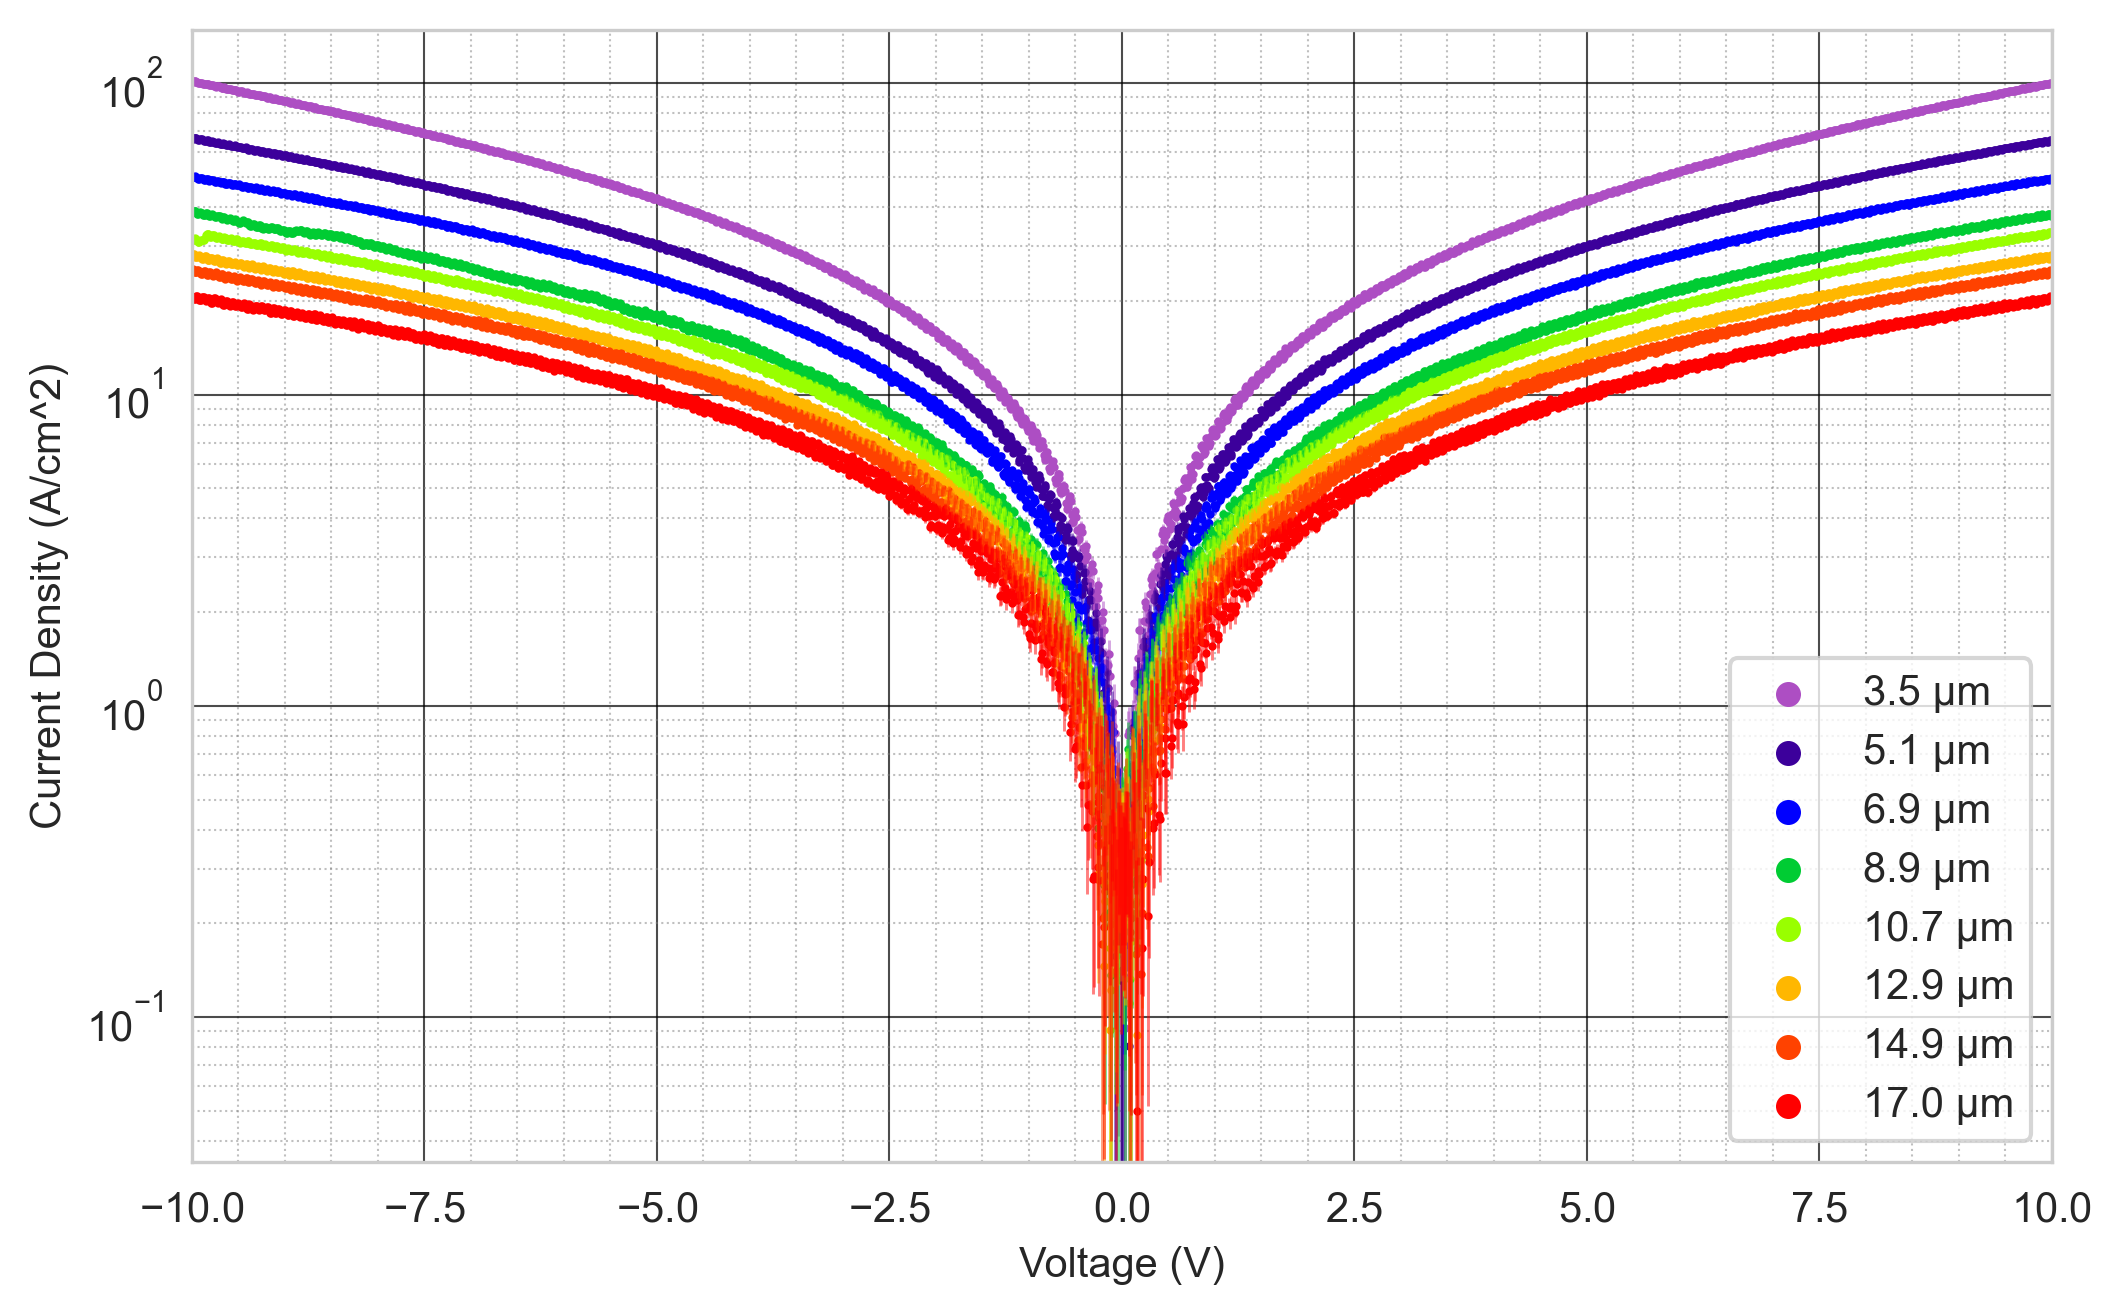
\includegraphics[width=0.97\textwidth]{Chapter3/Figs/Raster/Sample C 2019/10V_Current_Density_vs_Voltage_Temperature_21_log.png}
    \caption{A log-linear plot of the measured current density against applied voltage for all channel lengths at 21\si{\degreeCelsius} (sample C).}
    \label{appfig:current_density_21}
\end{figure}

\begin{figure}[h]
    \centering
    \includegraphics[width=0.97\textwidth]{Sample C 2019/10V_Current_Density_vs_Voltage_Temperature_50_log.png}
    \caption{A log-linear plot of the measured current density against applied voltage for all channel lengths at 50\si{\degreeCelsius} (sample C).}
    \label{appfig:current_density_50}
\end{figure}
\begin{figure}[h]
    \centering
    \includegraphics[width=0.97\textwidth]{Sample C 2019/10V_Current_Density_vs_Voltage_Temperature_100_log.png}
    \caption{A log-linear plot of the measured current density against applied voltage for all channel lengths at 100\si{\degreeCelsius} (sample C).}
    \label{appfig:current_density_100}
\end{figure}
\begin{figure}[h]
    \centering
    \includegraphics[width=0.97\textwidth]{Sample C 2019/10V_Current_Density_vs_Voltage_Temperature_150_log.png}
    \caption{A log-linear plot of the measured current density against applied voltage for all channel lengths at 150\si{\degreeCelsius} (sample C).}
    \label{appfig:current_density_150}
\end{figure}
\begin{figure}[h]
    \centering
    \includegraphics[width=0.97\textwidth]{Sample C 2019/10V_Current_Density_vs_Voltage_Temperature_200_log.png}
    \caption{A log-linear plot of the measured current density against applied voltage for all channel lengths at 200\si{\degreeCelsius} (sample C).}
    \label{appfig:current_density_200}
\end{figure}
\begin{figure}[h]
    \centering
    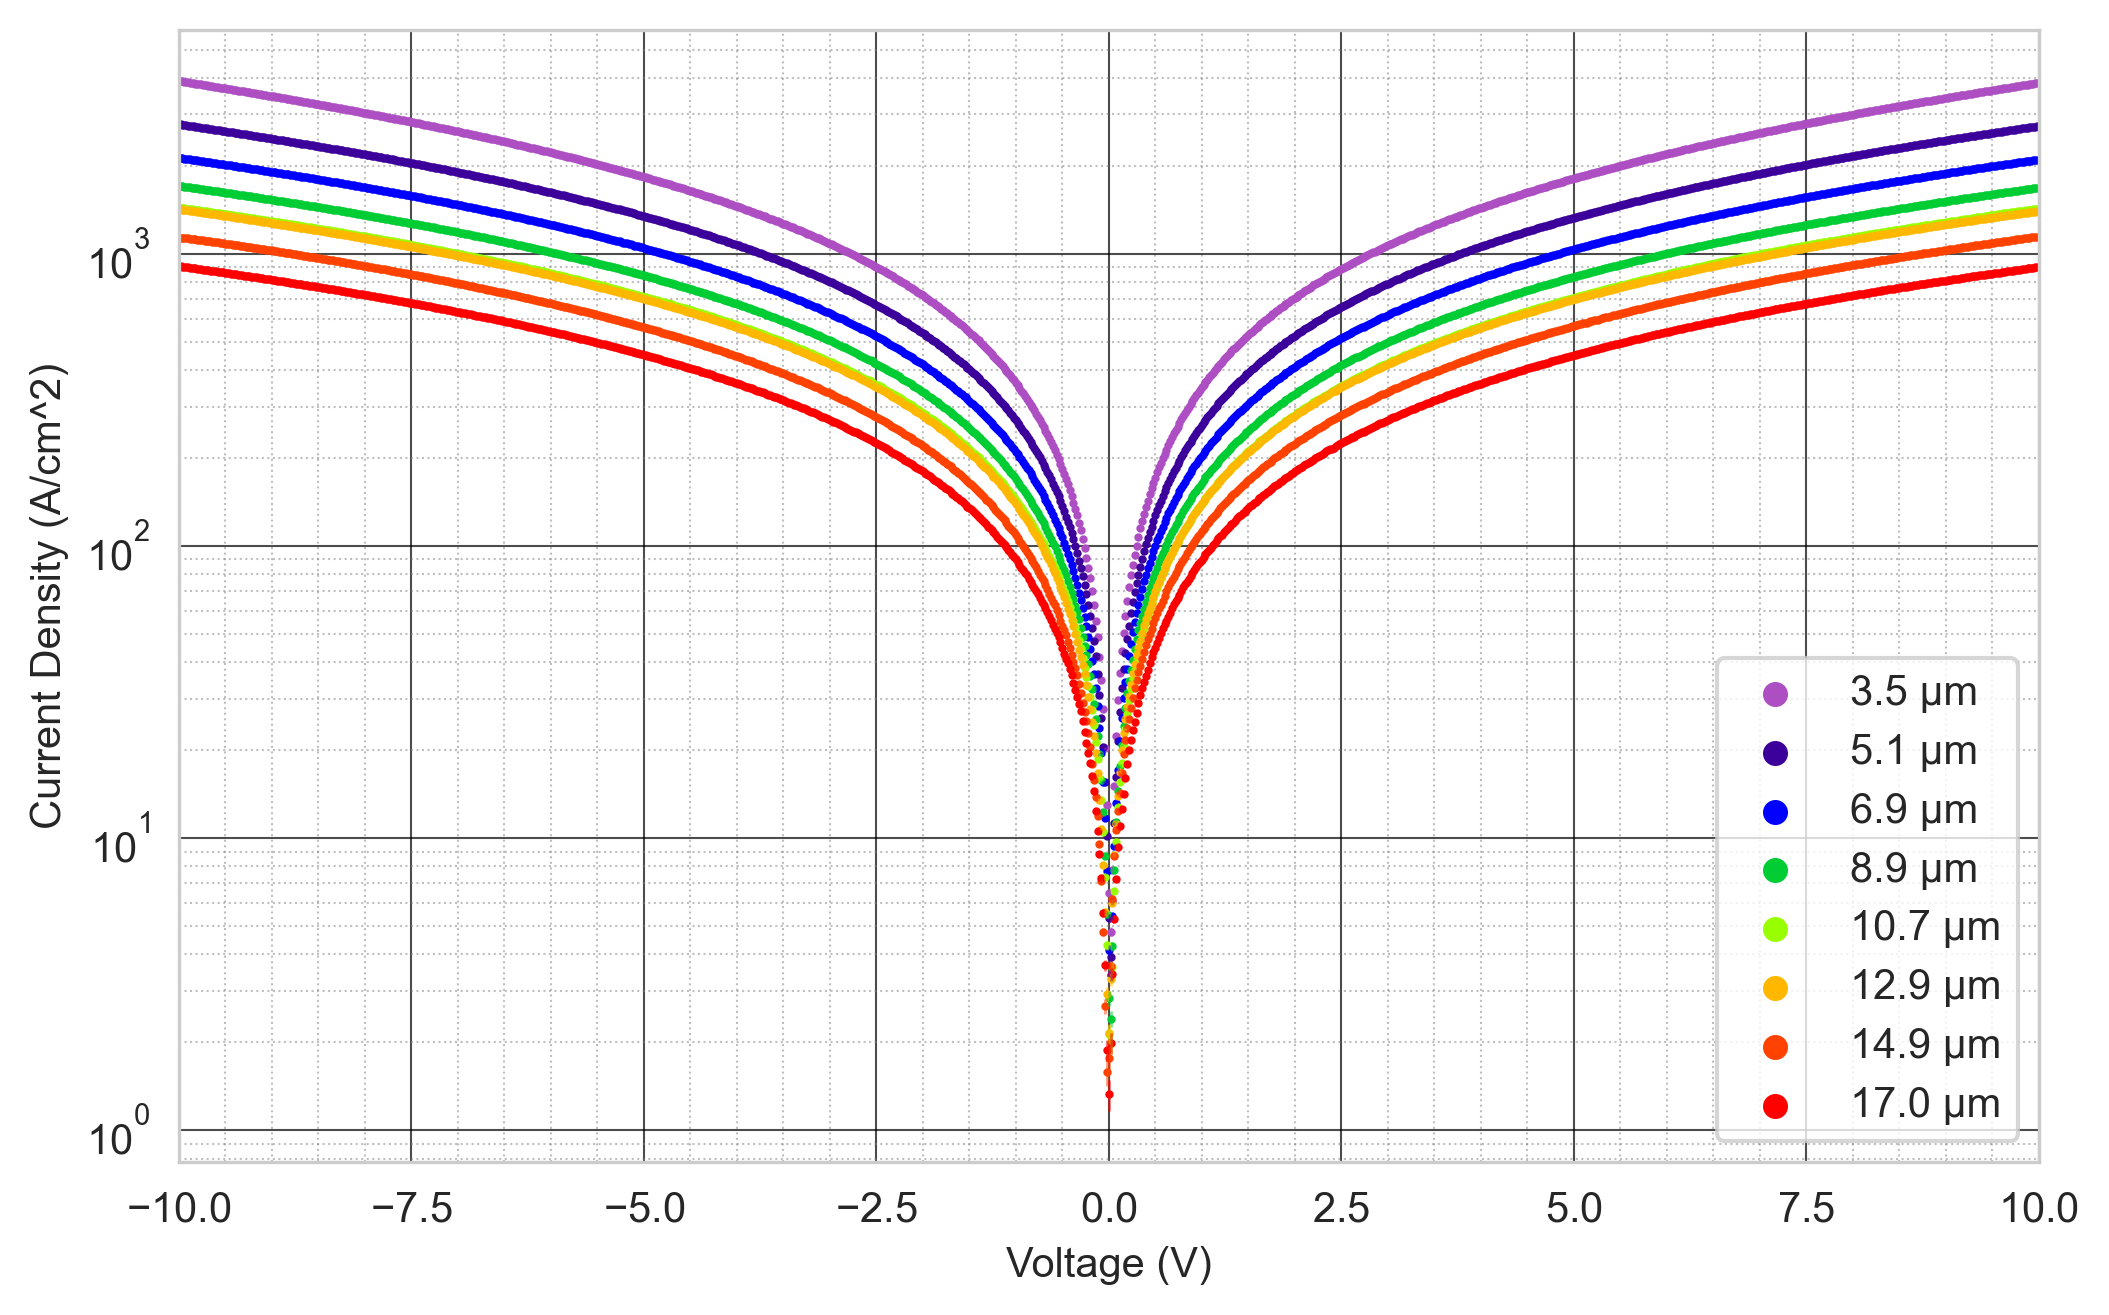
\includegraphics[width=0.97\textwidth]{Chapter3/Figs/Raster/Sample C 2019/10V_Current_Density_vs_Voltage_Temperature_250_log.png}
    \caption{A log-linear plot of the measured current density against applied voltage for all channel lengths at 250\si{\degreeCelsius} (sample C).}
    \label{appfig:current_density_250}
\end{figure}
\begin{figure}[h]
    \centering
    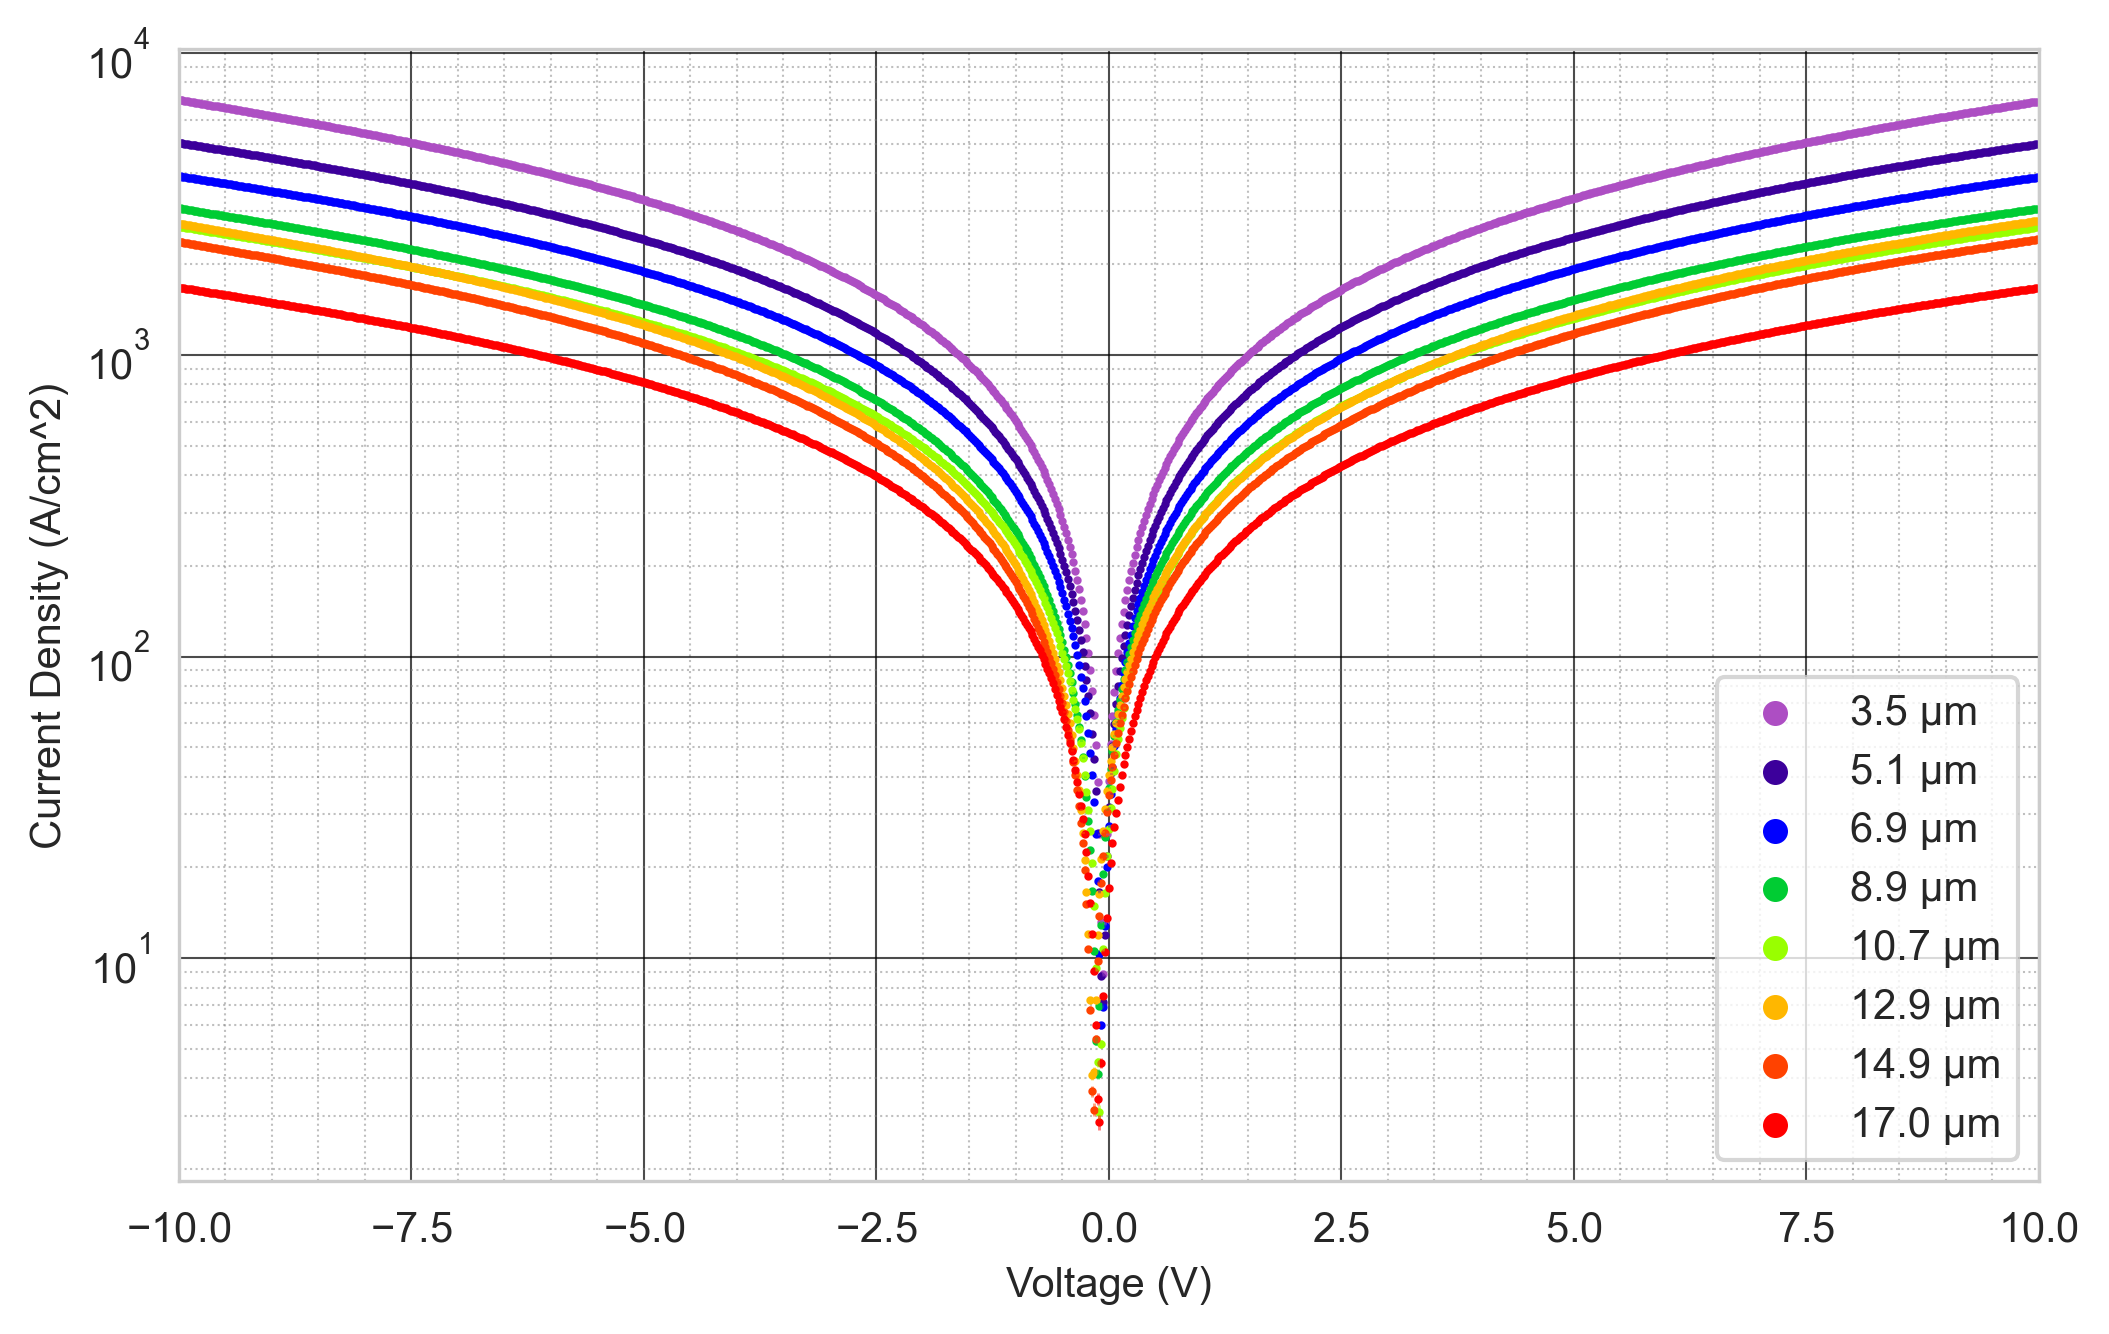
\includegraphics[width=0.97\textwidth]{Chapter3/Figs/Raster/Sample C 2019/10V_Current_Density_vs_Voltage_Temperature_300_log.png}
    \caption{A log-linear plot of the measured current density against applied voltage for all channel lengths at 300\si{\degreeCelsius} (sample C).}
    \label{appfig:current_density_300}
\end{figure}

\subsection{Sample D: 10 \si{\volt} range}
\label{app:J_V_sample_D_10V}

\begin{figure}[h]
    \centering
    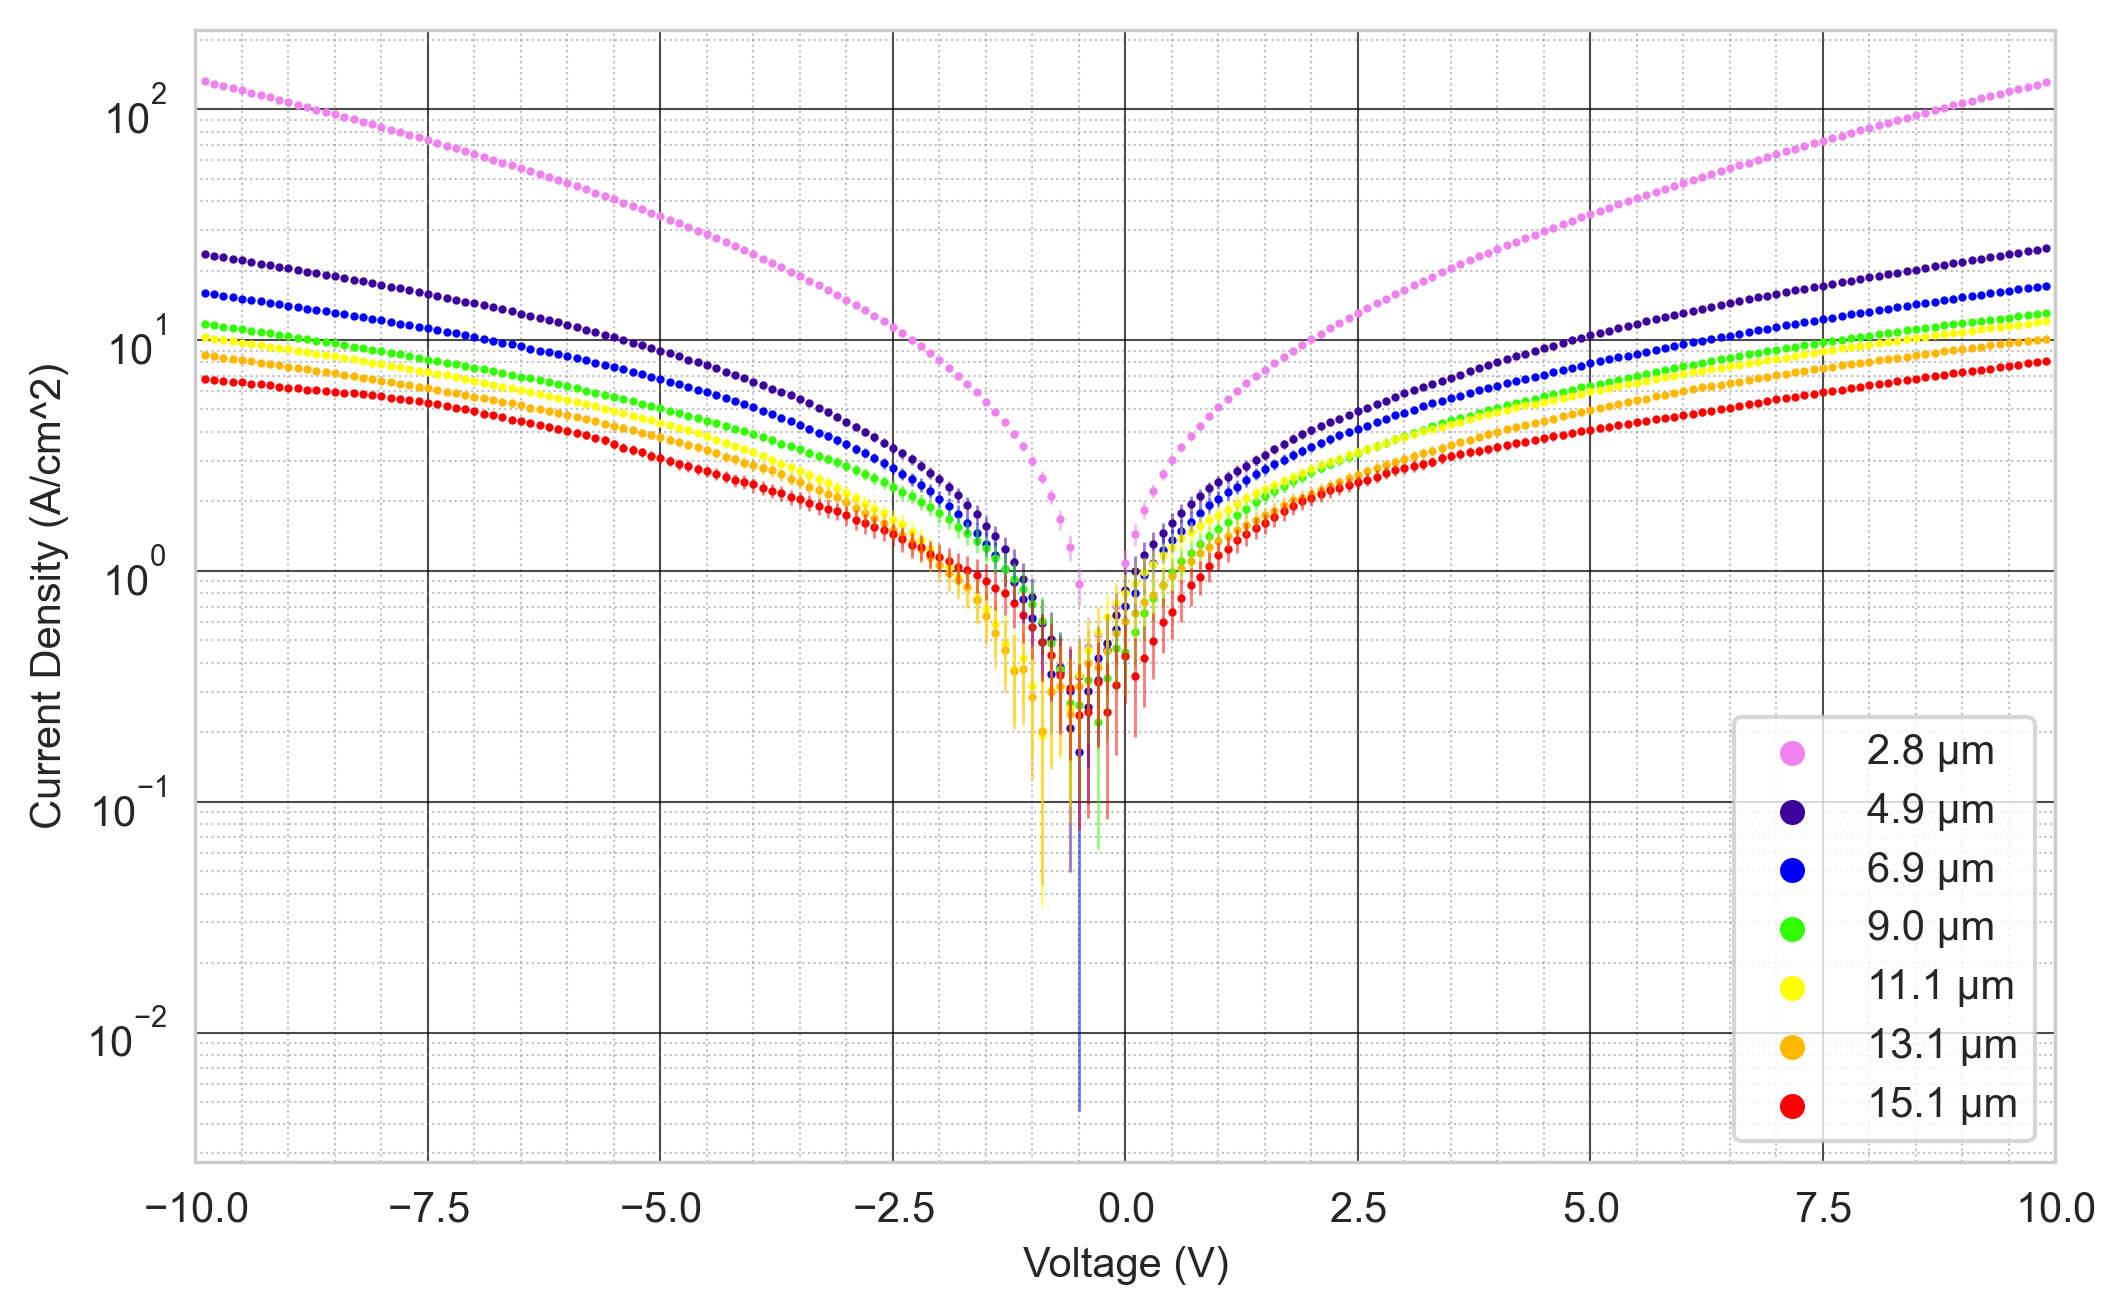
\includegraphics[width=0.97\textwidth]{Chapter3/Figs/Raster/Sample D 2019/10V_Current_Density_vs_Voltage_Temperature_21_log.png}
    \caption{A log-linear plot of the measured current density against applied voltage for all channel lengths at 21\si{\degreeCelsius} (sample D).}
    \label{appfig:10V_D_current_density_21}
\end{figure}
\begin{figure}[h]
    \centering
    \includegraphics[width=0.97\textwidth]{Sample D 2019/10V_Current_Density_vs_Voltage_Temperature_50_log.png}
    \caption{A log-linear plot of the measured current density against applied voltage for all channel lengths at 50\si{\degreeCelsius} (sample D).}
    \label{appfig:10V_D_current_density_50}
\end{figure}
\begin{figure}[h]
    \centering
    \includegraphics[width=0.97\textwidth]{Sample D 2019/10V_Current_Density_vs_Voltage_Temperature_100_log.png}
    \caption{A log-linear plot of the measured current density against applied voltage for all channel lengths at 100\si{\degreeCelsius} (sample D).}
    \label{appfig:10V_D_current_density_100}
\end{figure}
\begin{figure}[h]
    \centering
    \includegraphics[width=0.97\textwidth]{Sample D 2019/10V_Current_Density_vs_Voltage_Temperature_150_log.png}
    \caption{A log-linear plot of the measured current density against applied voltage for all channel lengths at 150\si{\degreeCelsius} (sample D).}
    \label{appfig:10V_D_current_density_150}
\end{figure}
\begin{figure}[h]
    \centering
    \includegraphics[width=0.97\textwidth]{Sample D 2019/10V_Current_Density_vs_Voltage_Temperature_200_log.png}
    \caption{A log-linear plot of the measured current density against applied voltage for all channel lengths at 200\si{\degreeCelsius} (sample D).}
    \label{appfig:10V_D_current_density_200}
\end{figure}
\begin{figure}[h]
    \centering
    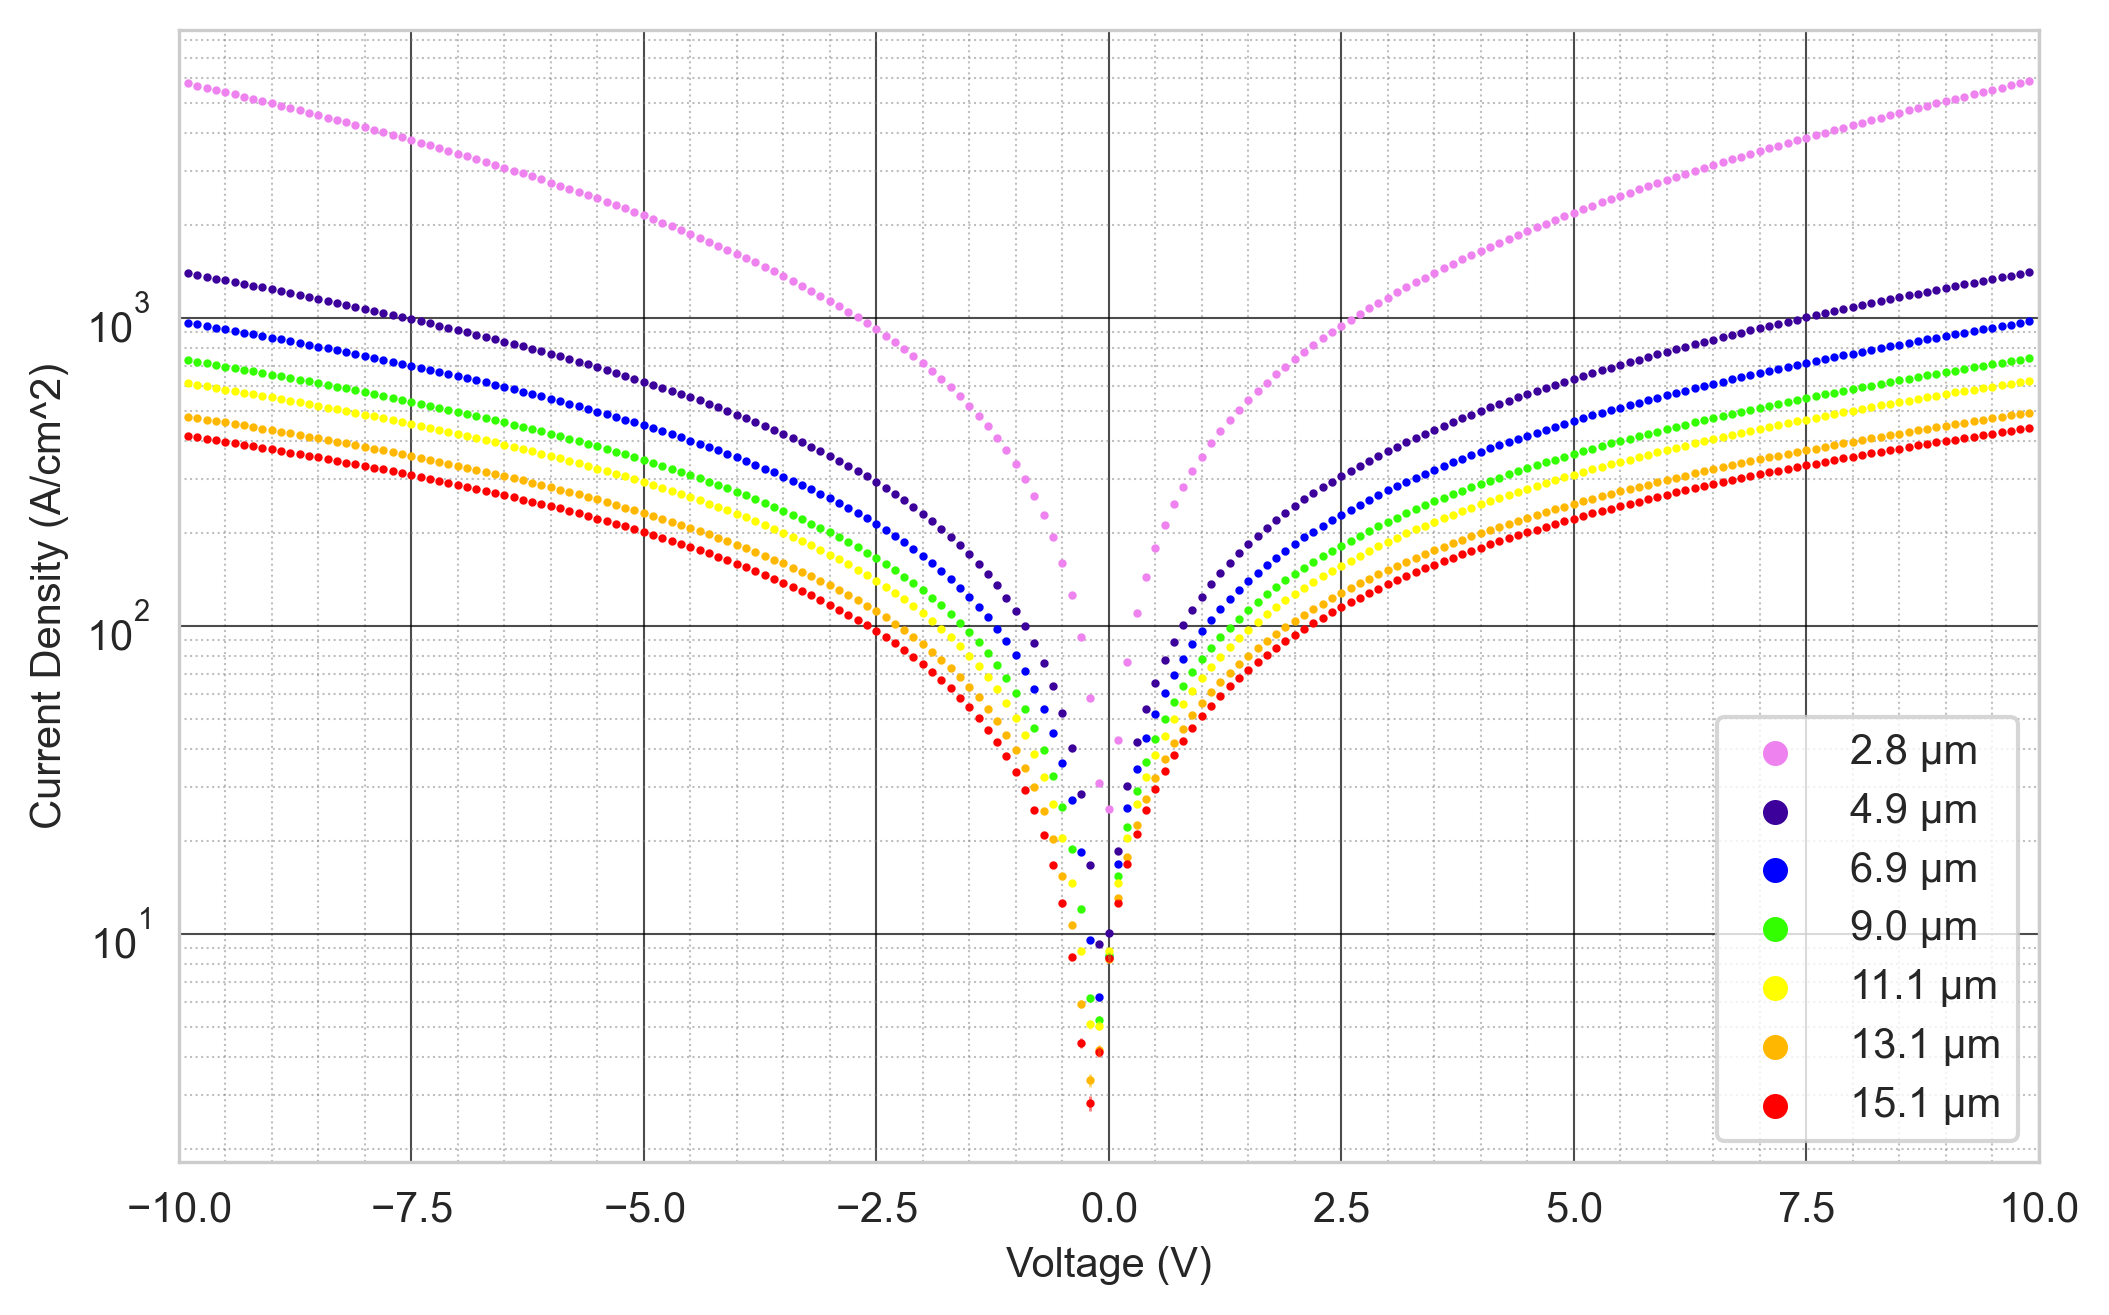
\includegraphics[width=0.97\textwidth]{Chapter3/Figs/Raster/Sample D 2019/10V_Current_Density_vs_Voltage_Temperature_250_log.png}
    \caption{A log-linear plot of the measured current density against applied voltage for all channel lengths at 250\si{\degreeCelsius} (sample D).}
    \label{appfig:10V_D_current_density_250}
\end{figure}
\begin{figure}[h]
    \centering
    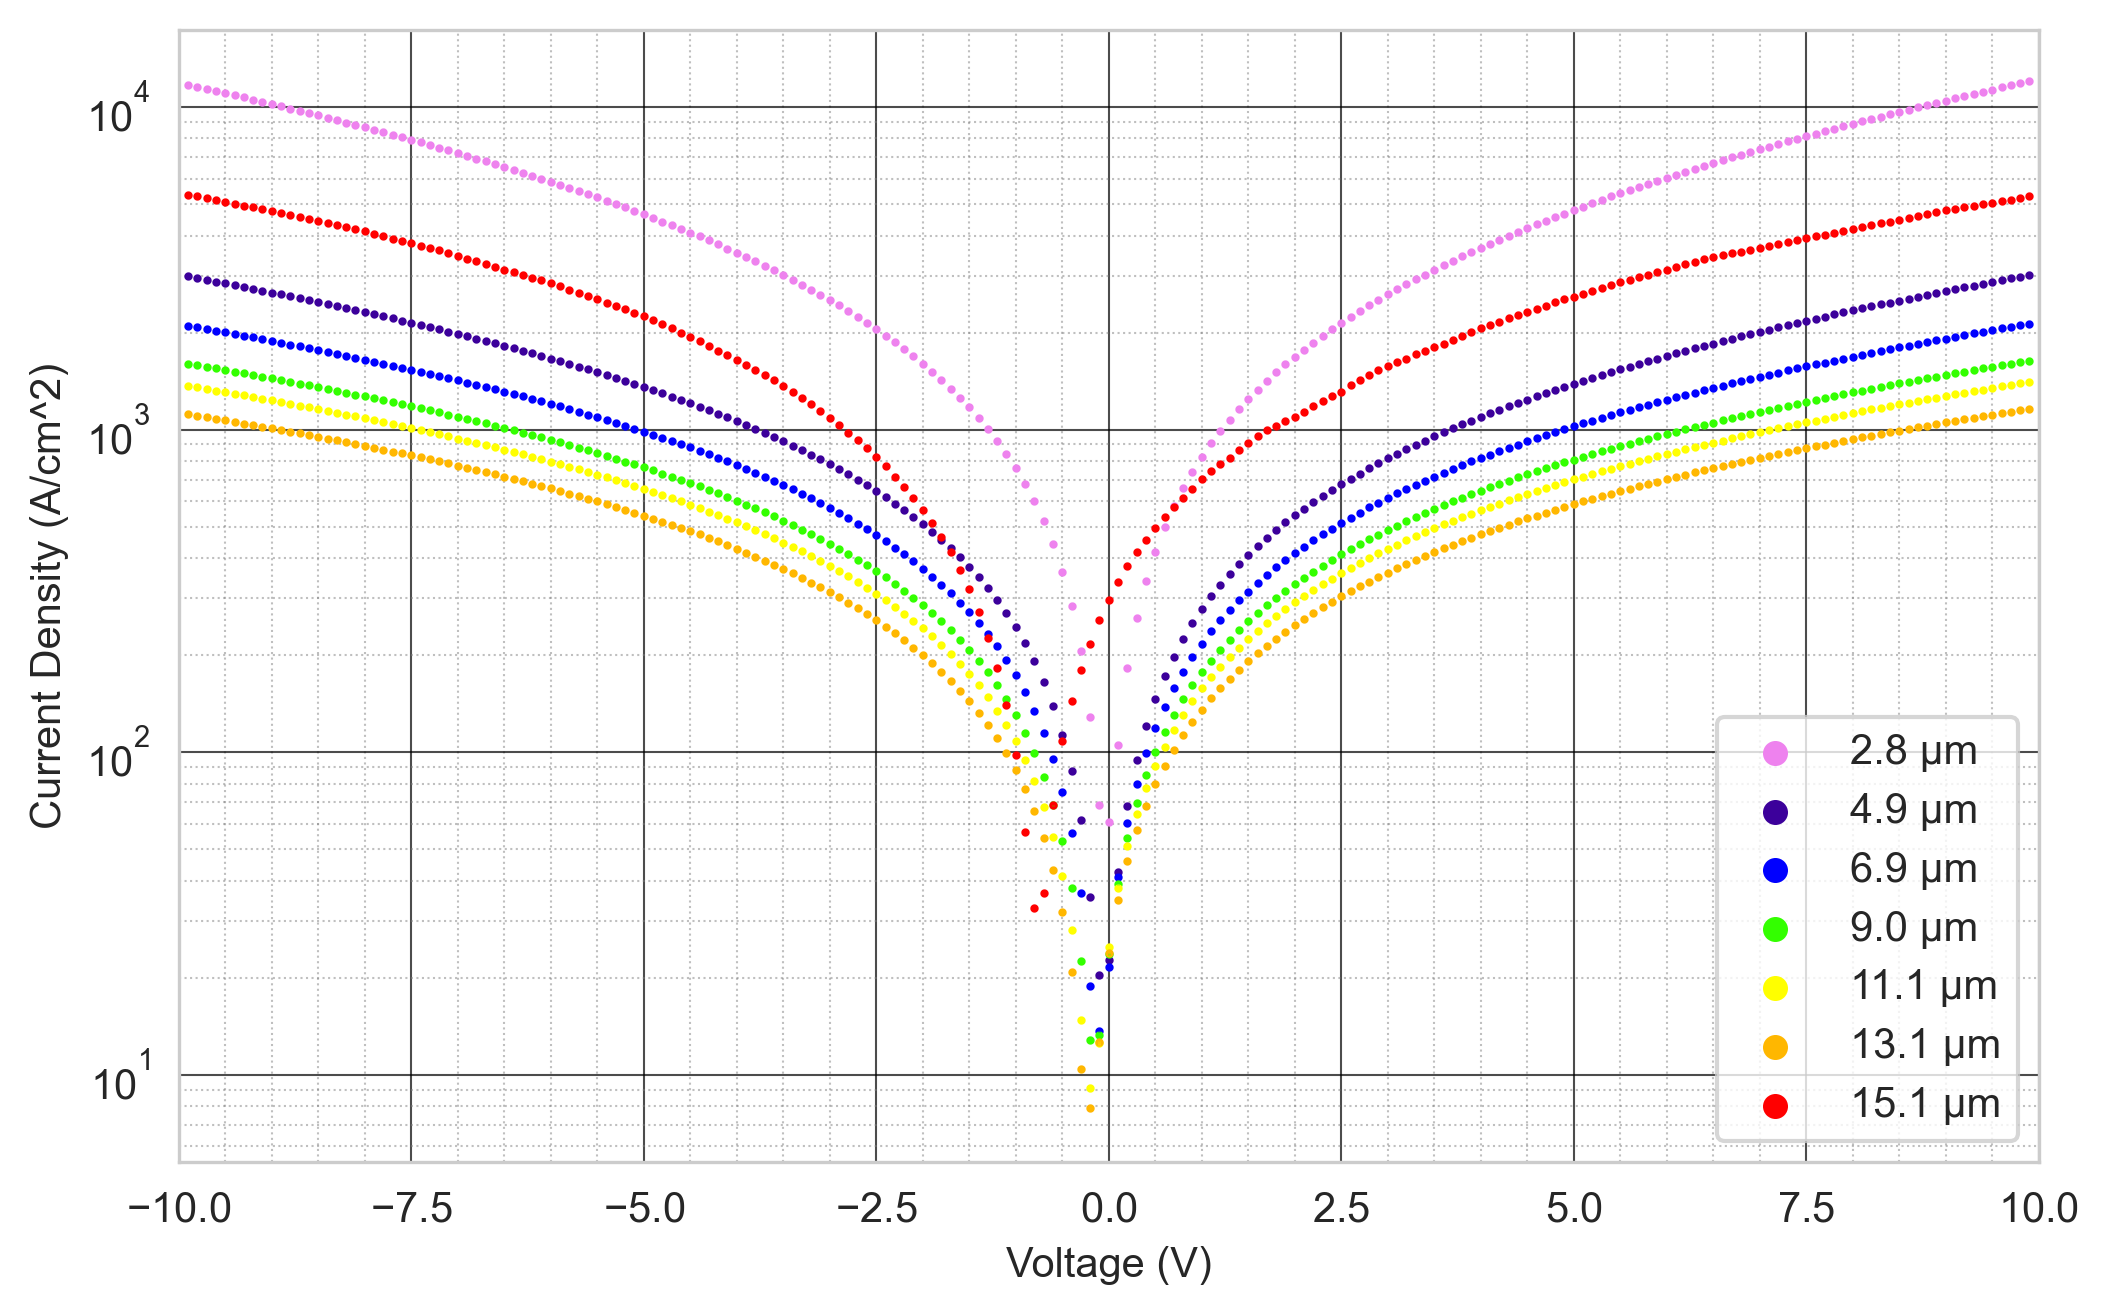
\includegraphics[width=0.97\textwidth]{Chapter3/Figs/Raster/Sample D 2019/10V_Current_Density_vs_Voltage_Temperature_300_log.png}
    \caption{A log-linear plot of the measured current density against applied voltage for all channel lengths at 300\si{\degreeCelsius} (sample D).}
    \label{appfig:10V_D_current_density_300}
\end{figure}

\subsection{Sample D: 50 \si{\volt} range}

\label{app:J_V_sample_D_50V}
\begin{figure}[h]
    \centering
    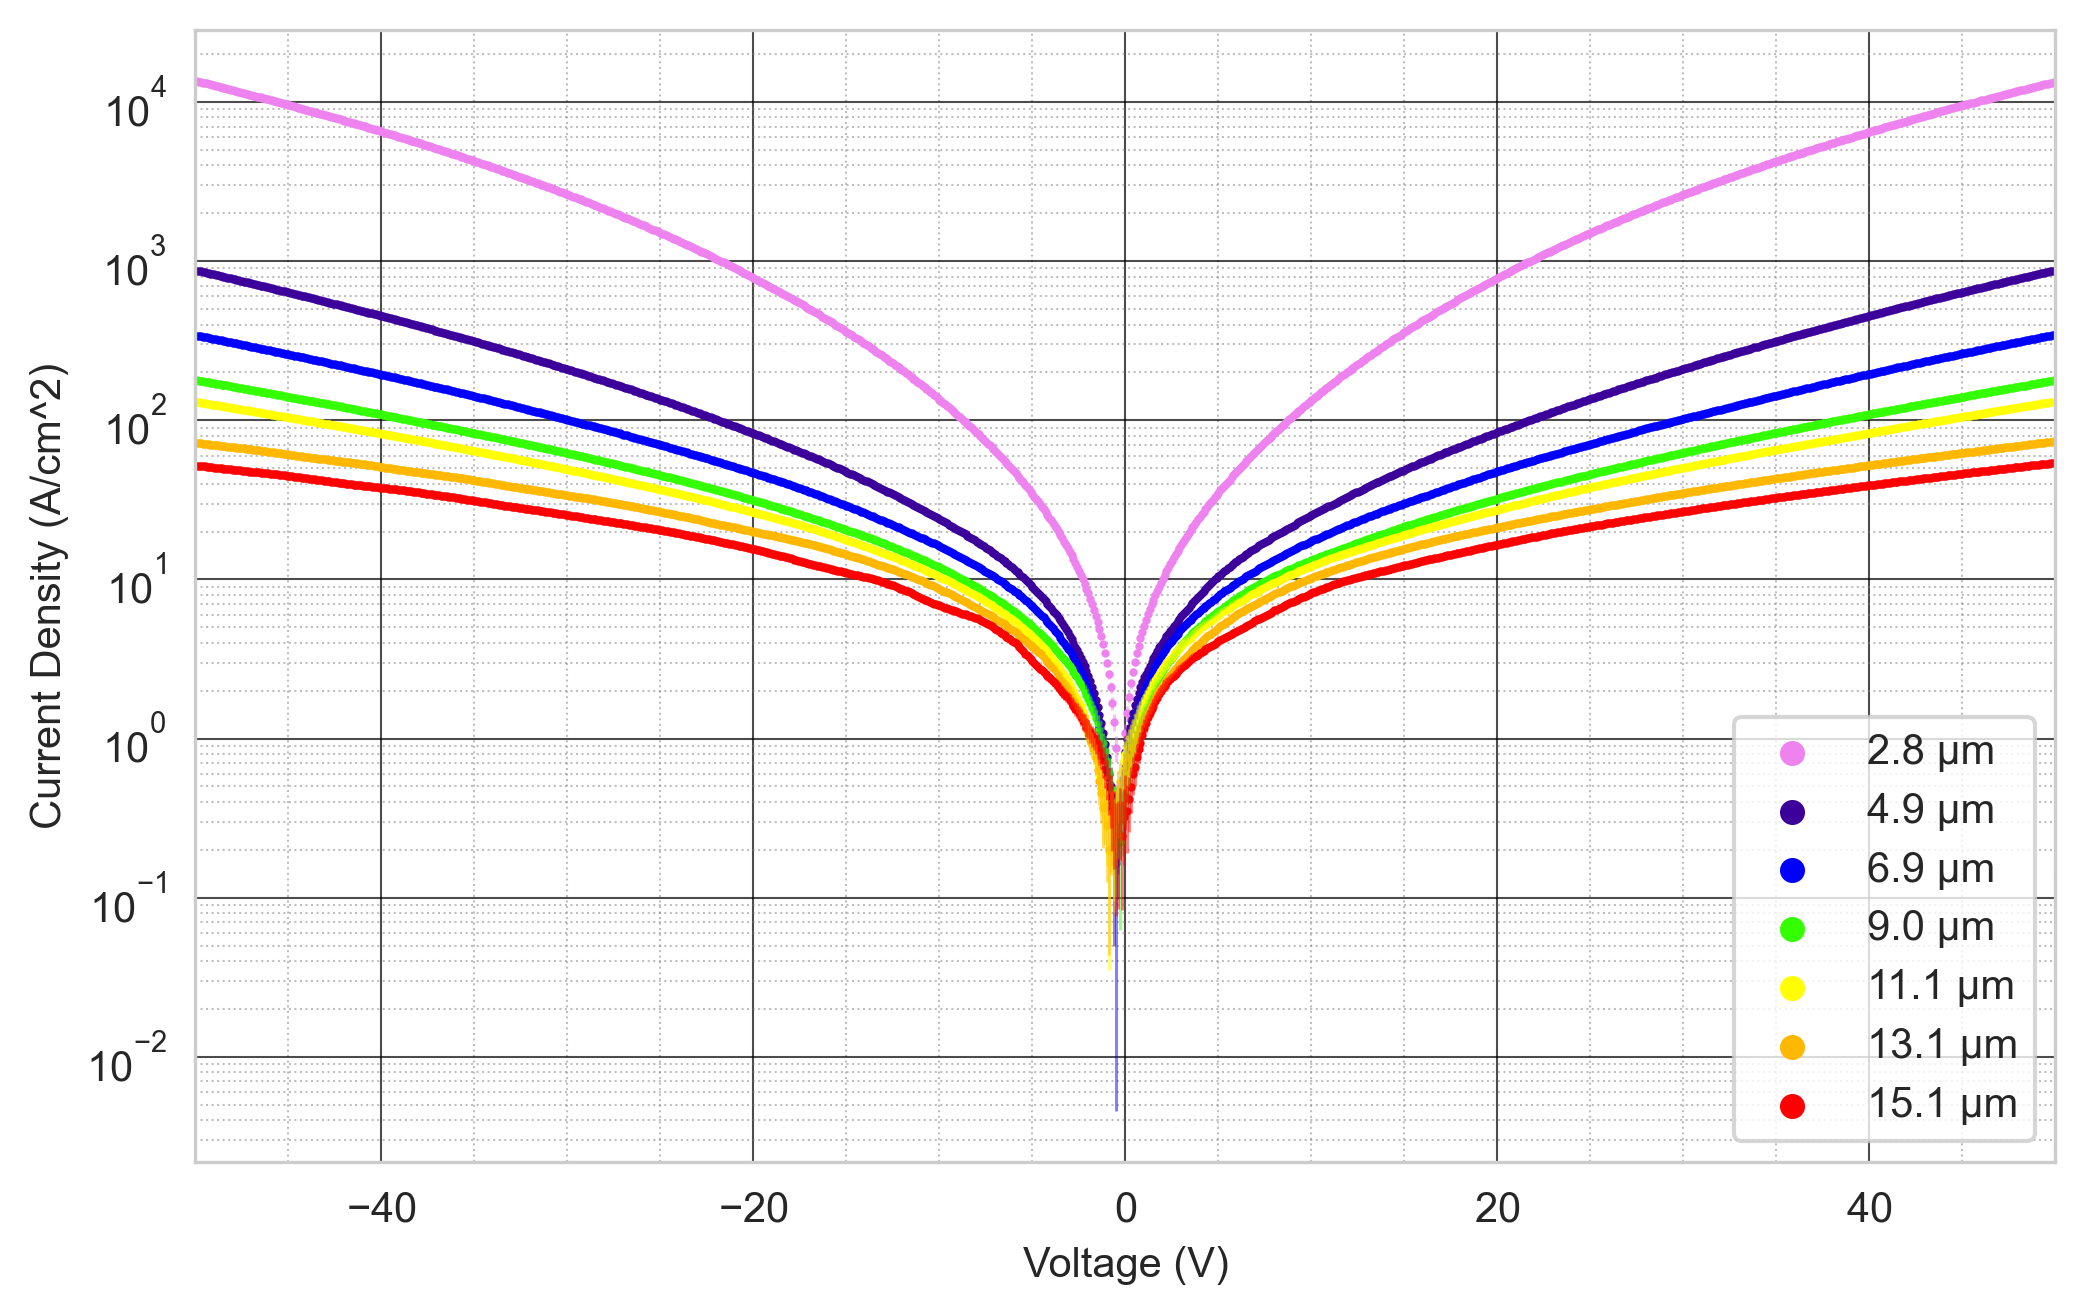
\includegraphics[width=0.97\textwidth]{Chapter3/Figs/Raster/Sample D 2019/50V_Current_Density_vs_Voltage_Temperature_21_log.png}
    \caption{A log-linear plot of the measured current density against applied voltage for all channel lengths at 21\si{\degreeCelsius} (sample D).}
    \label{appfig:D_current_density_21_50v}
\end{figure}
\begin{figure}[h]
    \centering
    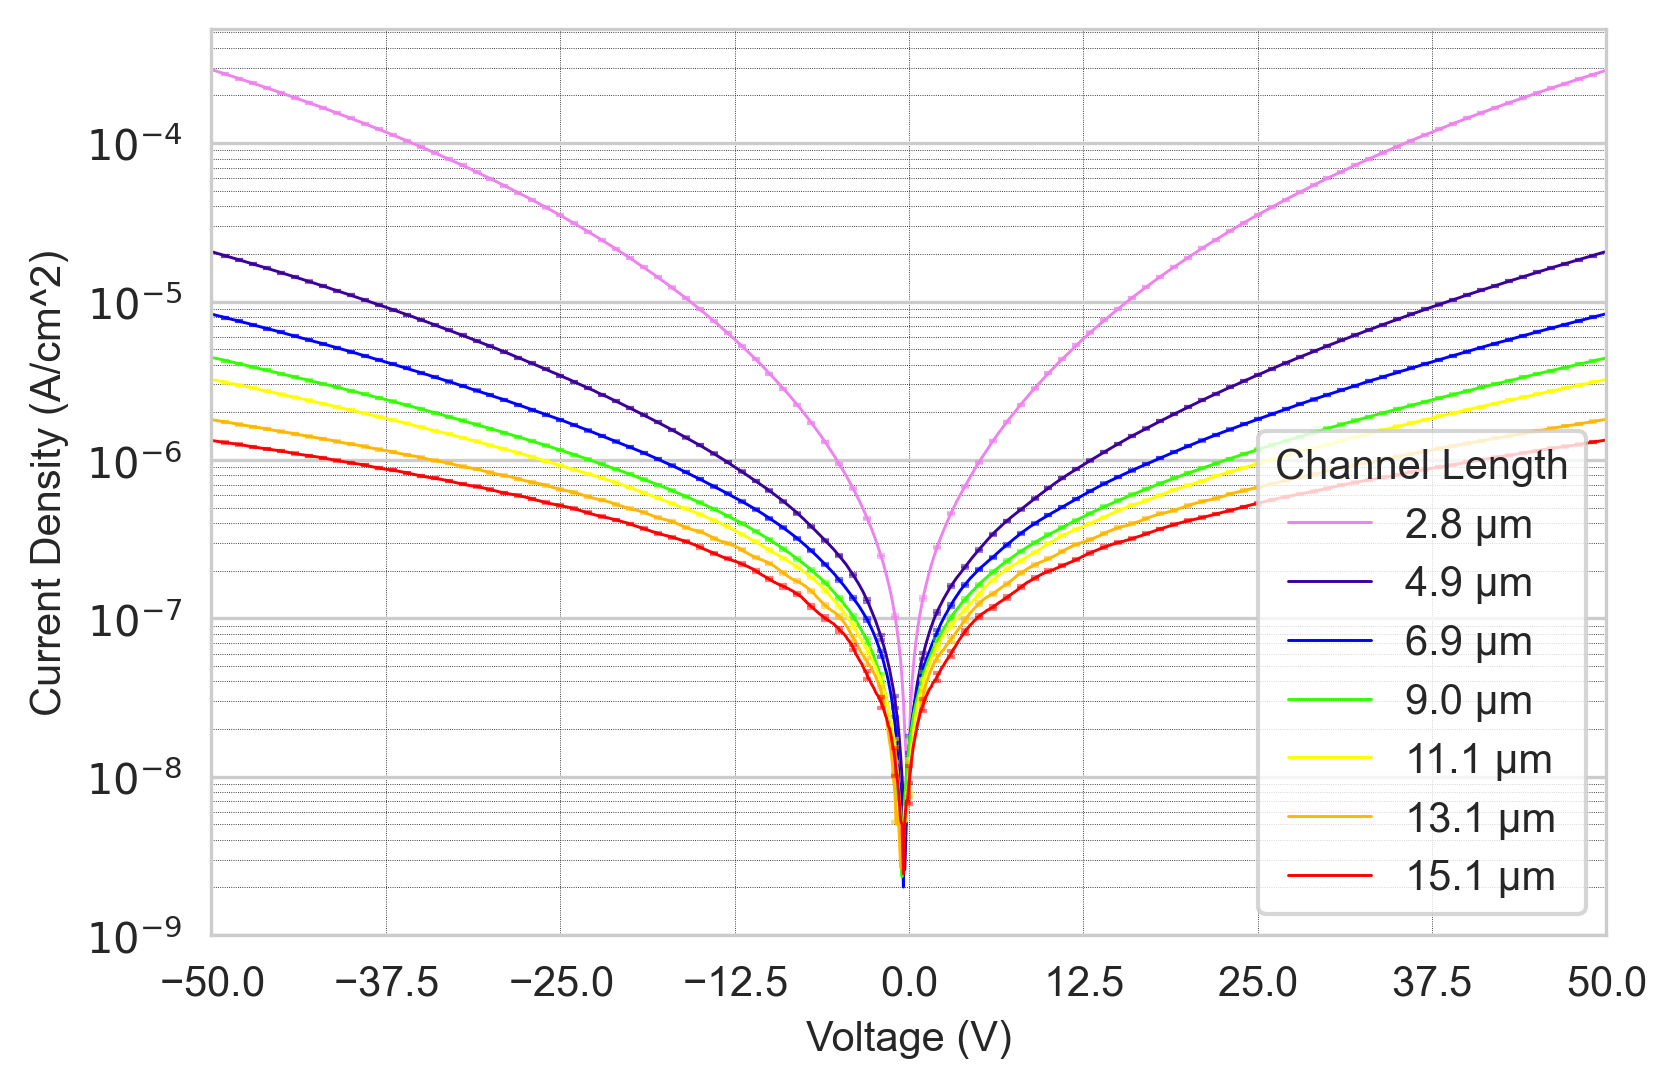
\includegraphics[width=0.97\textwidth]{Sample D 2019/50V_Current_Density_vs_Voltage_Temperature_50_log.png}
    \caption{A log-linear plot of the measured current density against applied voltage for all channel lengths at 50\si{\degreeCelsius} (sample D).}
    \label{appfig:D_current_density_50_50v}
\end{figure}
\begin{figure}[h]
    \centering
    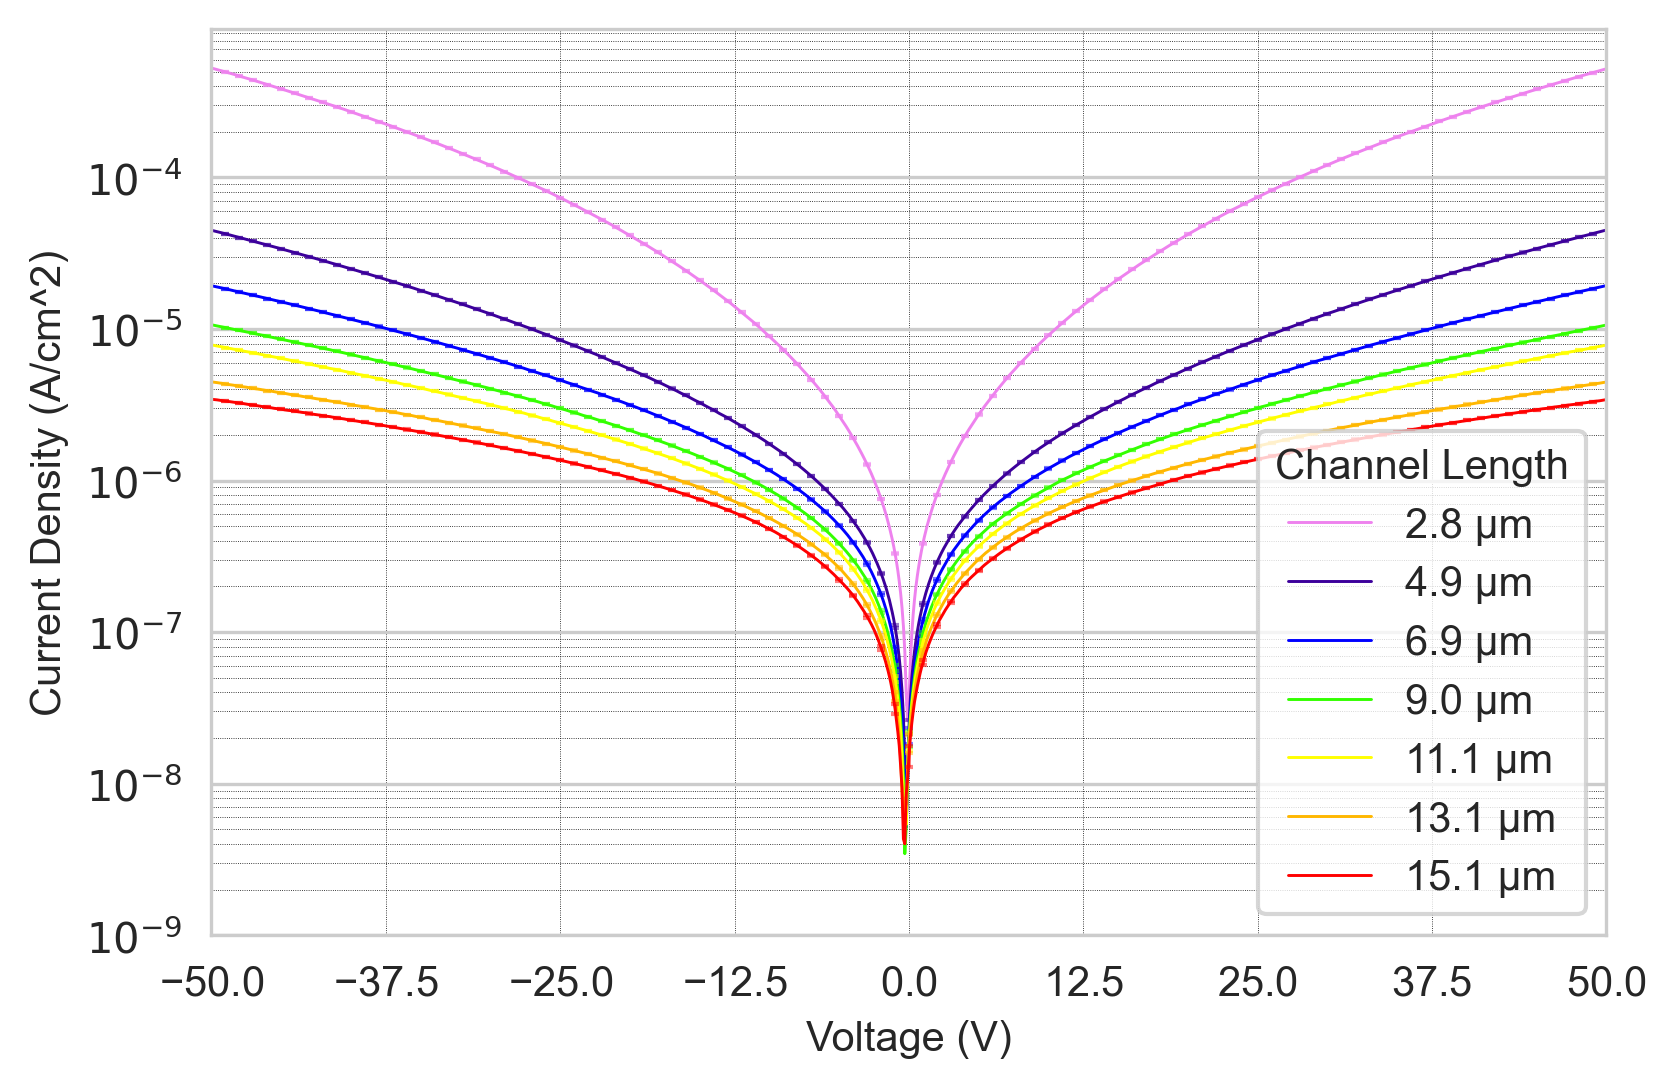
\includegraphics[width=0.97\textwidth]{Sample D 2019/50V_Current_Density_vs_Voltage_Temperature_100_log.png}
    \caption{A log-linear plot of the measured current density against applied voltage for all channel lengths at 100\si{\degreeCelsius} (sample D).}
    \label{appfig:D_current_density_100_50}
\end{figure}
\begin{figure}[h]
    \centering
    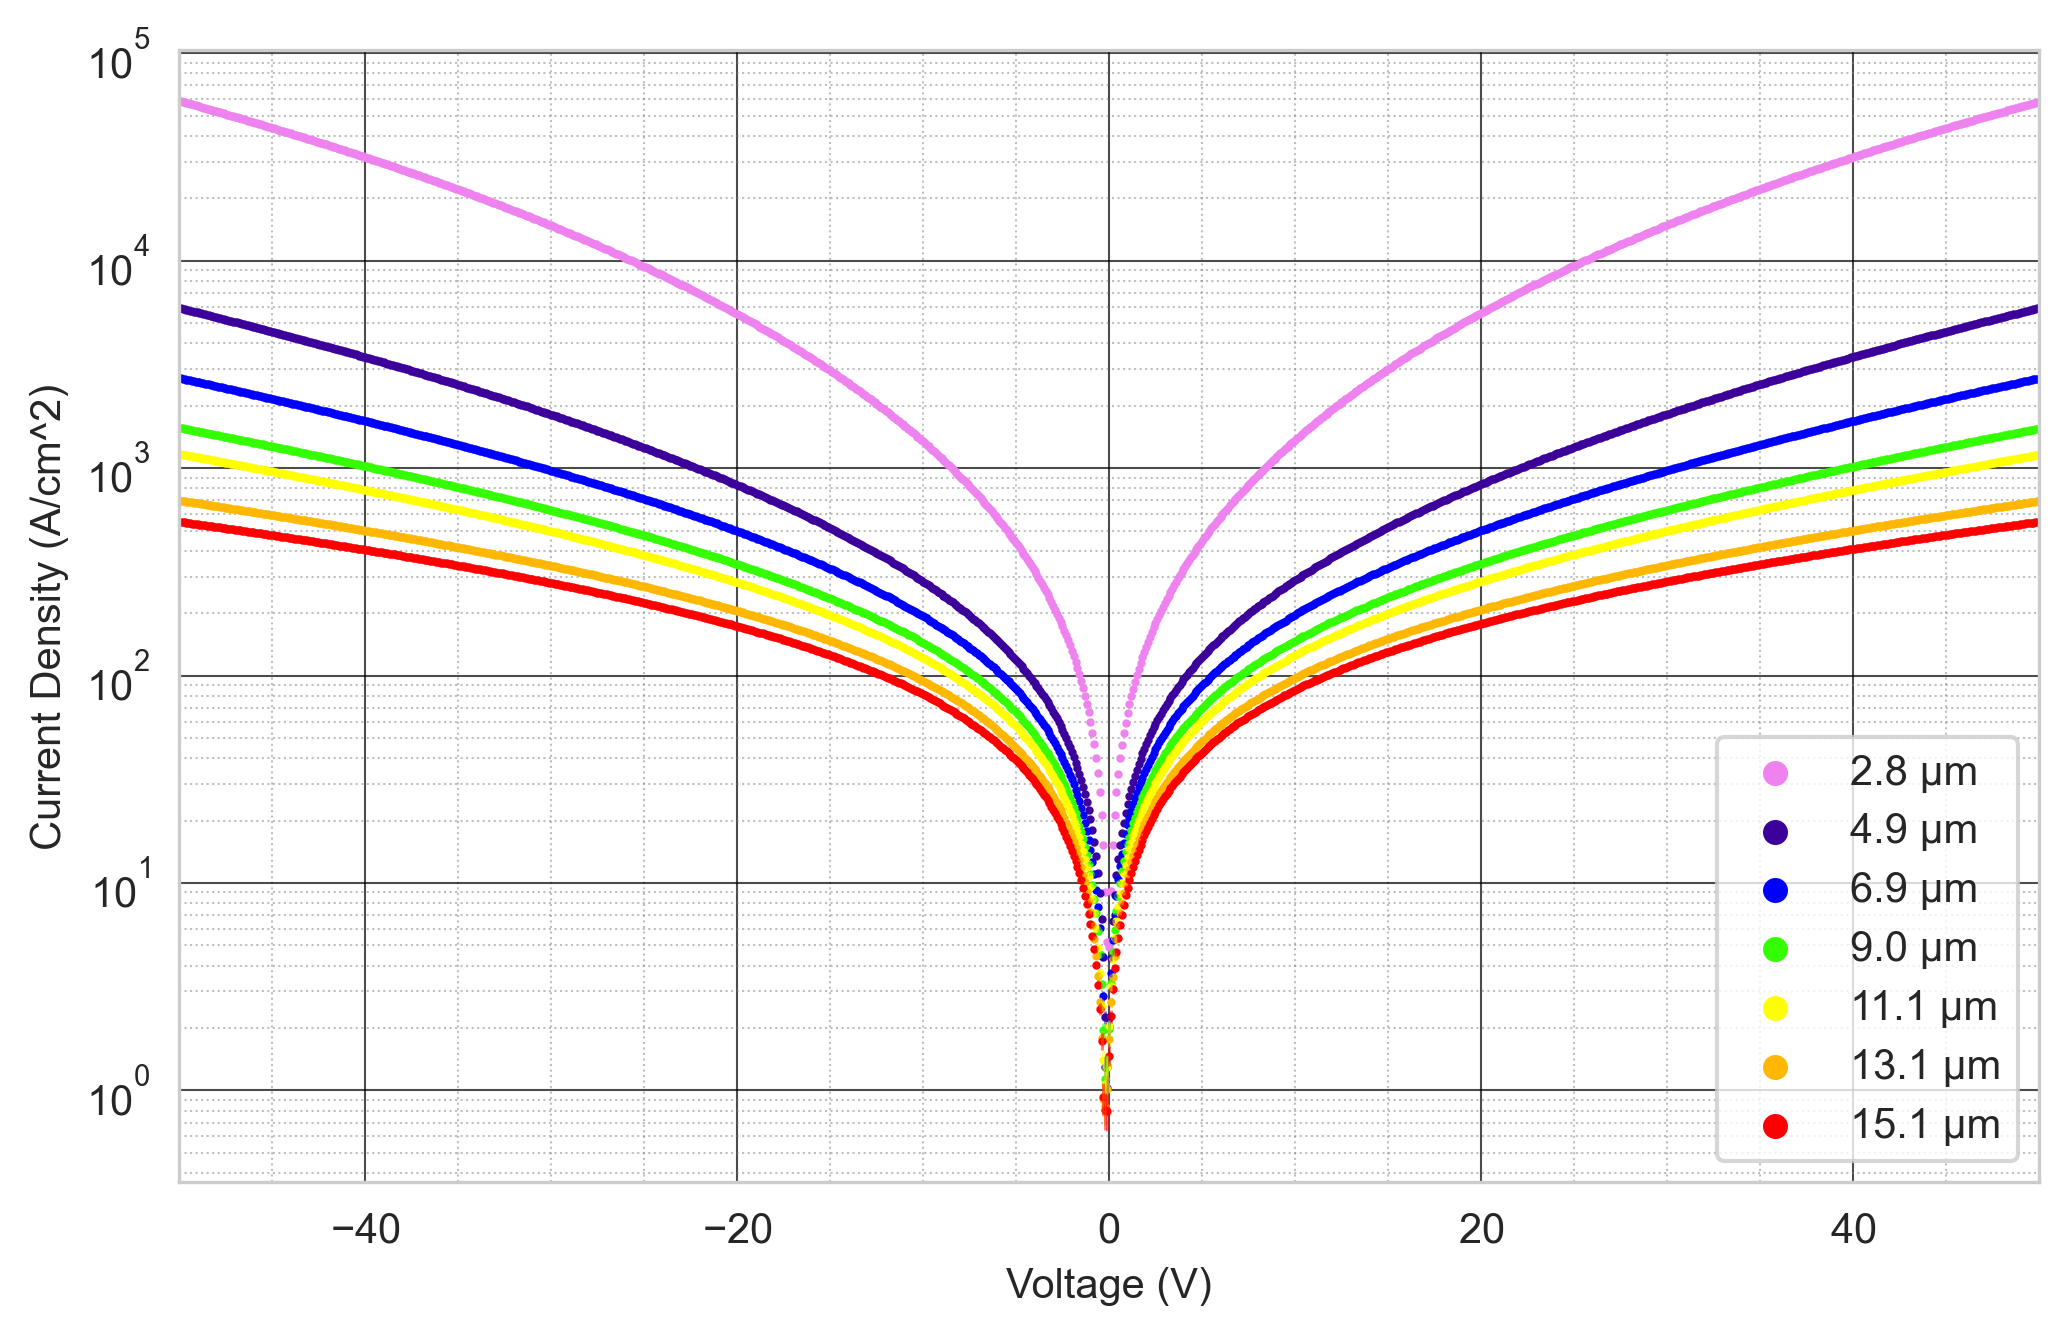
\includegraphics[width=0.97\textwidth]{Sample D 2019/50V_Current_Density_vs_Voltage_Temperature_150_log.png}
    \caption{A log-linear plot of the measured current density against applied voltage for all channel lengths at 150\si{\degreeCelsius} (sample D).}
    \label{appfig:D_current_density_150_50v}
\end{figure}
\begin{figure}[h]
    \centering
    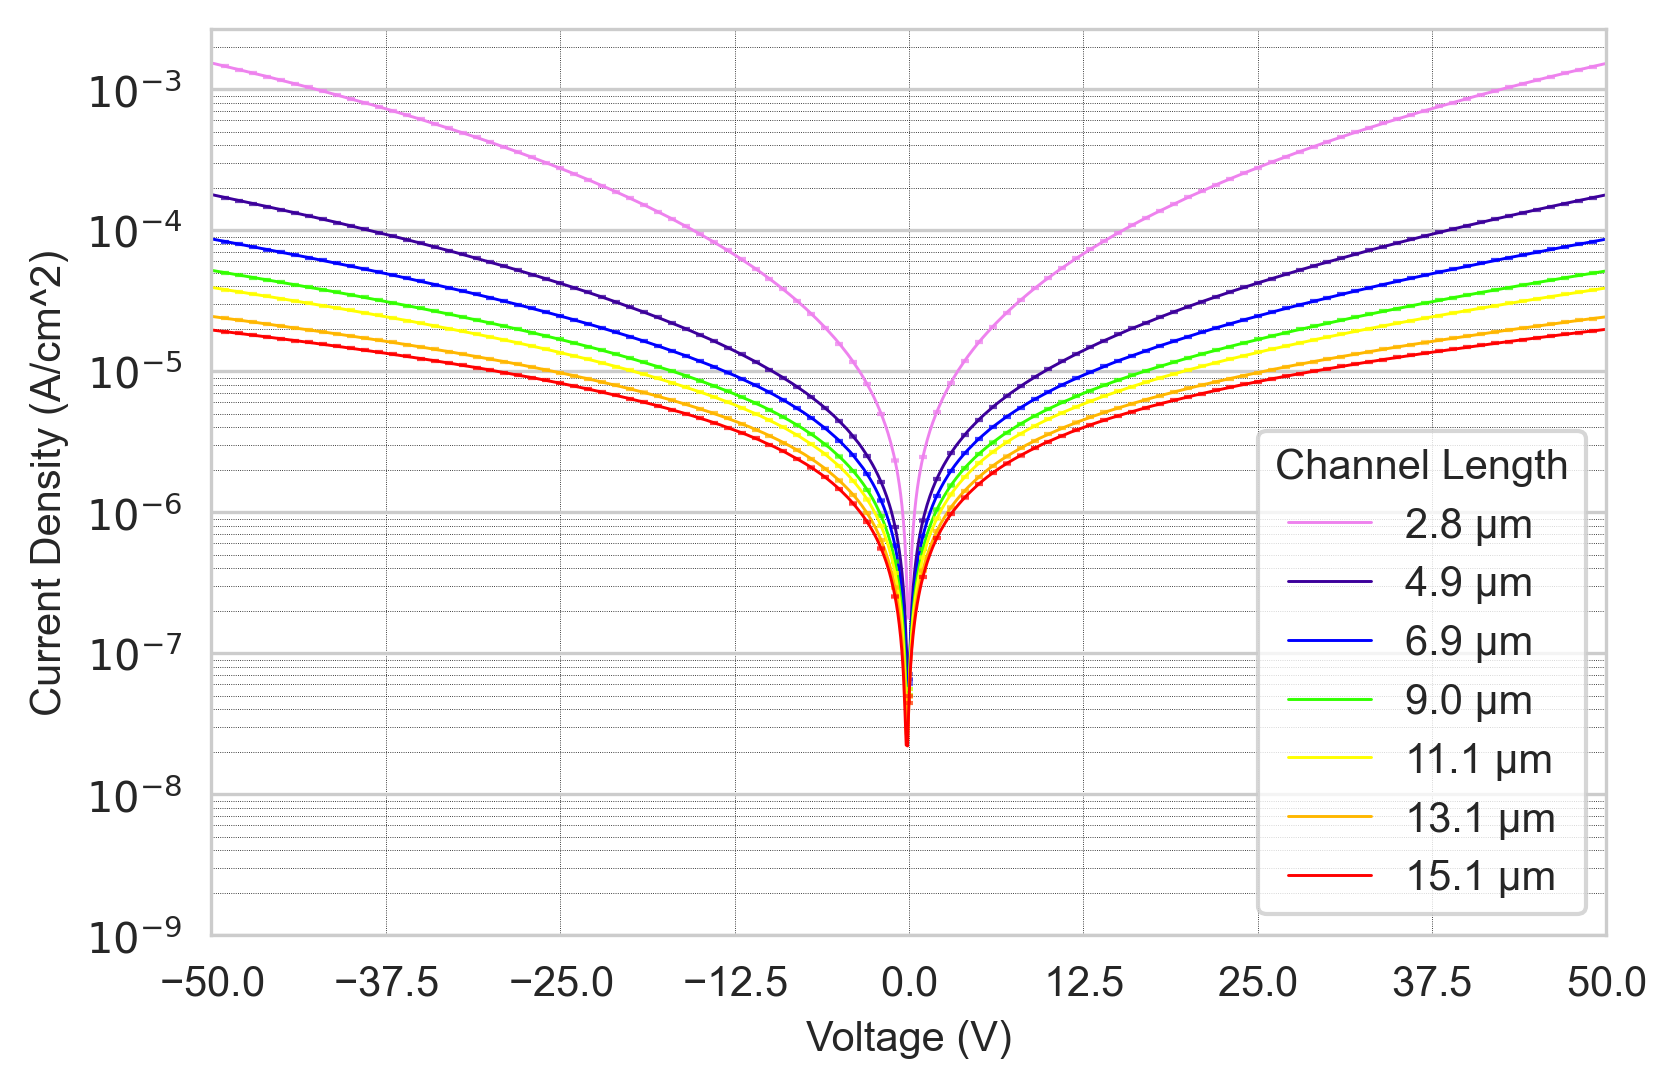
\includegraphics[width=0.97\textwidth]{Sample D 2019/50V_Current_Density_vs_Voltage_Temperature_200_log.png}
    \caption{A log-linear plot of the measured current density against applied voltage for all channel lengths at 200\si{\degreeCelsius} (sample D).}
    \label{appfig:D_current_density_200_50v}
\end{figure}
\begin{figure}[h]
    \centering
    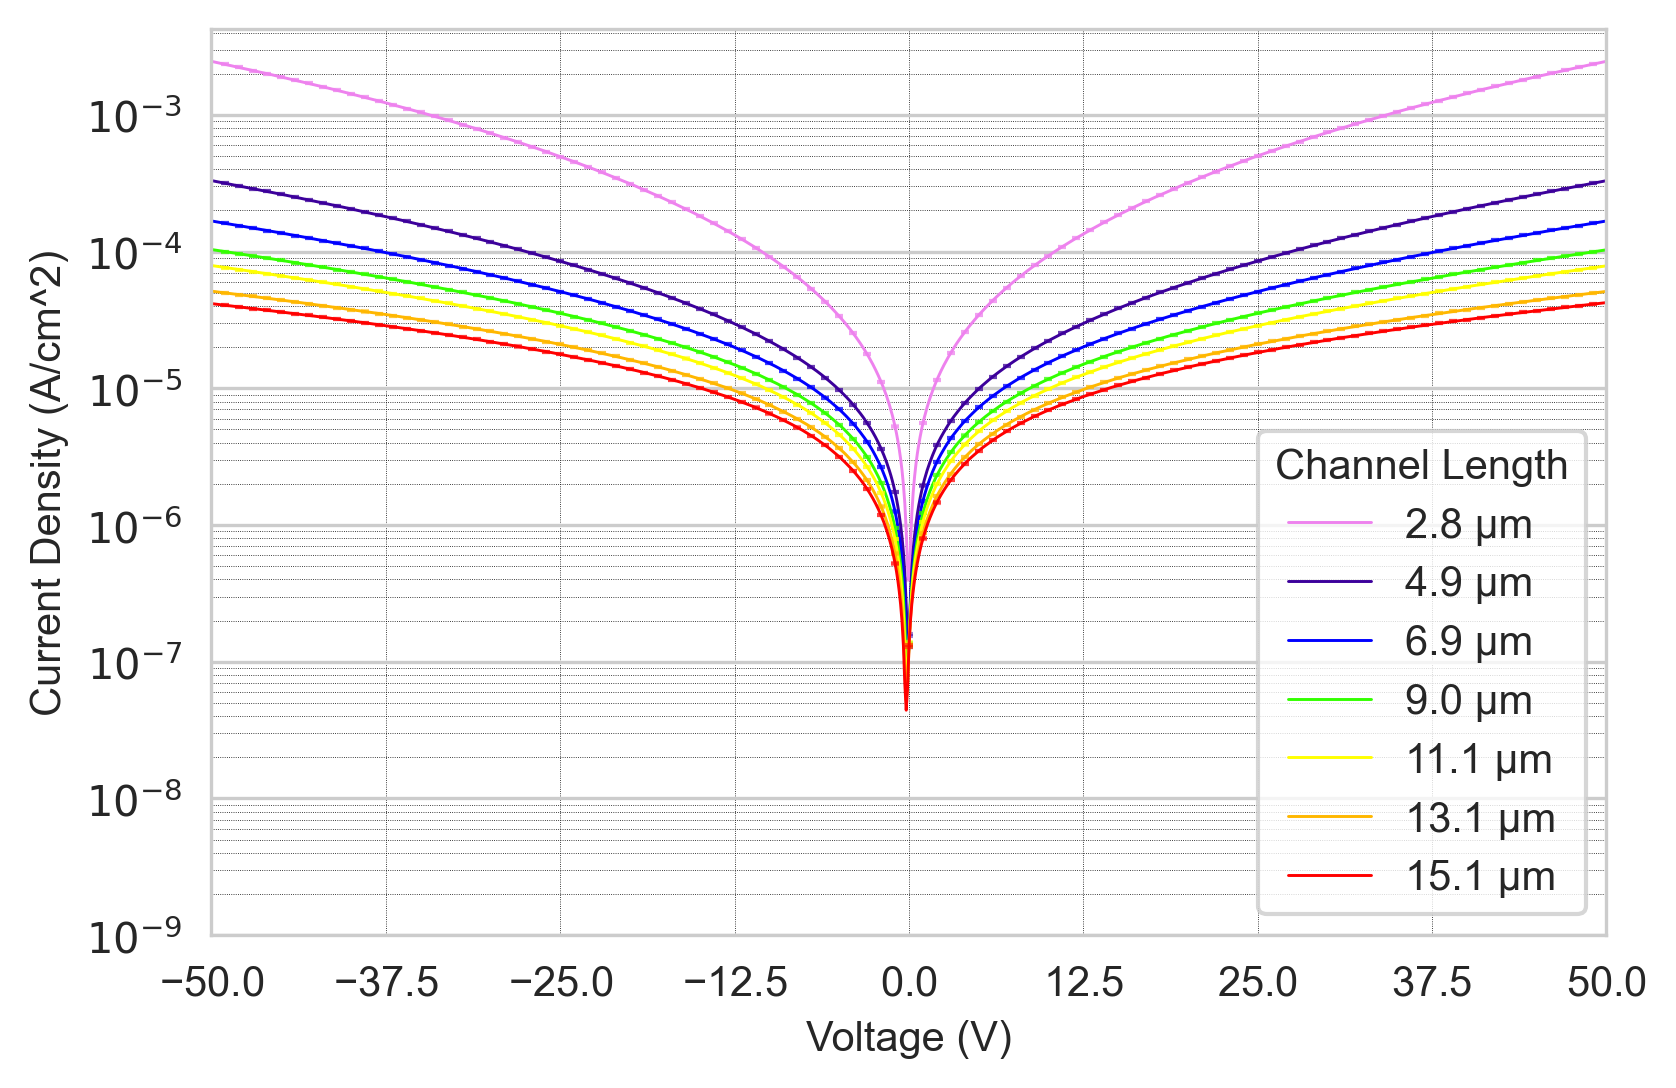
\includegraphics[width=0.97\textwidth]{Sample D 2019/50V_Current_Density_vs_Voltage_Temperature_250_log.png}
    \caption{A log-linear plot of the measured current density against applied voltage for all channel lengths at 250\si{\degreeCelsius} (sample D).}
    \label{appfig:D_current_density_250_50v}
\end{figure}
\begin{figure}[h]
    \centering
    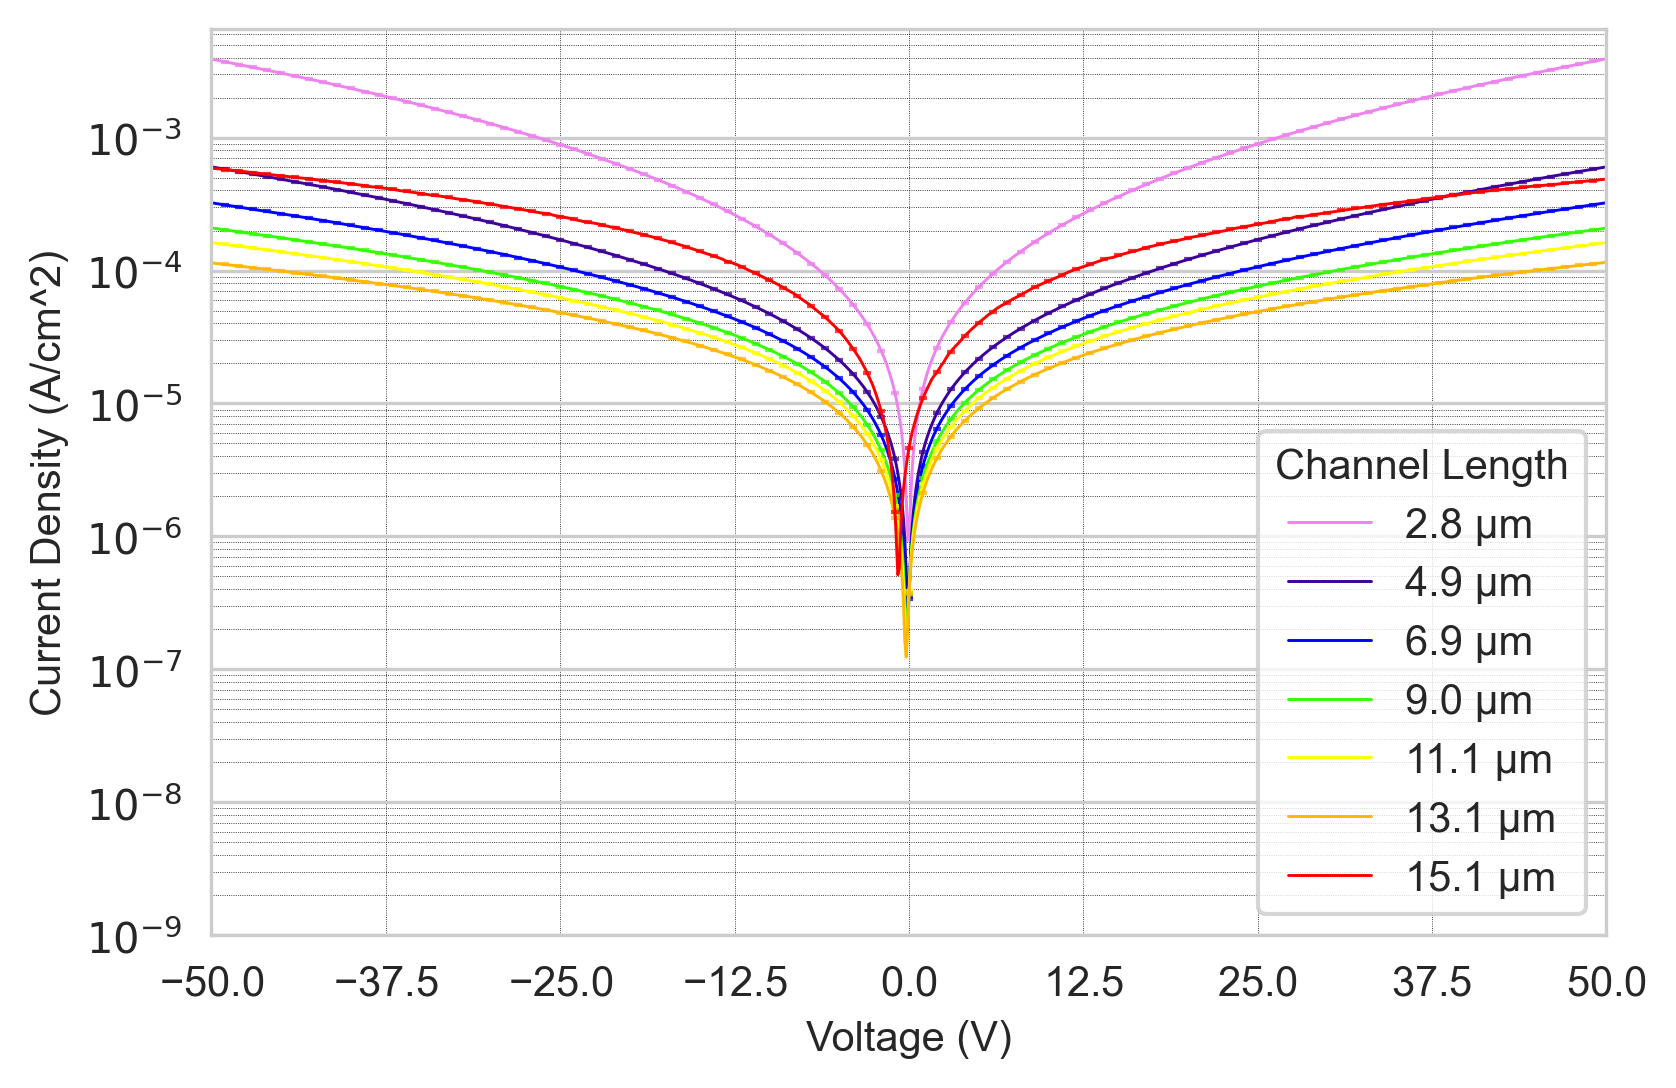
\includegraphics[width=0.97\textwidth]{Sample D 2019/50V_Current_Density_vs_Voltage_Temperature_300_log.png}
    \caption{A log-linear plot of the measured current density against applied voltage for all channel lengths at 300\si{\degreeCelsius} (sample D).}
    \label{appfig:D_current_density_300_50v}
\end{figure}

\section{LTLM I-V, samples C and D}
\label{app:LTLM_I_V_data}

For reference, error bars of 2 \si{\pico\ampere} are plotted on a limited bias range of $\pm1$ \si{\volt} in figure \ref{appfig:1V_C_current_voltage_21}.

\begin{figure}[h]
    \centering
    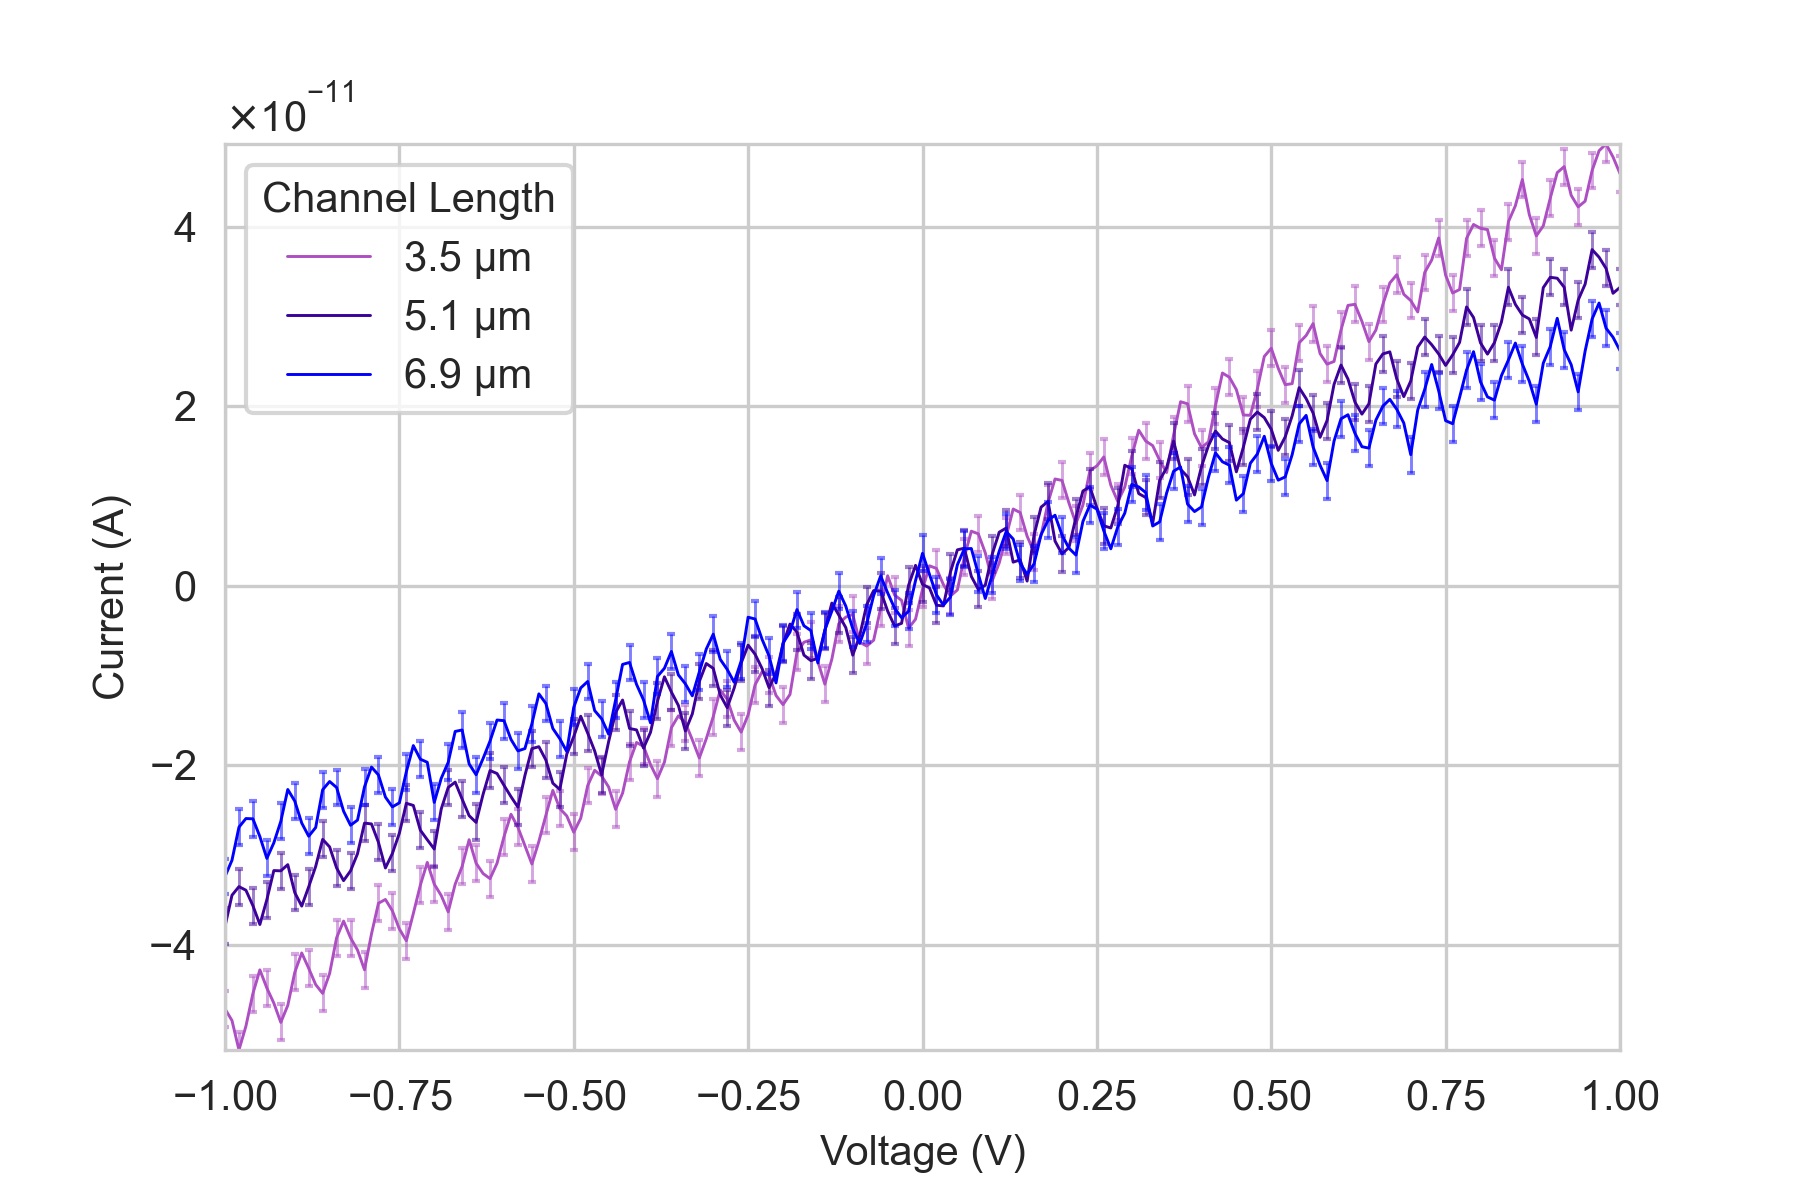
\includegraphics[width=0.97\textwidth]{Appendix1/1V IV characteristics at 21 C.png}
    \caption{A linear plot of the measured current against applied voltage for three channel lengths, $\pm1$ \si{\volt}, with 2 \si{\pico\ampere} error bars at 21\si{\degreeCelsius} (sample C).}
    \label{appfig:1V_C_current_voltage_21}
\end{figure}

\subsection{Sample C: 10 \si{\volt} range}
\label{app:I_V_sample_C}

\begin{figure}[h]
    \centering
    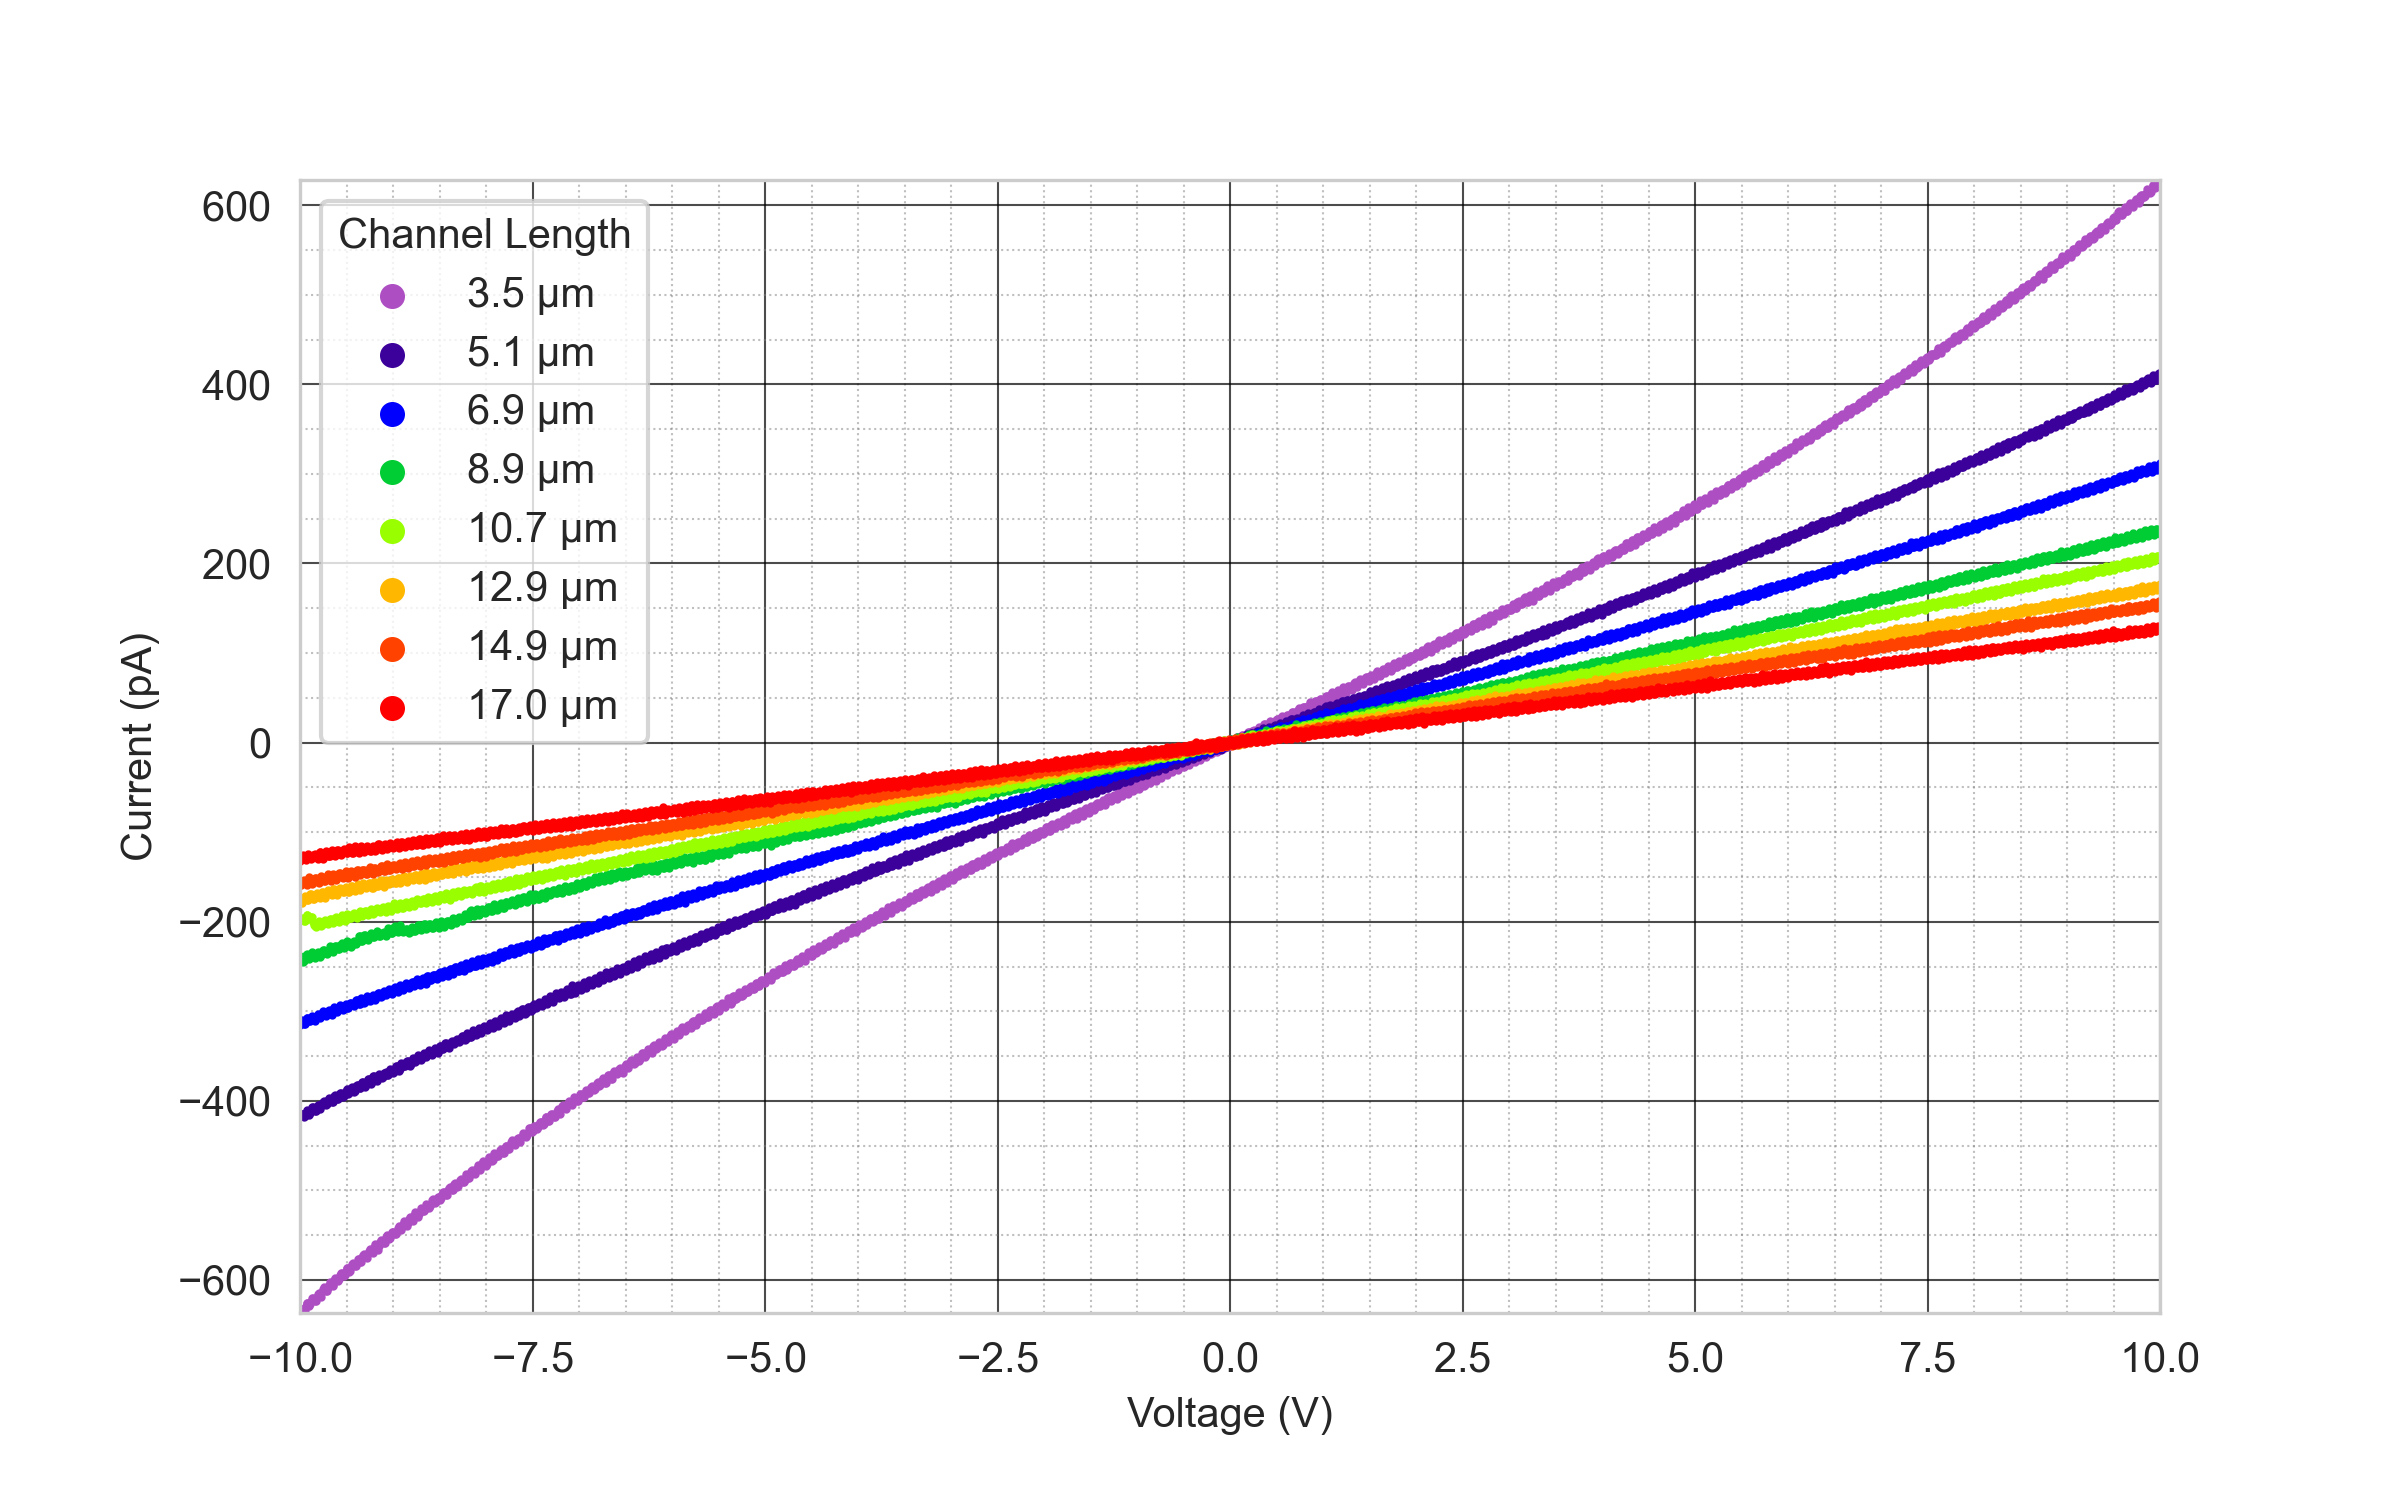
\includegraphics[width=0.97\textwidth]{Chapter3/Figs/Raster/Sample C 2019/IV/10V IV characteristics at 21 C.png}
    \caption{A linear plot of the measured current against applied voltage for all channel lengths at 21\si{\degreeCelsius} (sample C).}
    \label{appfig:C_current_voltage_21}
\end{figure}
\begin{figure}[h]
    \centering
    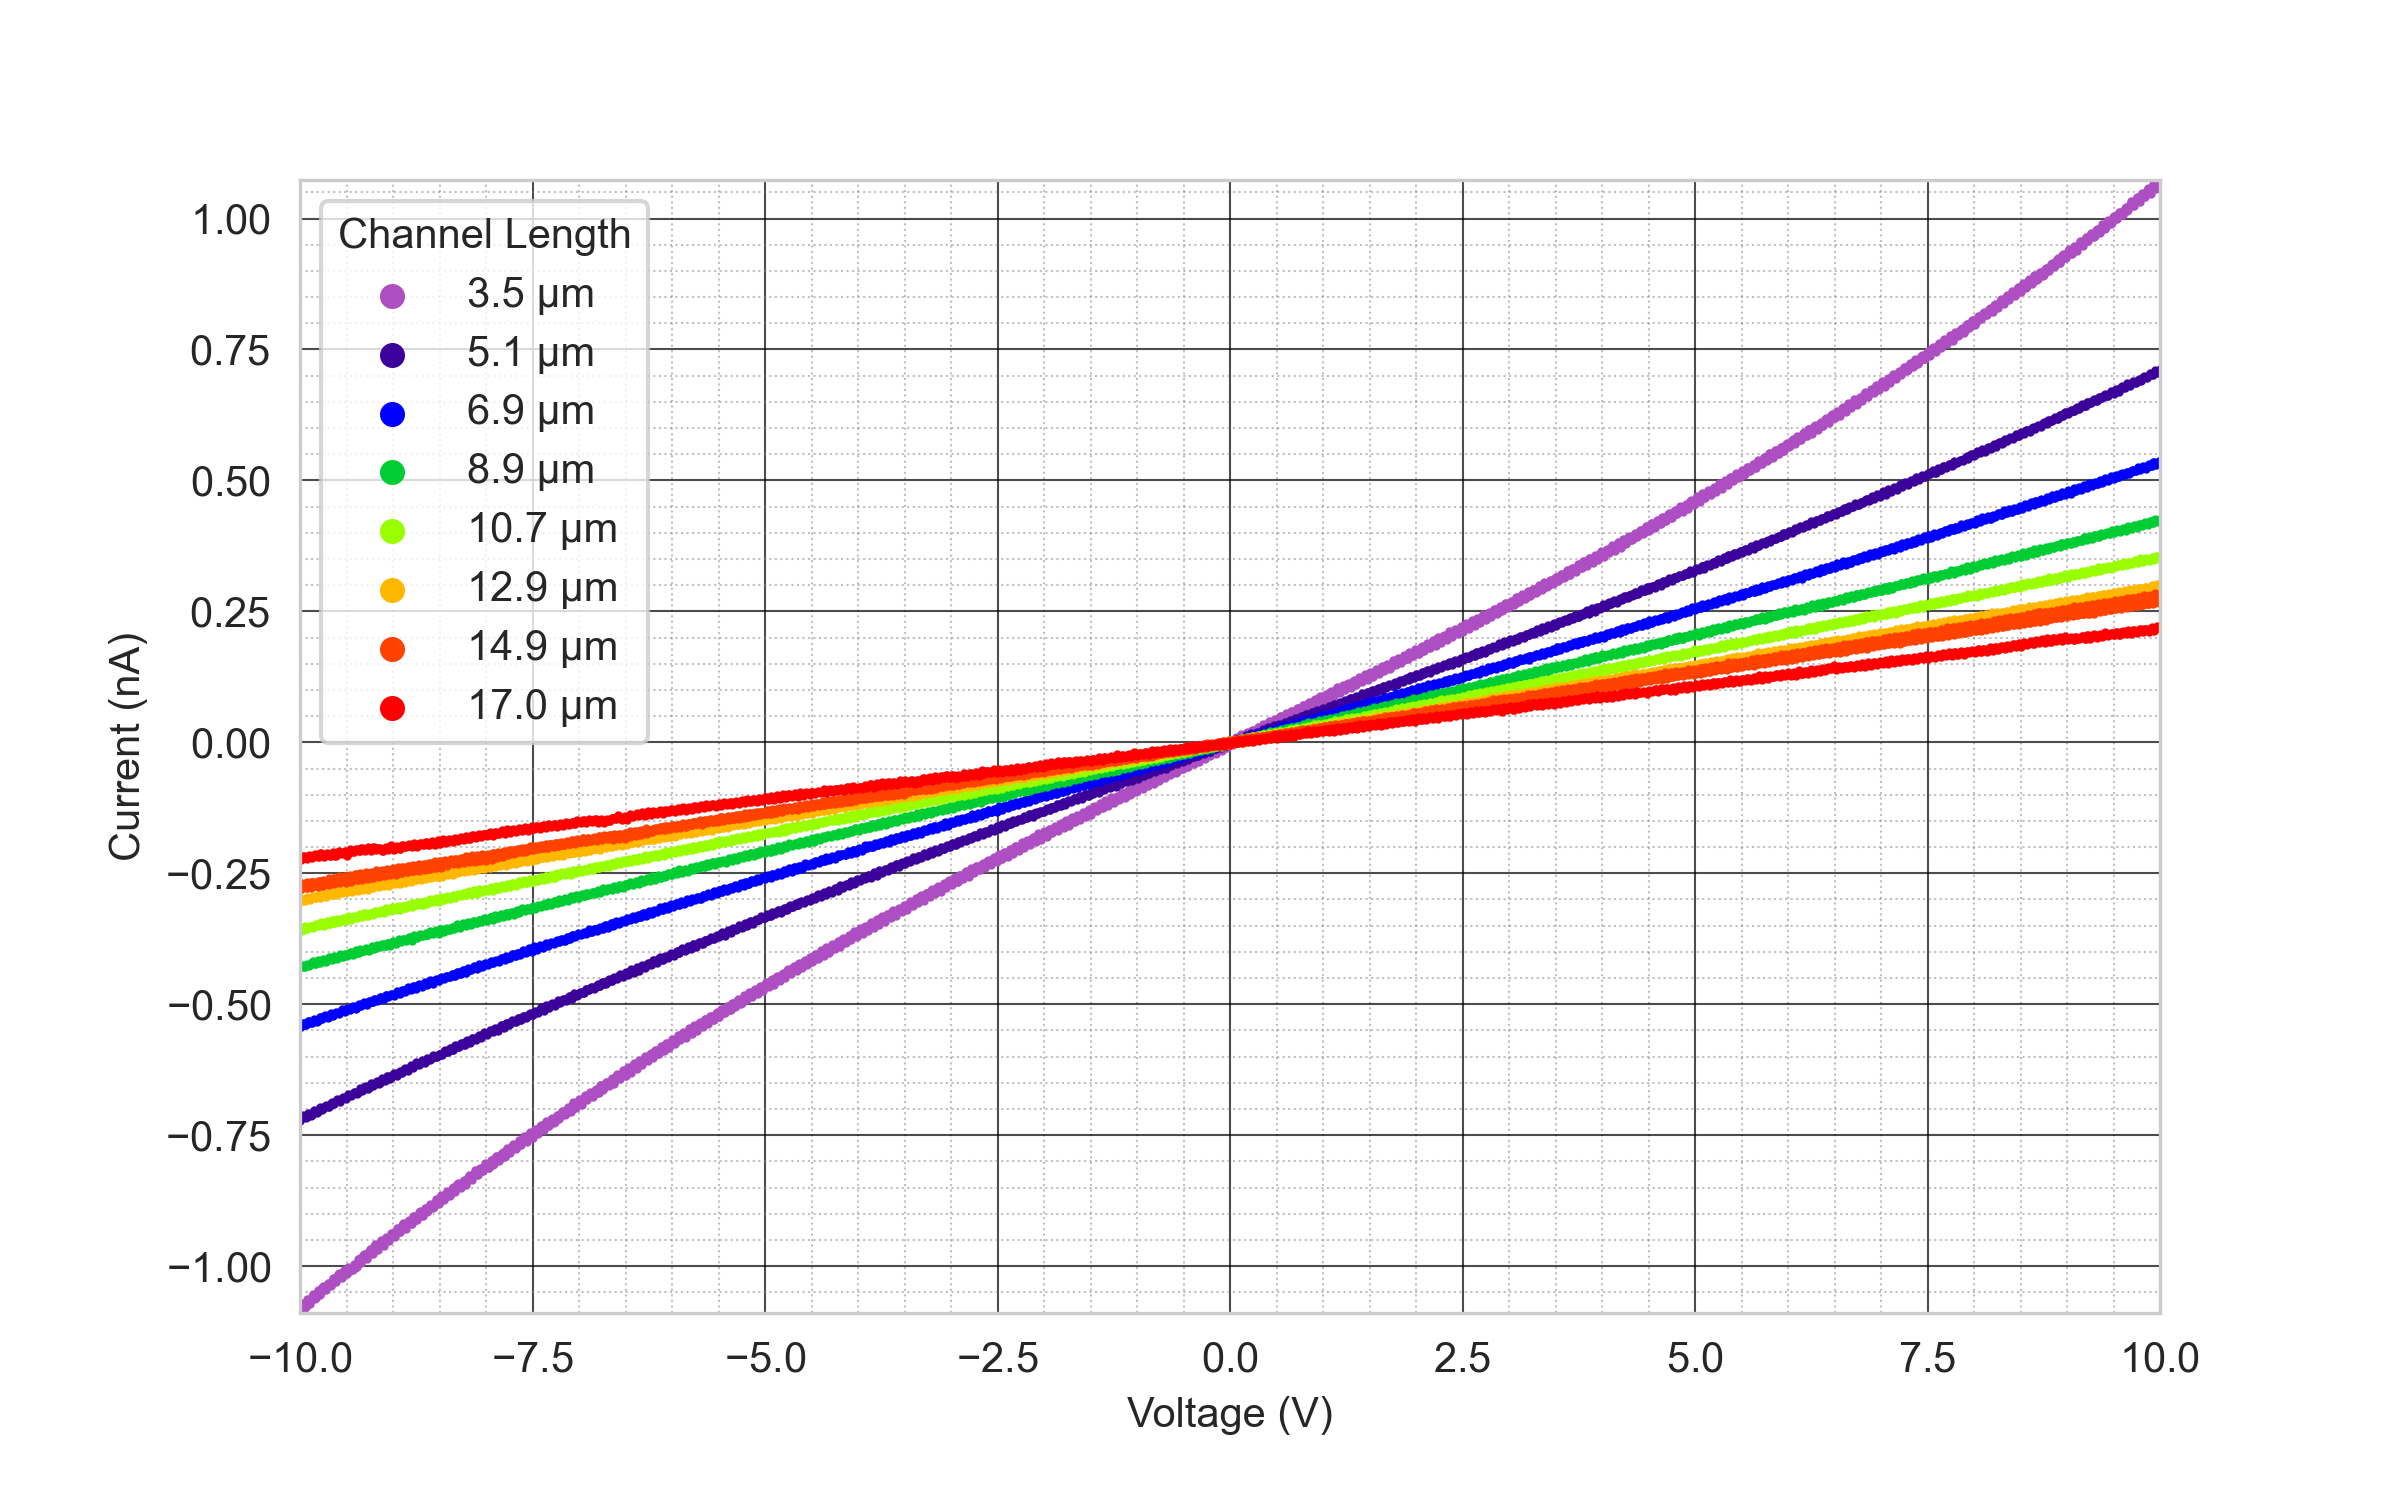
\includegraphics[width=0.97\textwidth]{Chapter3/Figs/Raster/Sample C 2019/IV/10V IV characteristics at 50 C.png}
    \caption{A linear plot of the measured current against applied voltage for all channel lengths at 50\si{\degreeCelsius} (sample C).}
    \label{appfig:C_current_voltage_50}
\end{figure}
\begin{figure}[h]
    \centering
    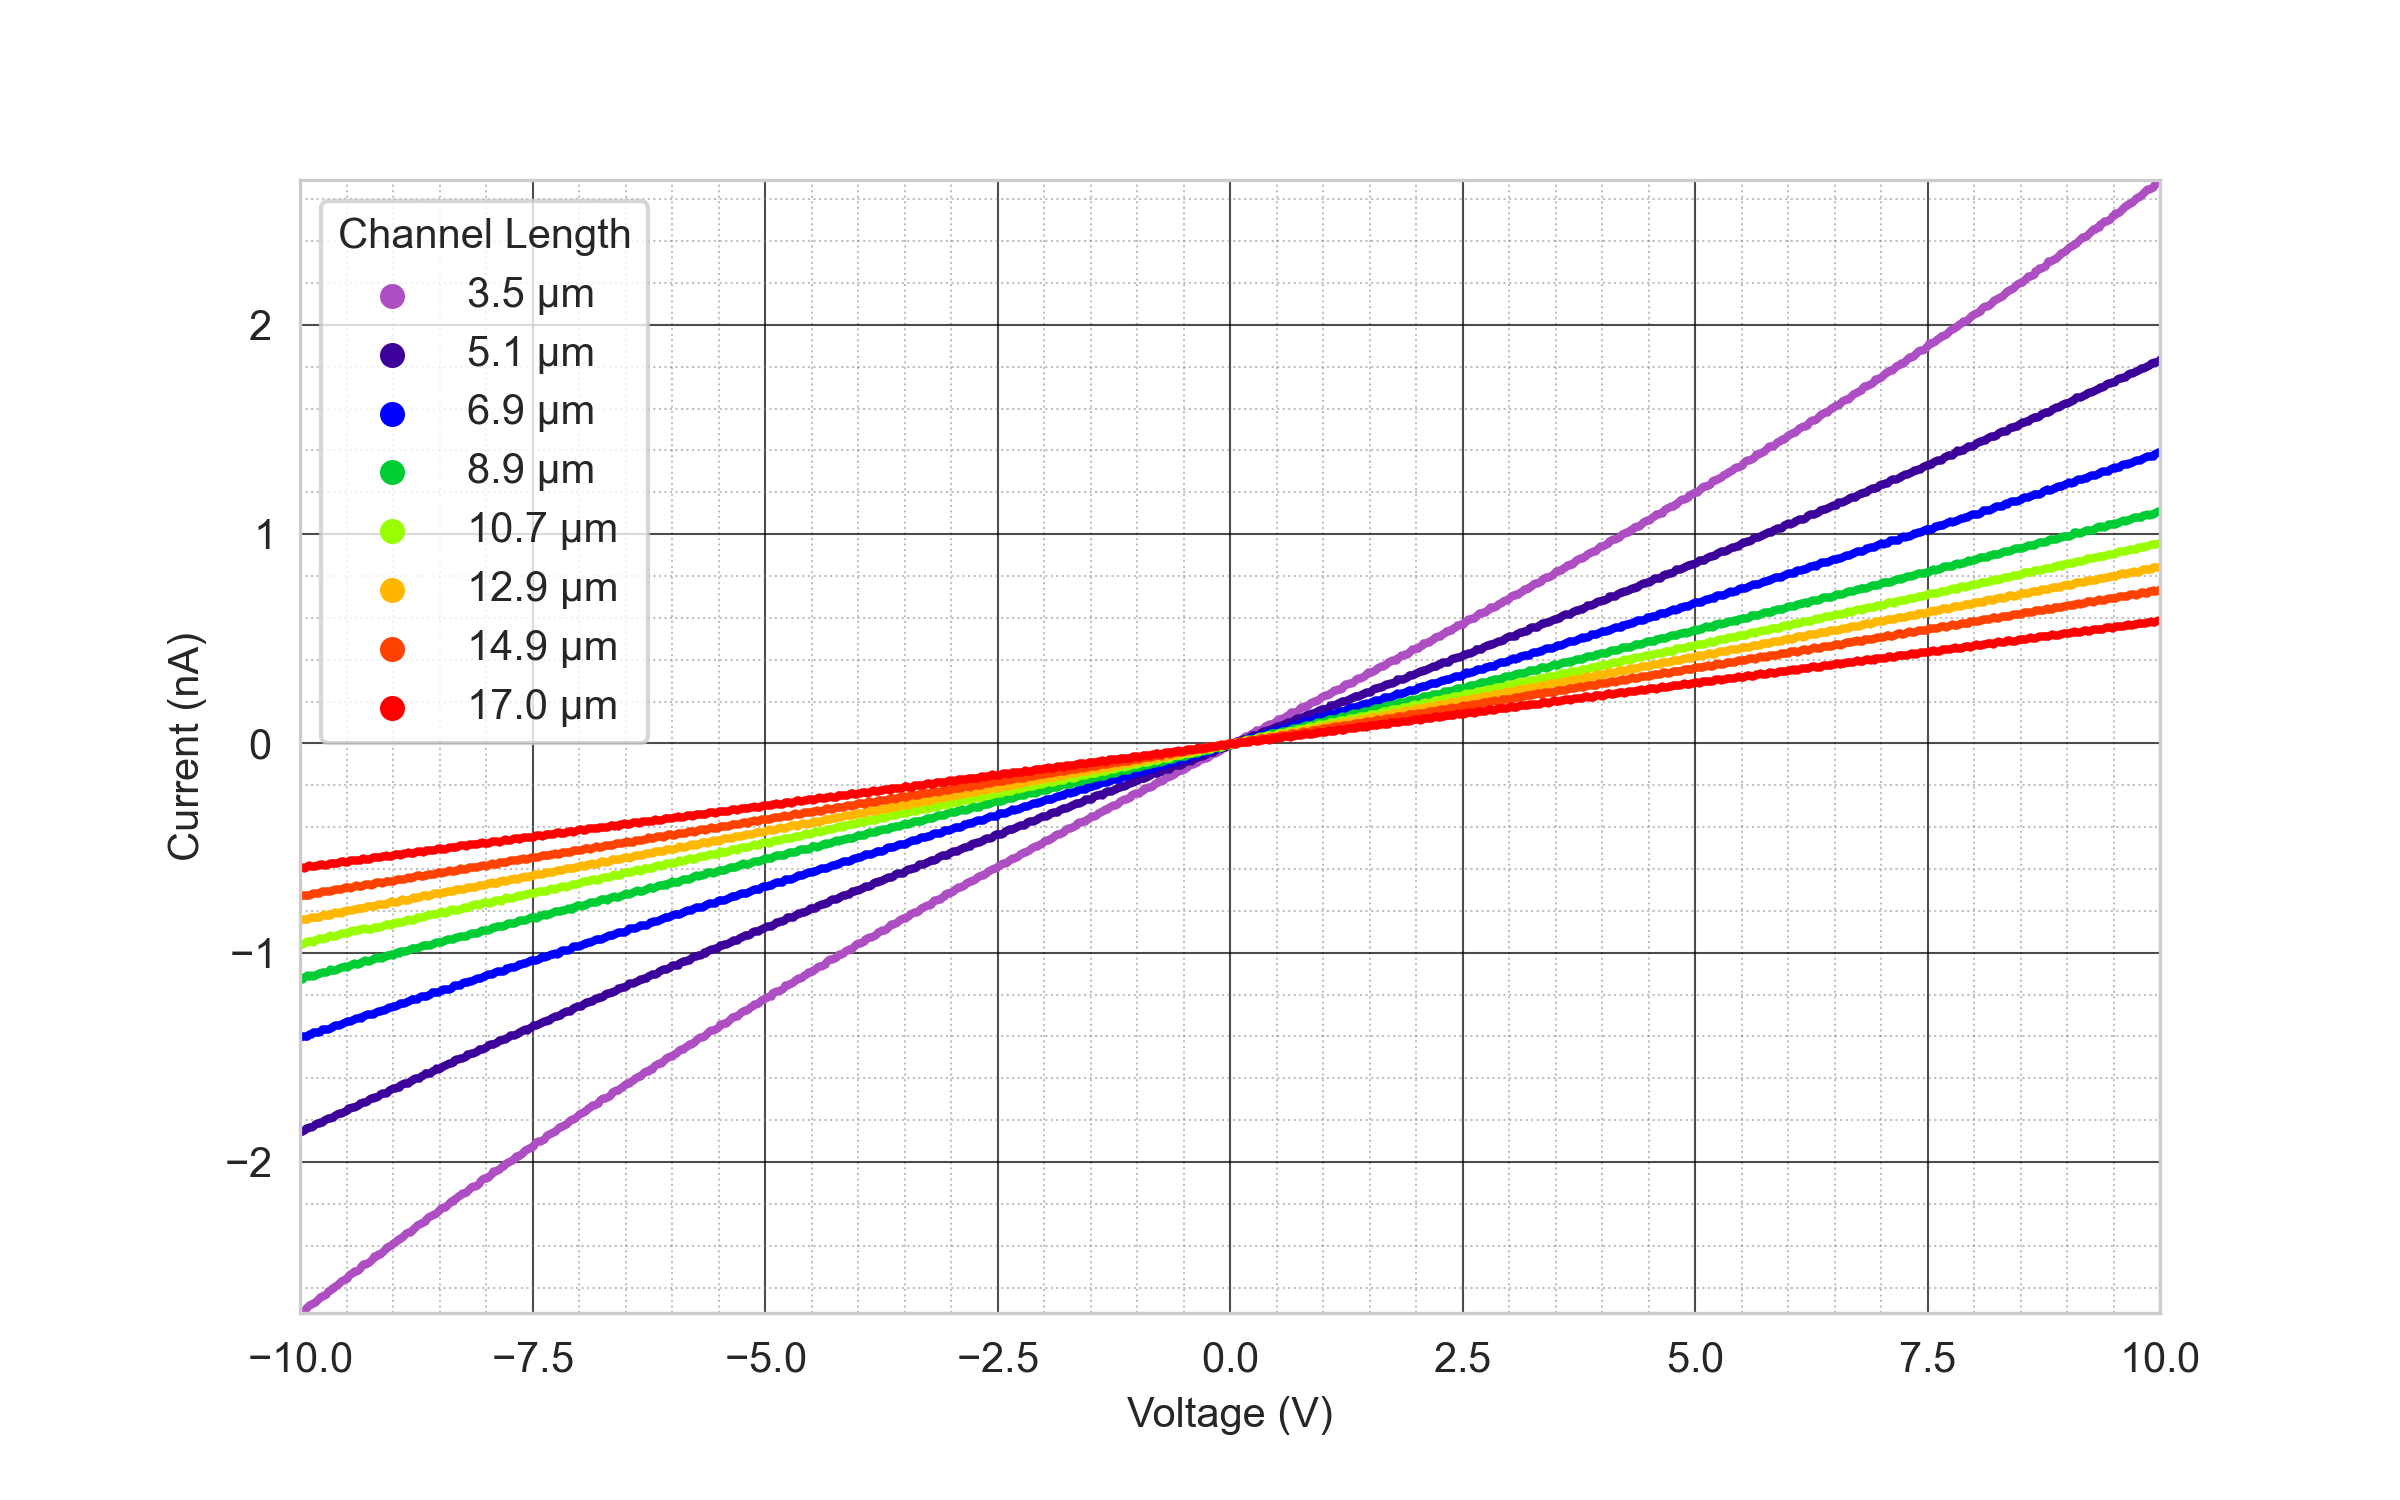
\includegraphics[width=0.97\textwidth]{Chapter3/Figs/Raster/Sample C 2019/IV/10V IV characteristics at 100 C.png}
    \caption{A linear plot of the measured current against applied voltage for all channel lengths at 100\si{\degreeCelsius} (sample C).}
    \label{appfig:C_current_voltage_100}
\end{figure}
\begin{figure}[h]
    \centering
    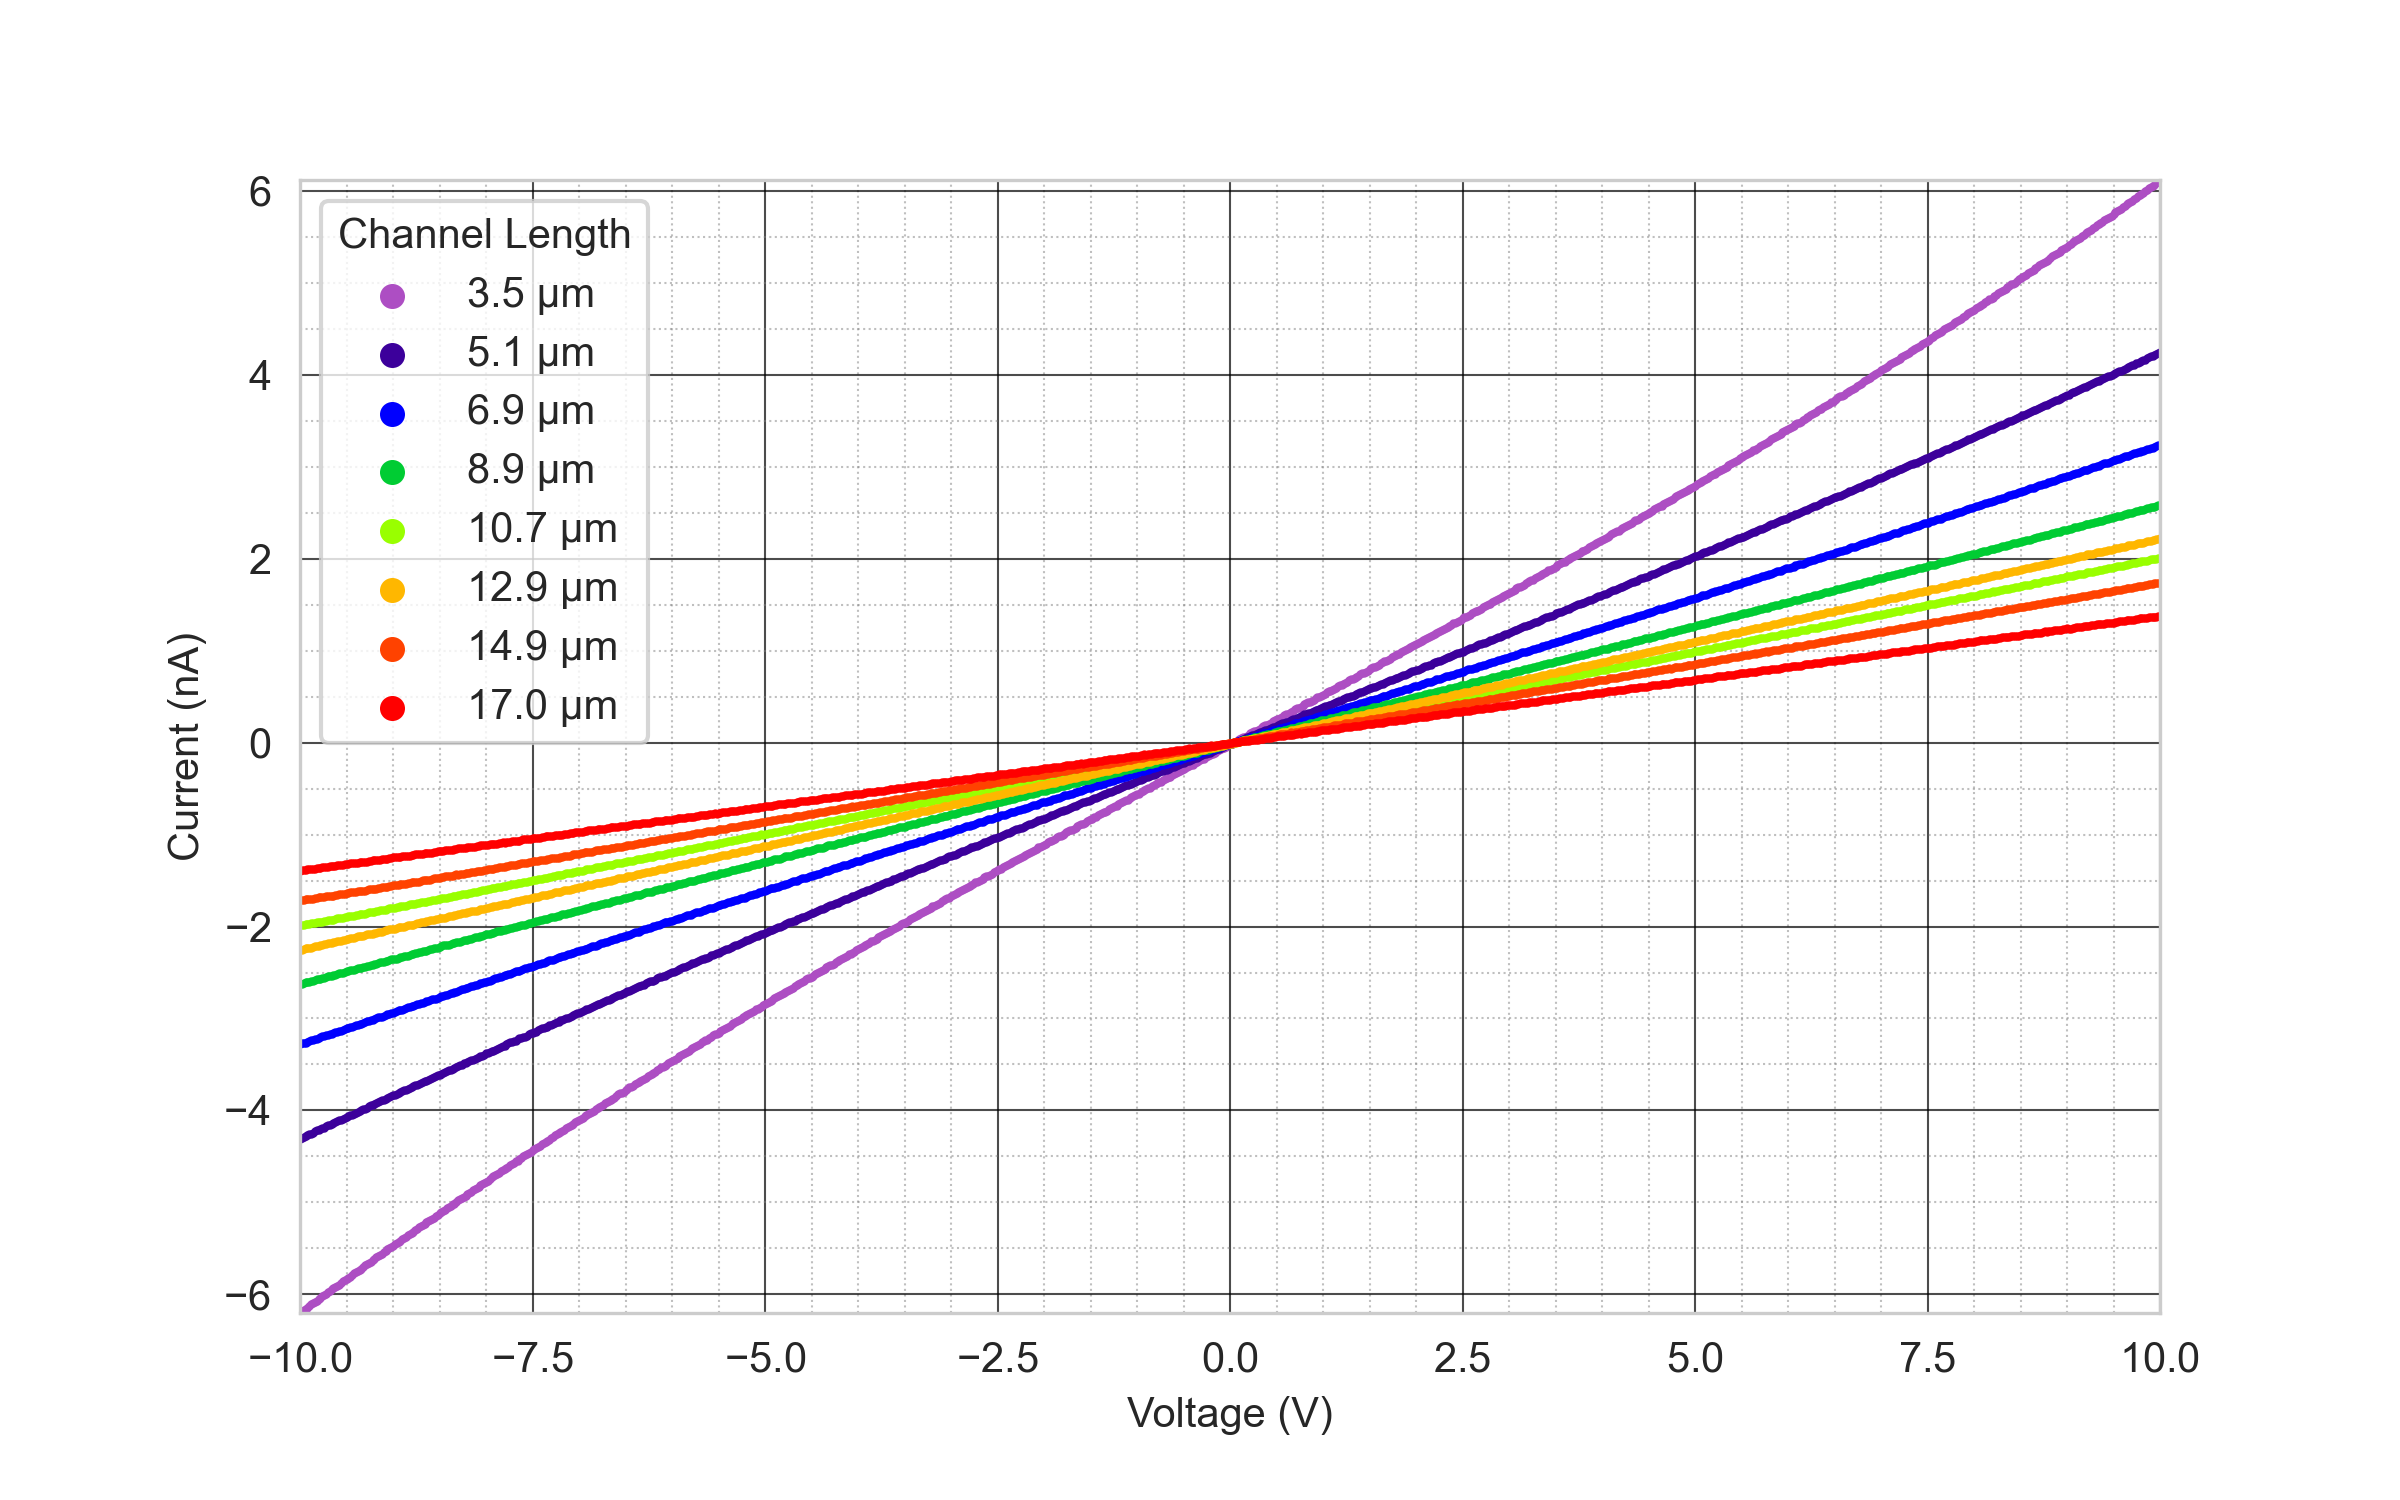
\includegraphics[width=0.97\textwidth]{Chapter3/Figs/Raster/Sample C 2019/IV/10V IV characteristics at 150 C.png}
    \caption{A linear plot of the measured current against applied voltage for all channel lengths at 150\si{\degreeCelsius} (sample C).}
    \label{appfig:C_current_voltage_150}
\end{figure}
\begin{figure}[h]
    \centering
    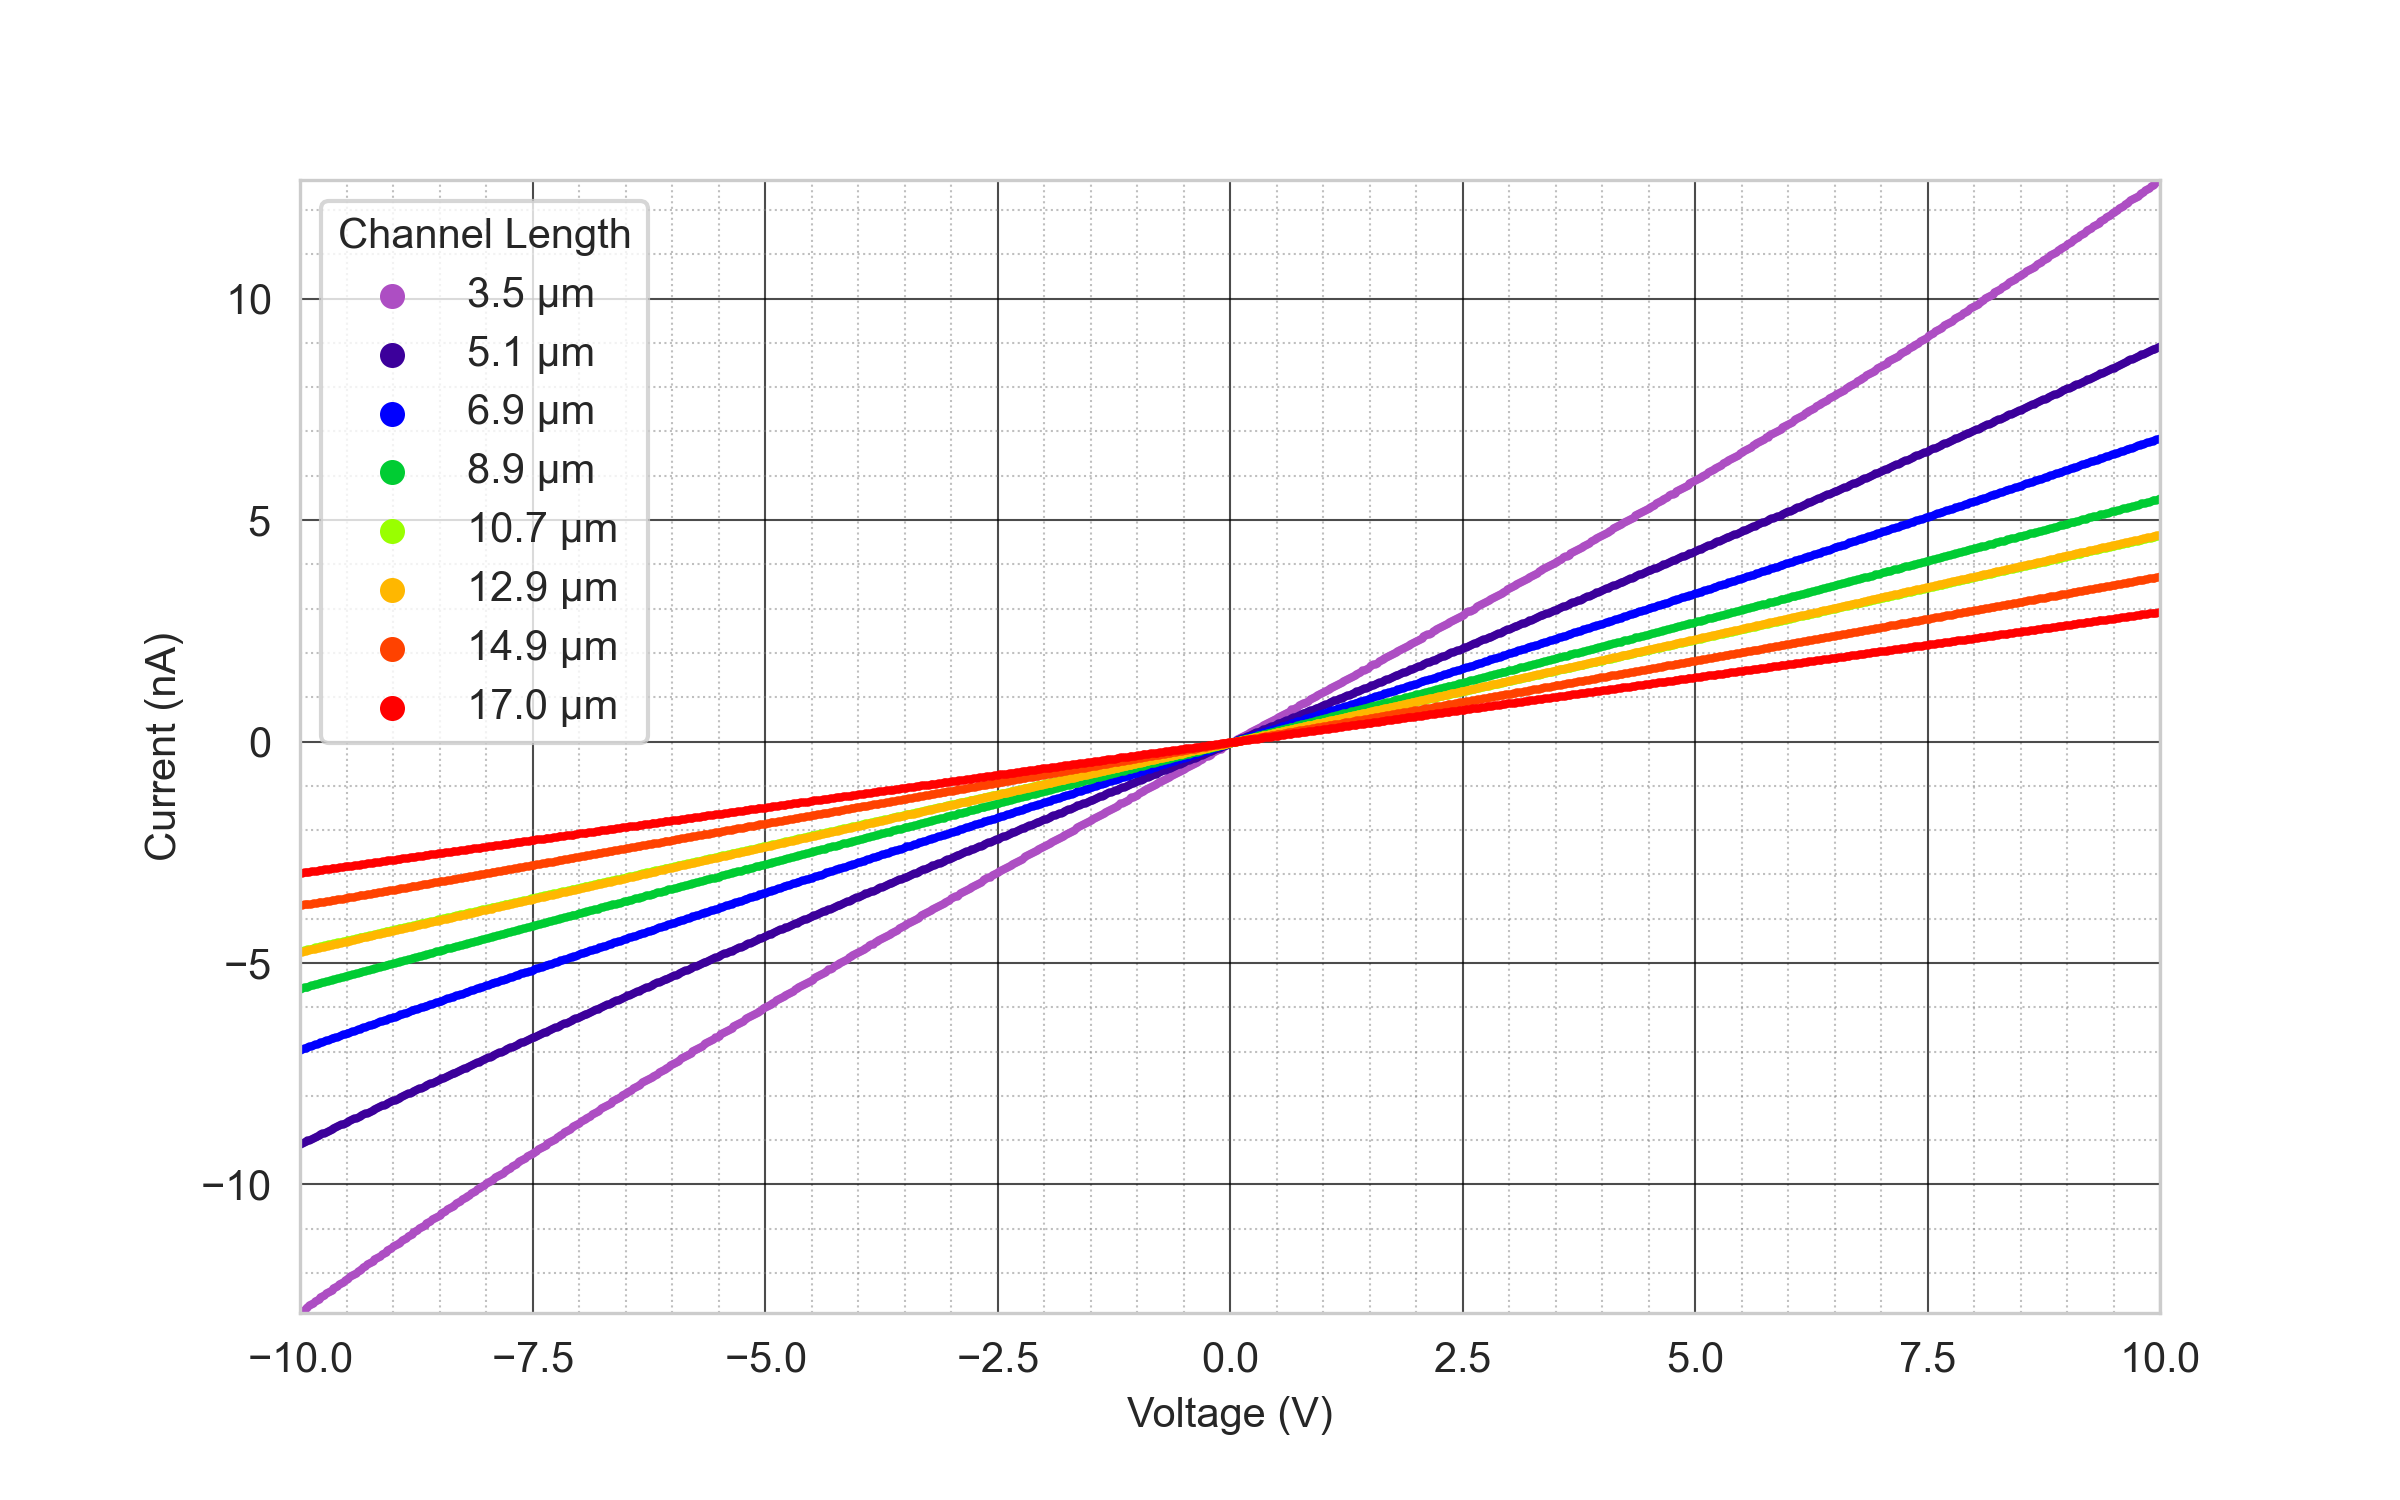
\includegraphics[width=0.97\textwidth]{Chapter3/Figs/Raster/Sample C 2019/IV/10V IV characteristics at 200 C.png}
    \caption{A linear plot of the measured current against applied voltage for all channel lengths at 200\si{\degreeCelsius} (sample C).}
    \label{appfig:C_current_voltage_200}
\end{figure}
\begin{figure}[h]
    \centering
    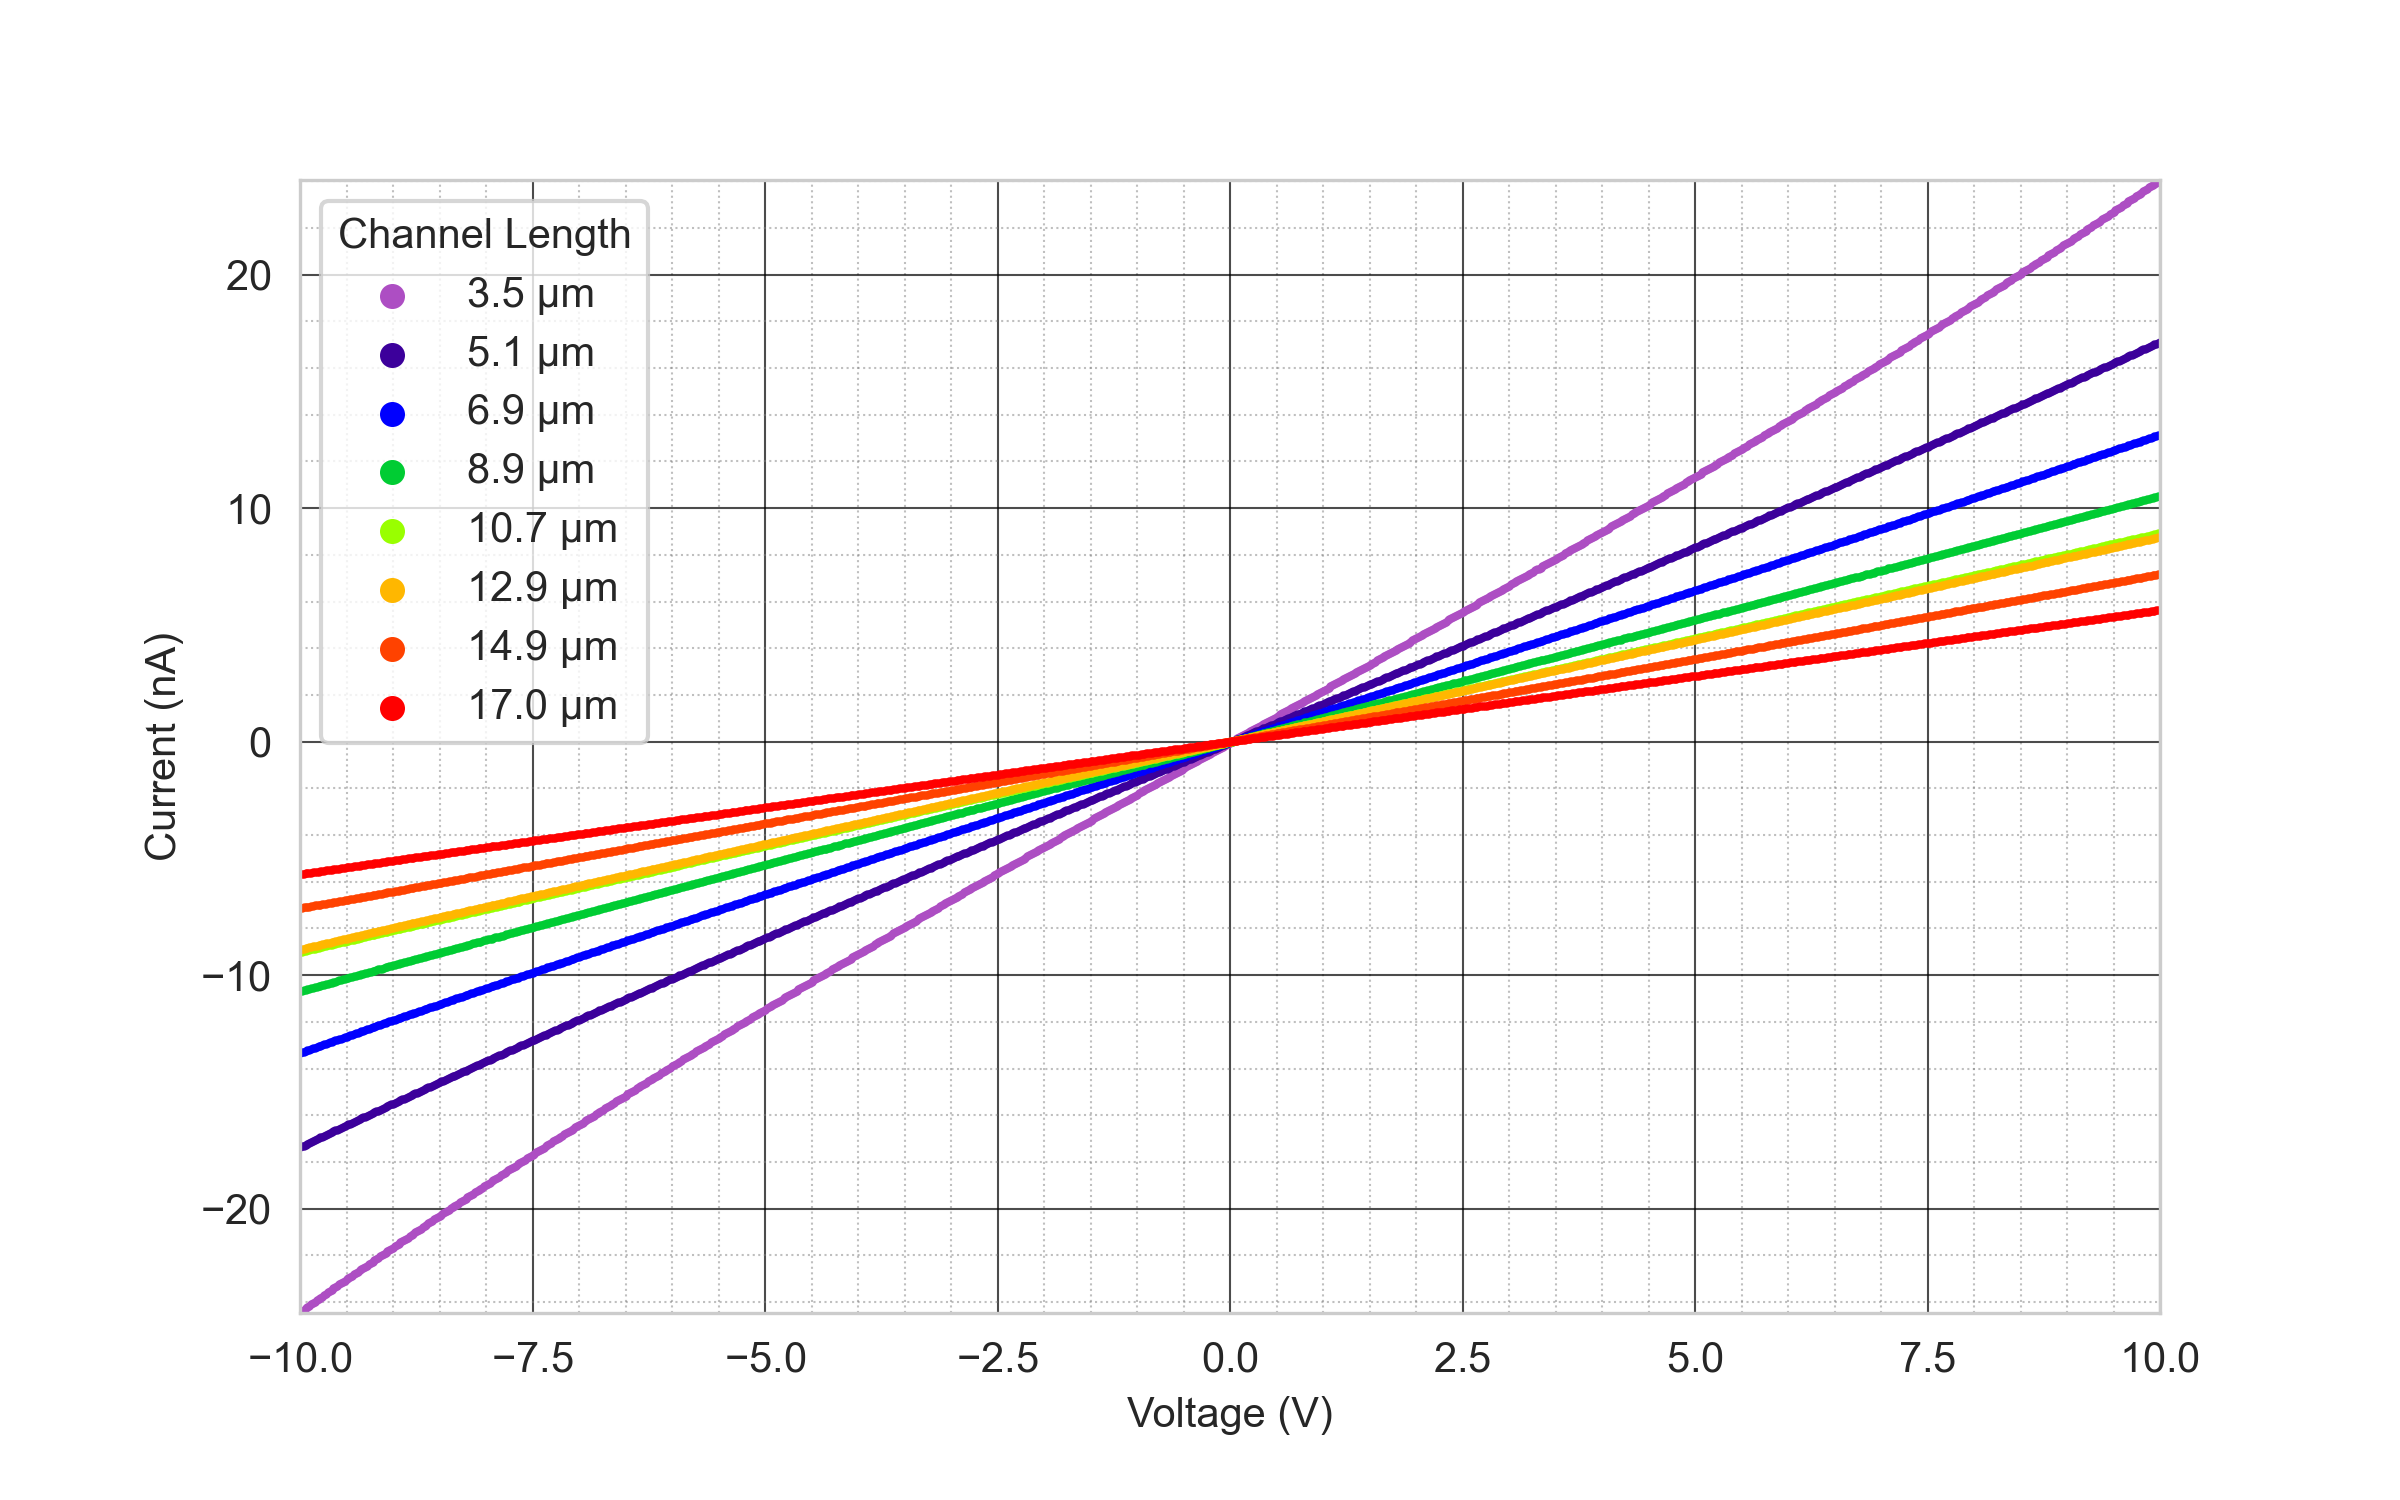
\includegraphics[width=0.97\textwidth]{Chapter3/Figs/Raster/Sample C 2019/IV/10V IV characteristics at 250 C.png}
    \caption{A linear plot of the measured current against applied voltage for all channel lengths at 250\si{\degreeCelsius} (sample C).}
    \label{appfig:C_current_voltage_250}
\end{figure}
\begin{figure}[h]
    \centering
    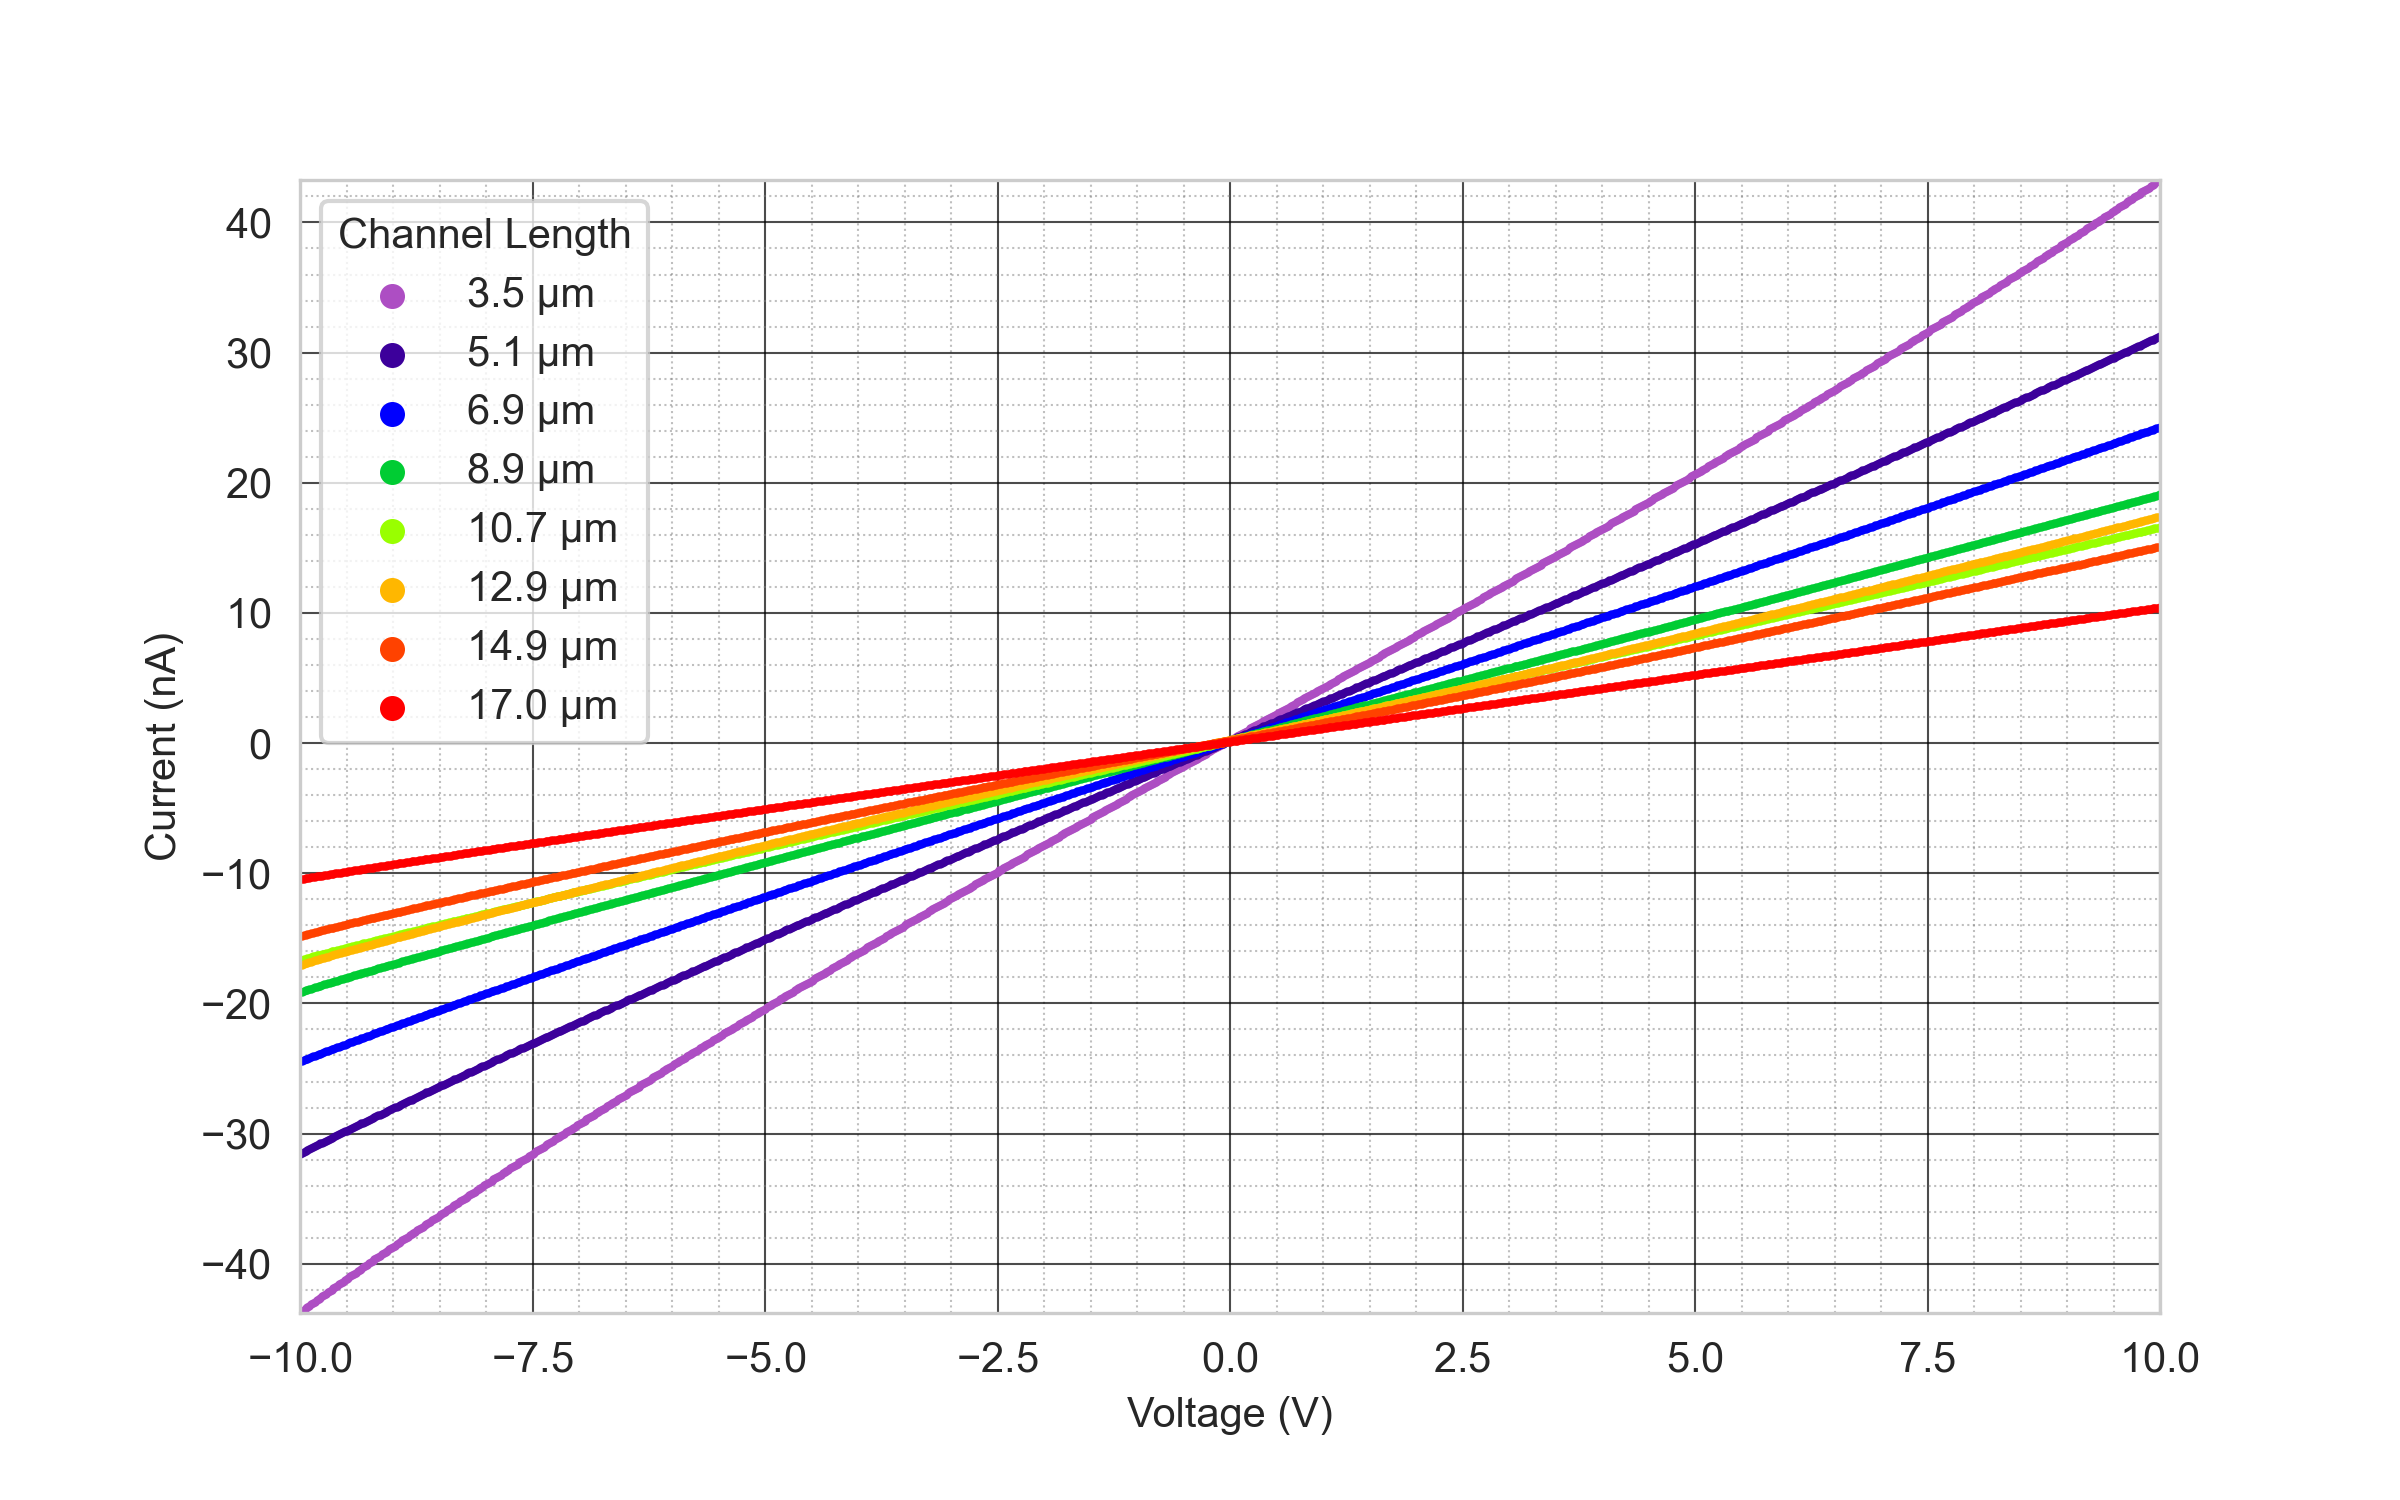
\includegraphics[width=0.97\textwidth]{Chapter3/Figs/Raster/Sample C 2019/IV/10V IV characteristics at 300 C.png}
    \caption{A linear plot of the measured current against applied voltage for all channel lengths at 300\si{\degreeCelsius} (sample C).}
    \label{appfig:C_current_voltage_300}
\end{figure}

\subsection{Sample D: 10 \si{\volt} range}

\label{app:I_V_sample_D_10V}
\begin{figure}[h]
    \centering
    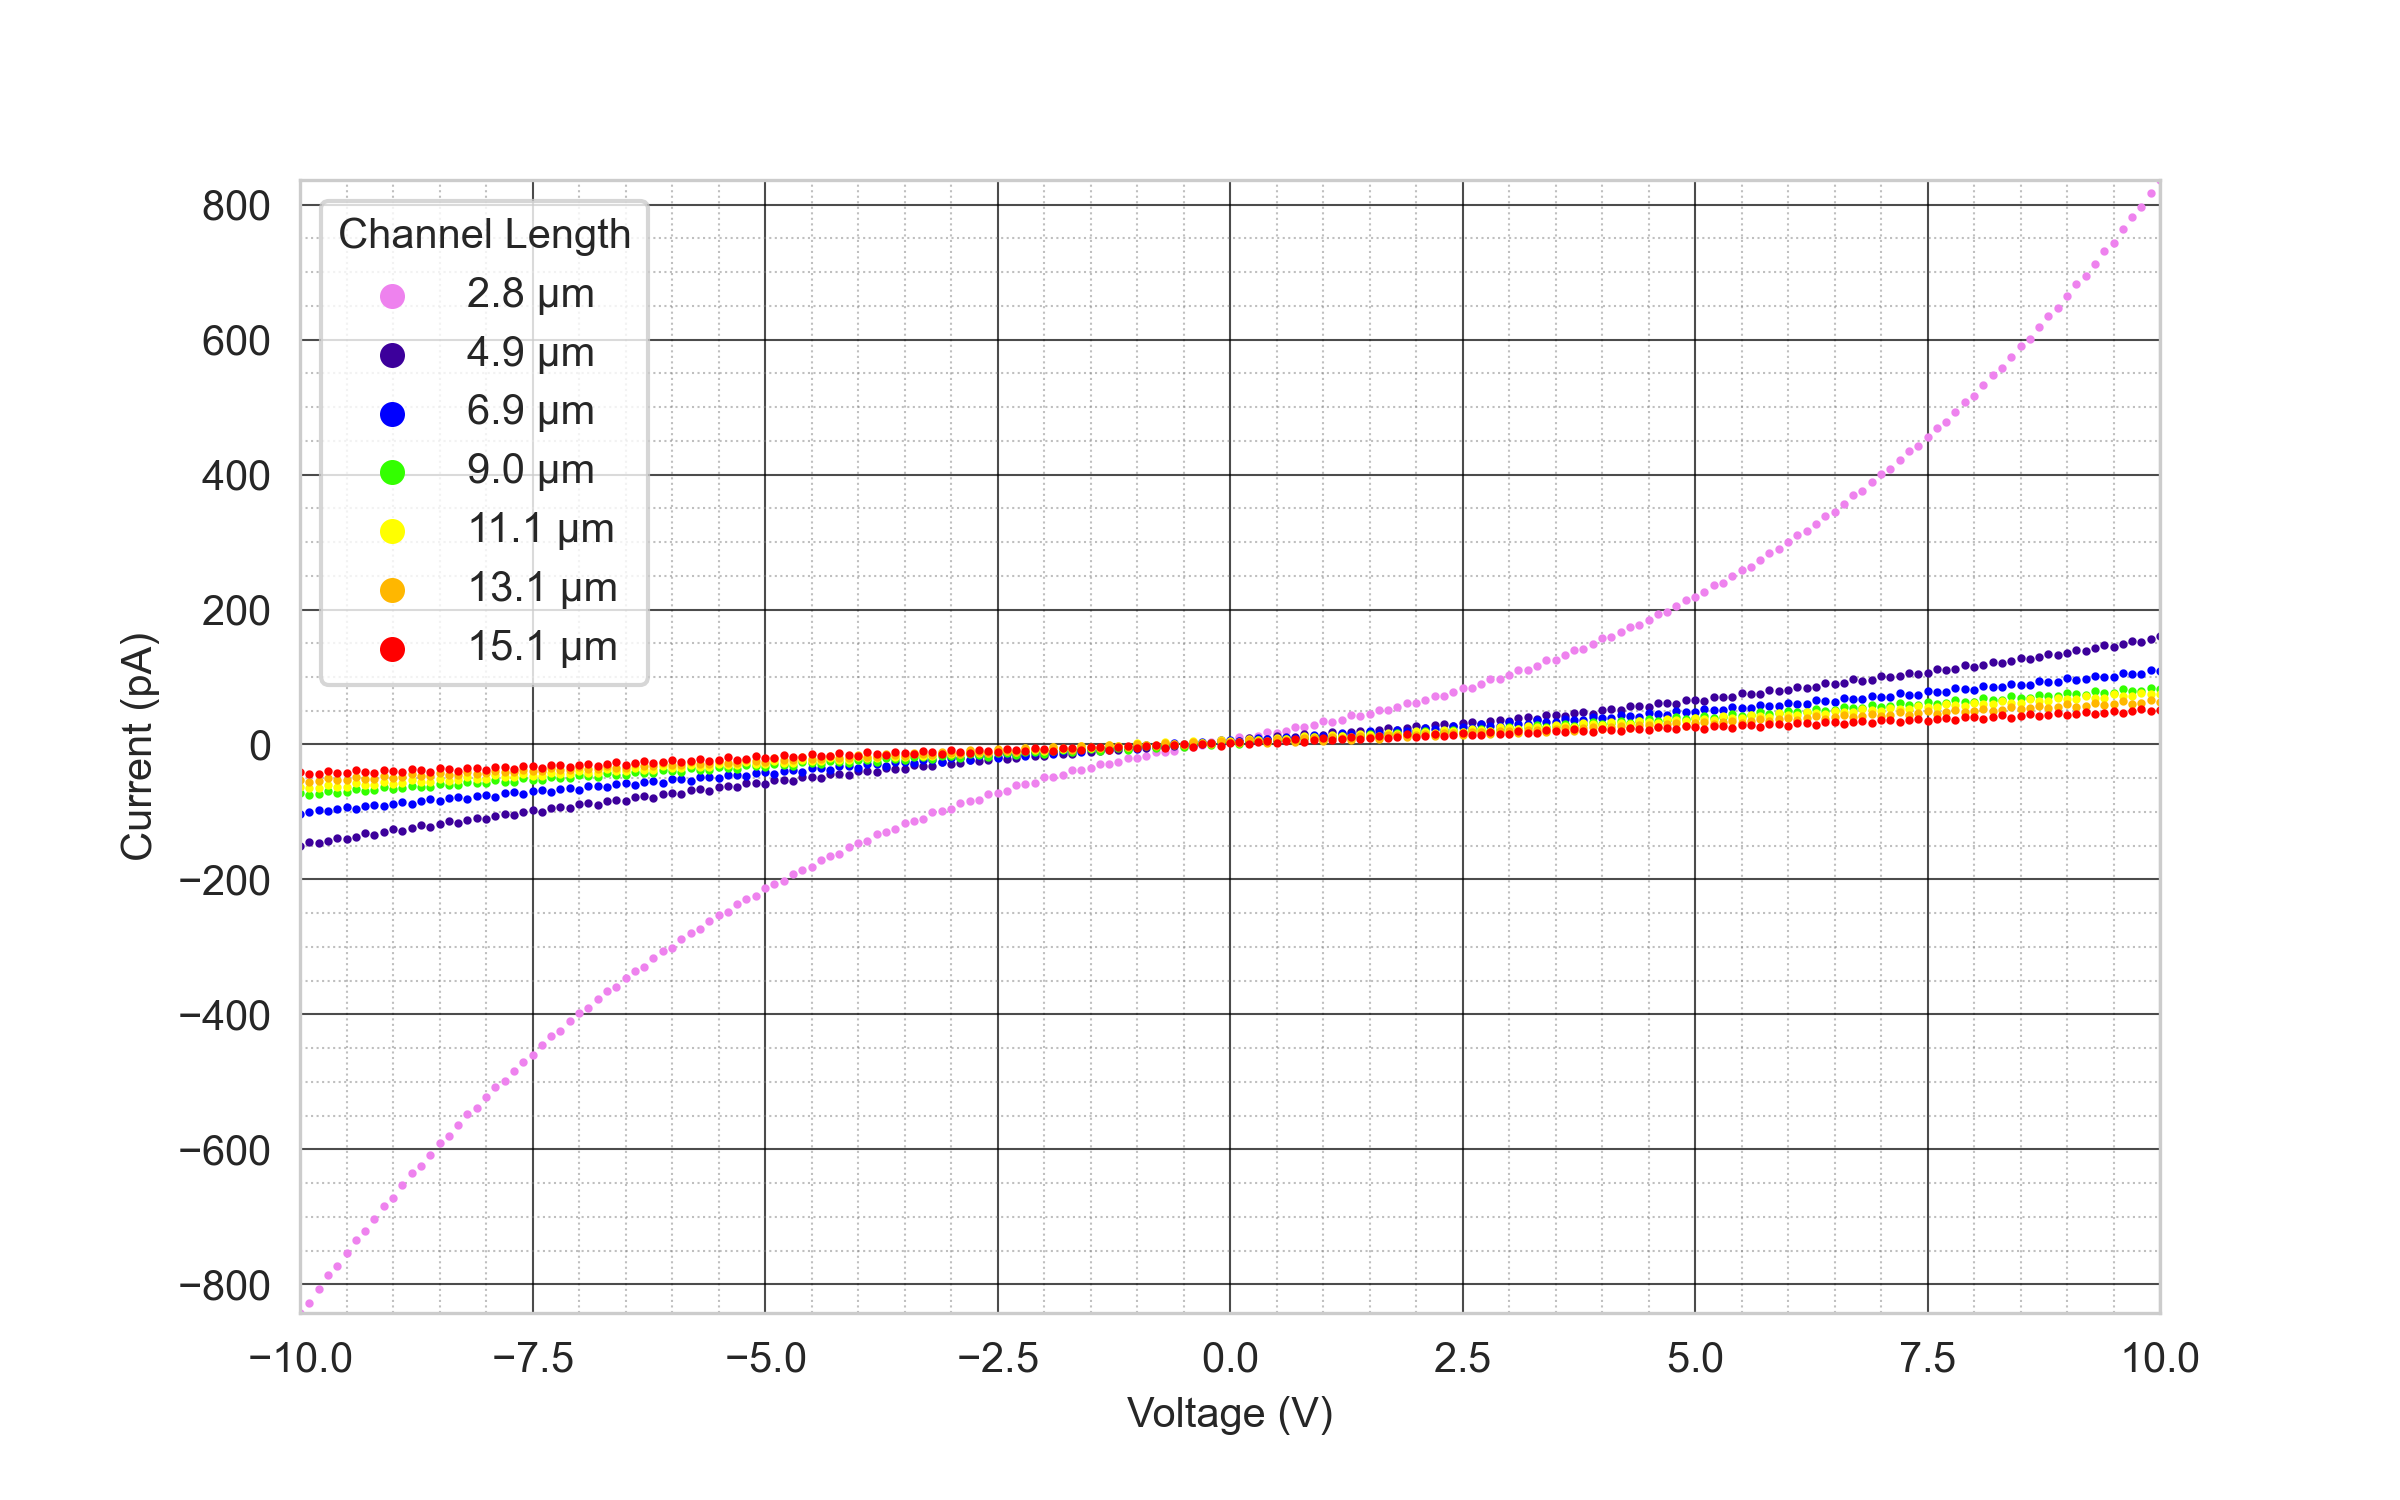
\includegraphics[width=0.97\textwidth]{Chapter3/Figs/Raster/Sample D 2019/IV/10V IV characteristics at 21 C.png}
    \caption{A linear plot of the measured current against applied voltage for all channel lengths at 21\si{\degreeCelsius} (sample D).}
    \label{appfig:D_current_voltage_21_10V}
\end{figure}
\begin{figure}[h]
    \centering
    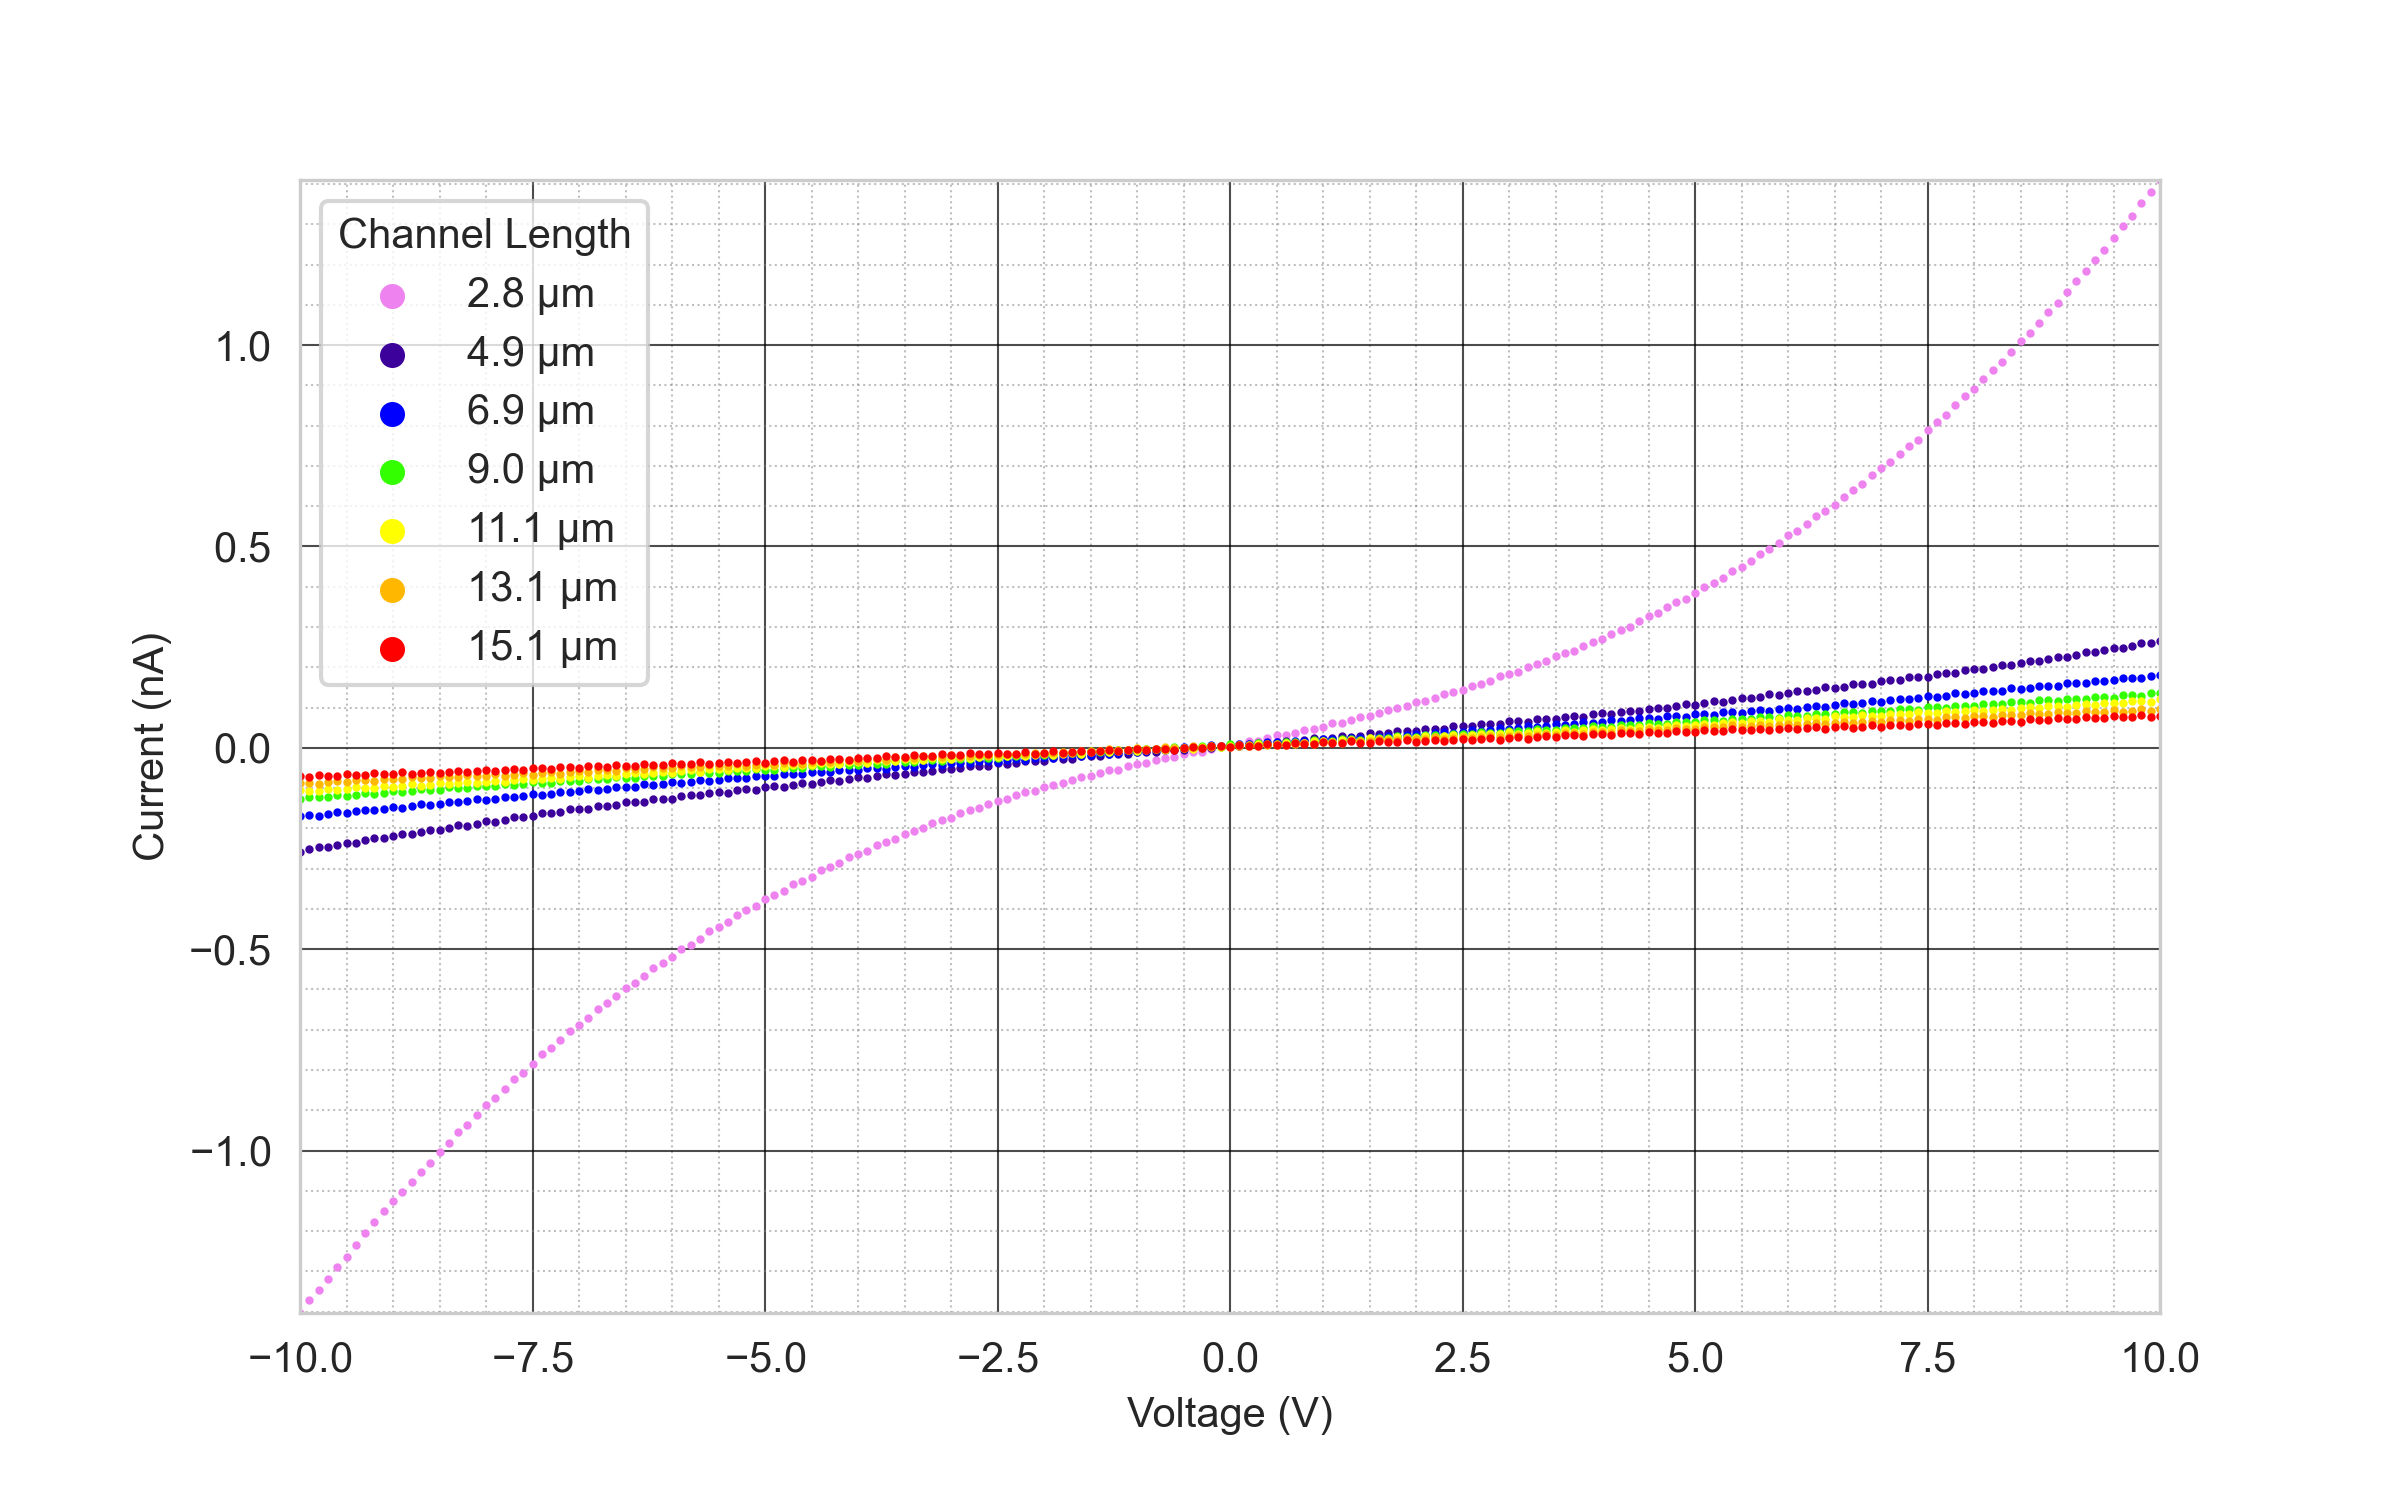
\includegraphics[width=0.97\textwidth]{Chapter3/Figs/Raster/Sample D 2019/IV/10V IV characteristics at 50 C.png}
    \caption{A linear plot of the measured current against applied voltage for all channel lengths at 50\si{\degreeCelsius} (sample D).}
    \label{appfig:D_current_voltage_50_10V}
\end{figure}
\begin{figure}[h]
    \centering
    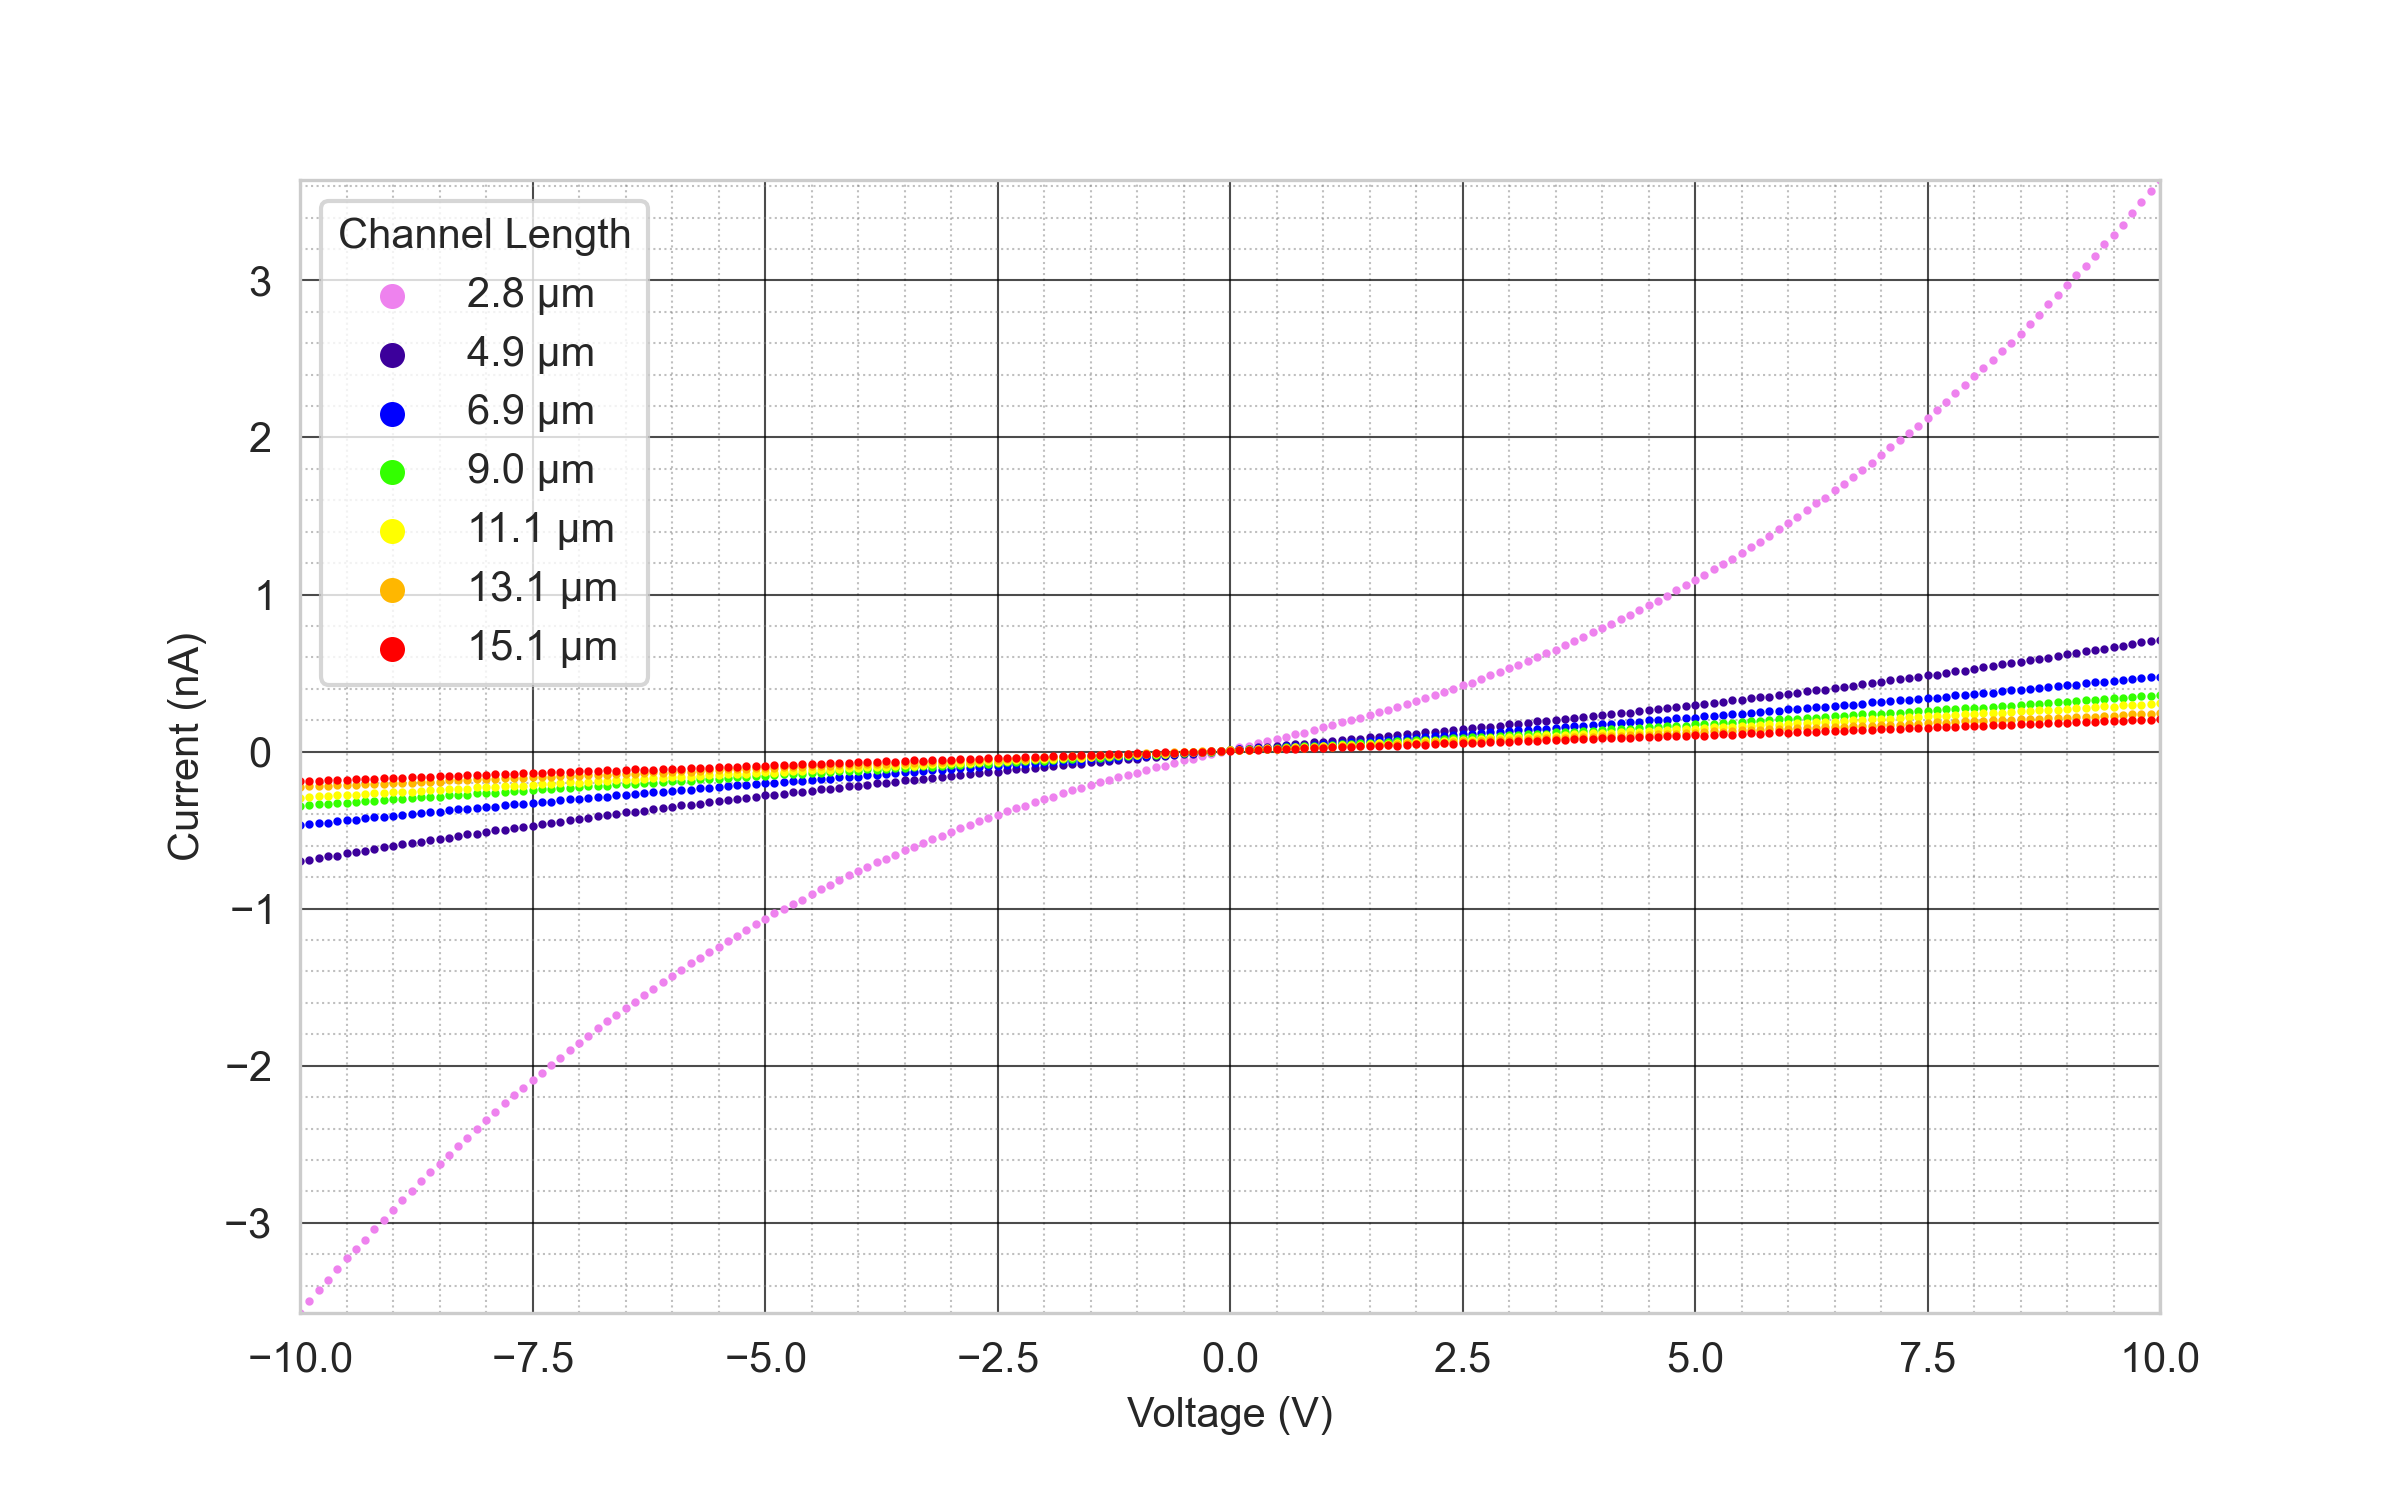
\includegraphics[width=0.97\textwidth]{Chapter3/Figs/Raster/Sample D 2019/IV/10V IV characteristics at 100 C.png}
    \caption{A linear plot of the measured current against applied voltage for all channel lengths at 100\si{\degreeCelsius} (sample D).}
    \label{appfig:D_current_voltage_100_10V}
\end{figure}
\begin{figure}[h]
    \centering
    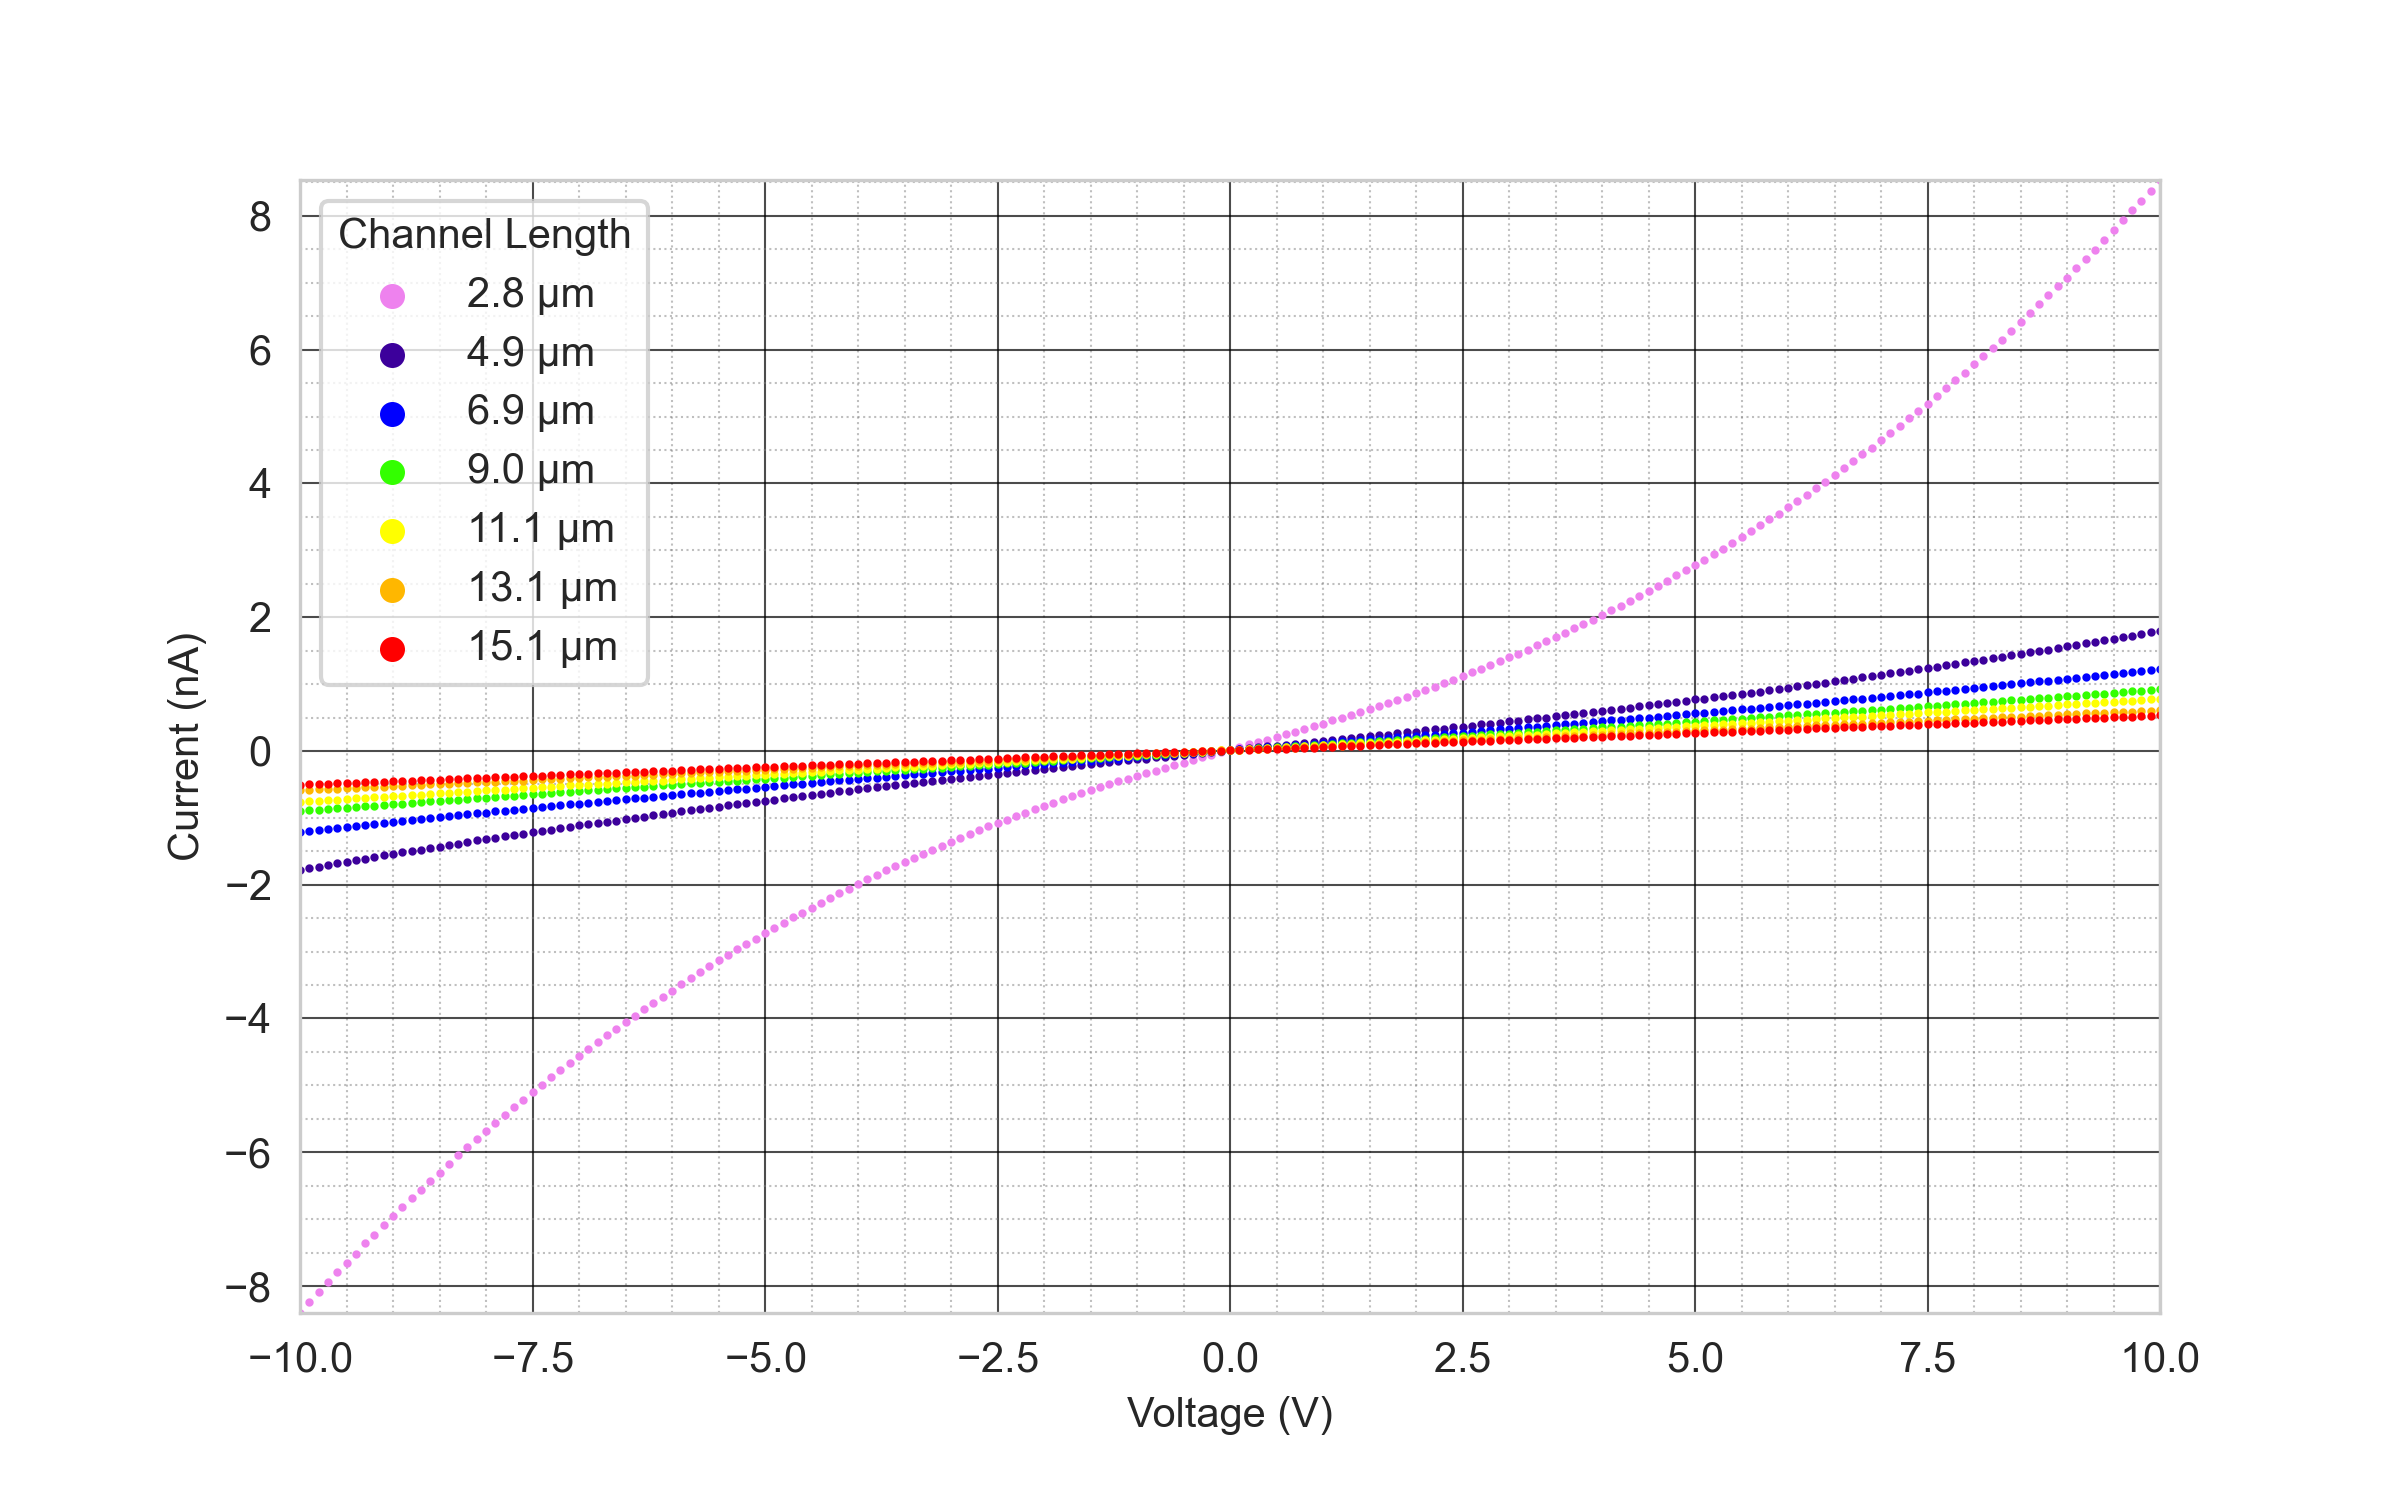
\includegraphics[width=0.97\textwidth]{Chapter3/Figs/Raster/Sample D 2019/IV/10V IV characteristics at 150 C.png}
    \caption{A linear plot of the measured current against applied voltage for all channel lengths at 150\si{\degreeCelsius} (sample D).}
    \label{appfig:D_current_voltage_150_10V}
\end{figure}
\begin{figure}[h]
    \centering
    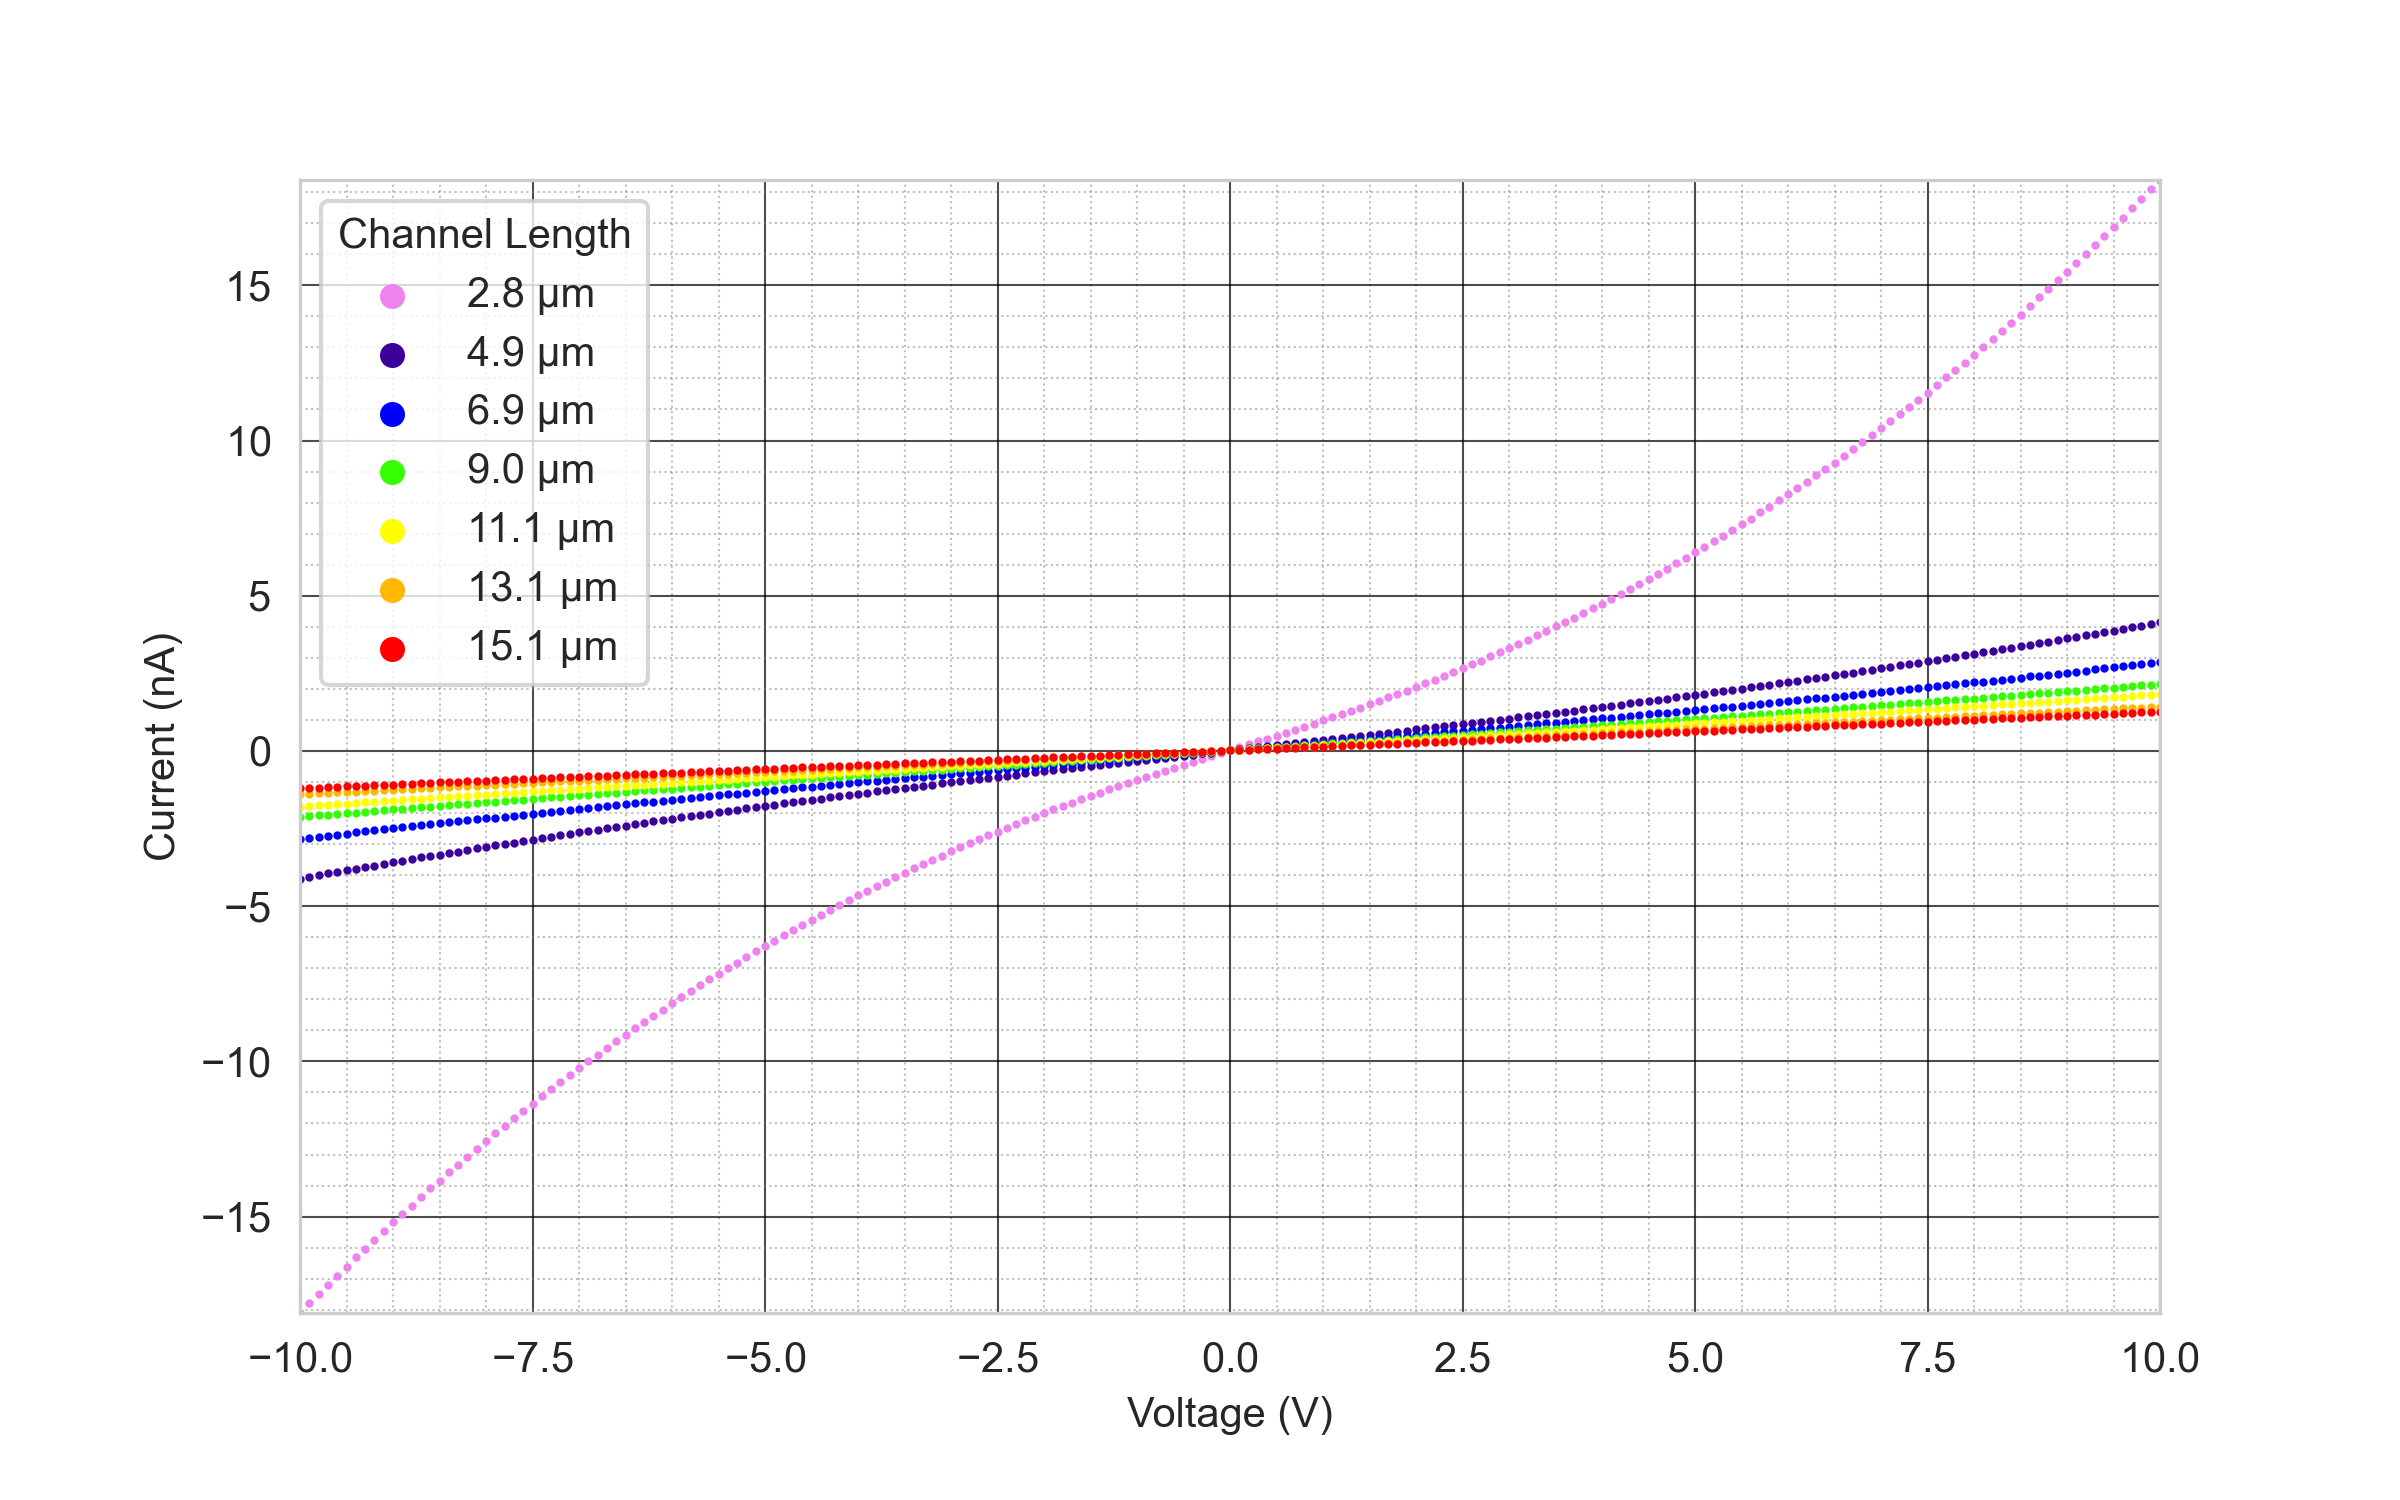
\includegraphics[width=0.97\textwidth]{Chapter3/Figs/Raster/Sample D 2019/IV/10V IV characteristics at 200 C.png}
    \caption{A linear plot of the measured current against applied voltage for all channel lengths at 200\si{\degreeCelsius} (sample D).}
    \label{appfig:D_current_voltage_200_10V}
\end{figure}
\begin{figure}[h]
    \centering
    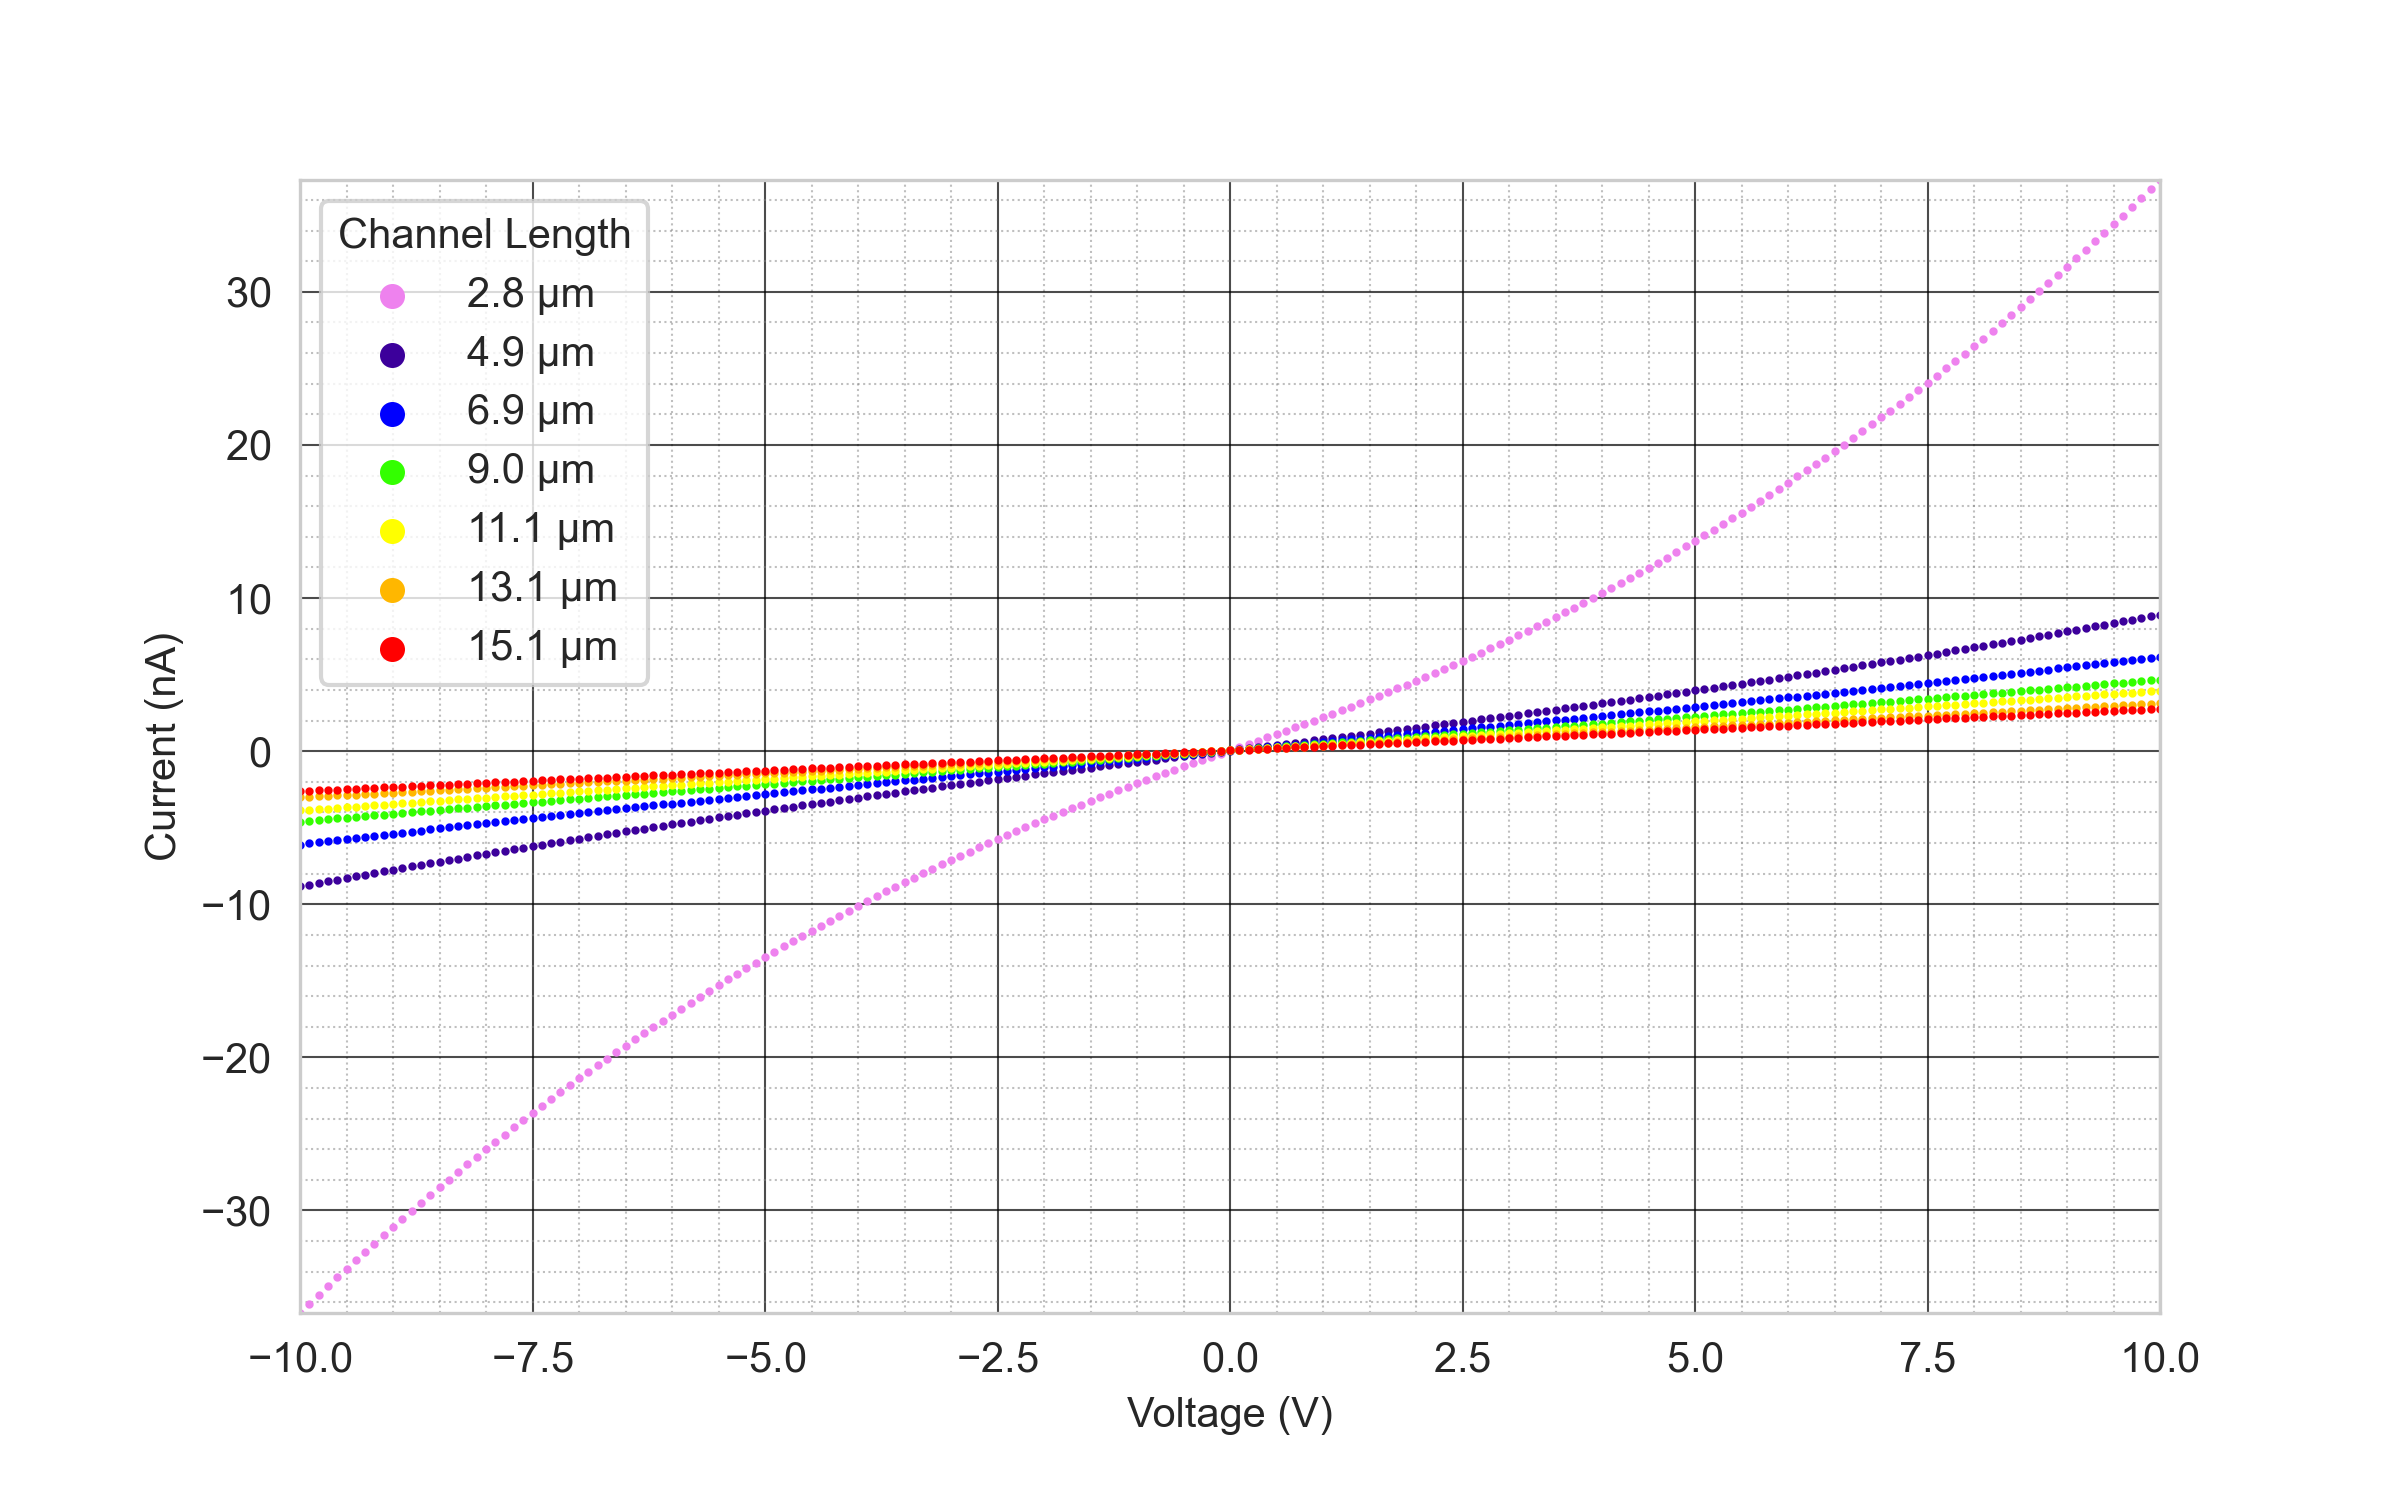
\includegraphics[width=0.97\textwidth]{Chapter3/Figs/Raster/Sample D 2019/IV/10V IV characteristics at 250 C.png}
    \caption{A linear plot of the measured current against applied voltage for all channel lengths at 250\si{\degreeCelsius} (sample D).}
    \label{appfig:D_current_voltage_250_10V}
\end{figure}
\begin{figure}[h]
    \centering
    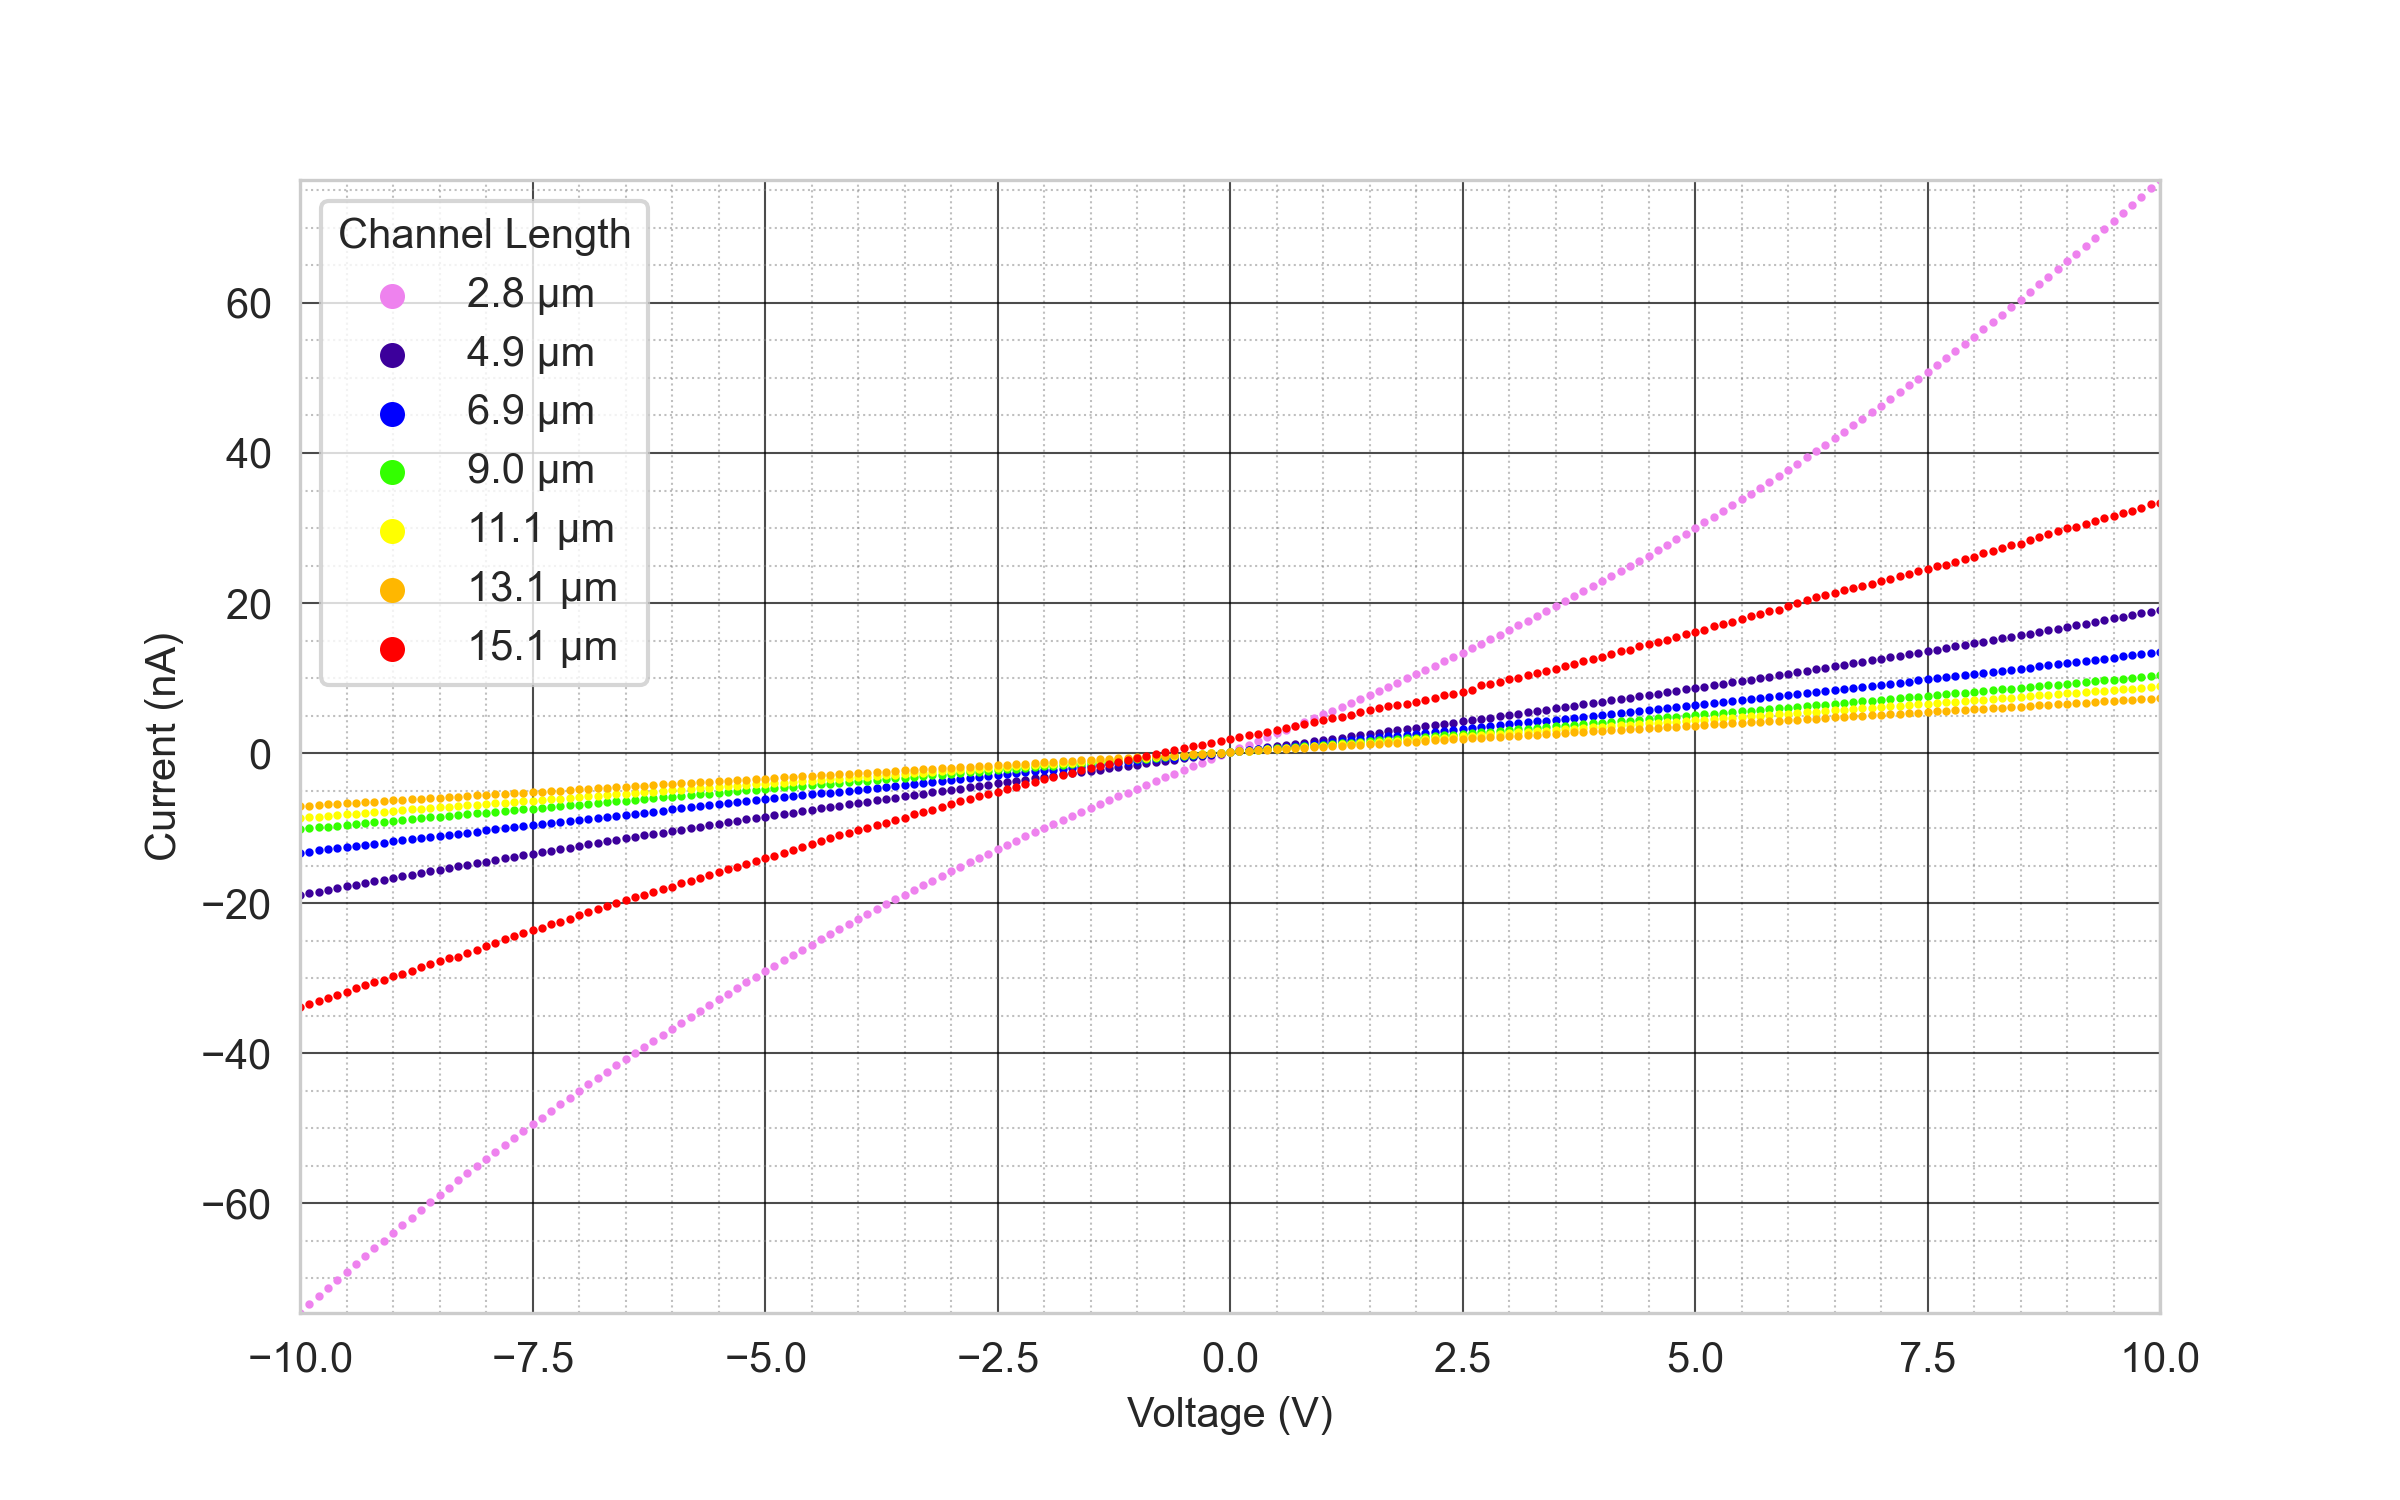
\includegraphics[width=0.97\textwidth]{Chapter3/Figs/Raster/Sample D 2019/IV/10V IV characteristics at 300 C.png}
    \caption{A linear plot of the measured current against applied voltage for all channel lengths at 300\si{\degreeCelsius} (sample D).}
    \label{appfig:D_current_voltage_300_10V}
\end{figure}

\subsection{Sample D: 50 \si{\volt} range}
\begin{figure}[h]
    \centering
    \includegraphics[width=0.97\textwidth]{Chapter3/Figs/Raster/Sample D 2019/IV/50v IV characteristics at 21 C.png}
    \caption{A linear plot of the measured current against applied voltage for all channel lengths at 21\si{\degreeCelsius} (sample D).}
    \label{appfig:D_current_voltage_21_50v}
\end{figure}
\begin{figure}[h]
    \centering
    \includegraphics[width=0.97\textwidth]{Chapter3/Figs/Raster/Sample D 2019/IV/50v IV characteristics at 50 C.png}
    \caption{A linear plot of the measured current against applied voltage for all channel lengths at 50\si{\degreeCelsius} (sample D).}
    \label{appfig:D_current_voltage_50_50v}
\end{figure}
\begin{figure}[h]
    \centering
    \includegraphics[width=0.97\textwidth]{Chapter3/Figs/Raster/Sample D 2019/IV/50v IV characteristics at 100 C.png}
    \caption{A linear plot of the measured current against applied voltage for all channel lengths at 100\si{\degreeCelsius} (sample D).}
    \label{appfig:D_current_voltage_100_50v}
\end{figure}
\begin{figure}[h]
    \centering
    \includegraphics[width=0.97\textwidth]{Chapter3/Figs/Raster/Sample D 2019/IV/50v IV characteristics at 150 C.png}
    \caption{A linear plot of the measured current against applied voltage for all channel lengths at 150\si{\degreeCelsius} (sample D).}
    \label{appfig:D_current_voltage_150_50v}
\end{figure}
\begin{figure}[h]
    \centering
    \includegraphics[width=0.97\textwidth]{Chapter3/Figs/Raster/Sample D 2019/IV/50v IV characteristics at 200 C.png}
    \caption{A linear plot of the measured current against applied voltage for all channel lengths at 200\si{\degreeCelsius} (sample D).}
    \label{appfig:D_current_voltage_200_50v}
\end{figure}
\begin{figure}[h]
    \centering
    \includegraphics[width=0.97\textwidth]{Chapter3/Figs/Raster/Sample D 2019/IV/50v IV characteristics at 250 C.png}
    \caption{A linear plot of the measured current against applied voltage for all channel lengths at 250\si{\degreeCelsius} (sample D).}
    \label{appfig:D_current_voltage_250_50v}
\end{figure}
\begin{figure}[h]
    \centering
    \includegraphics[width=0.97\textwidth]{Chapter3/Figs/Raster/Sample D 2019/IV/50v IV characteristics at 300 C.png}
    \caption{A linear plot of the measured current against applied voltage for all channel lengths at 300\si{\degreeCelsius} (sample D).}
    \label{appfig:D_current_voltage_300_50v}
\end{figure}
\label{app:I_V_sample_D_50V}

\subsection{Pre-Annealing Electrical Characterisation}
\subsubsection{I-V Plots}
\begin{figure}[H]
    \centering
    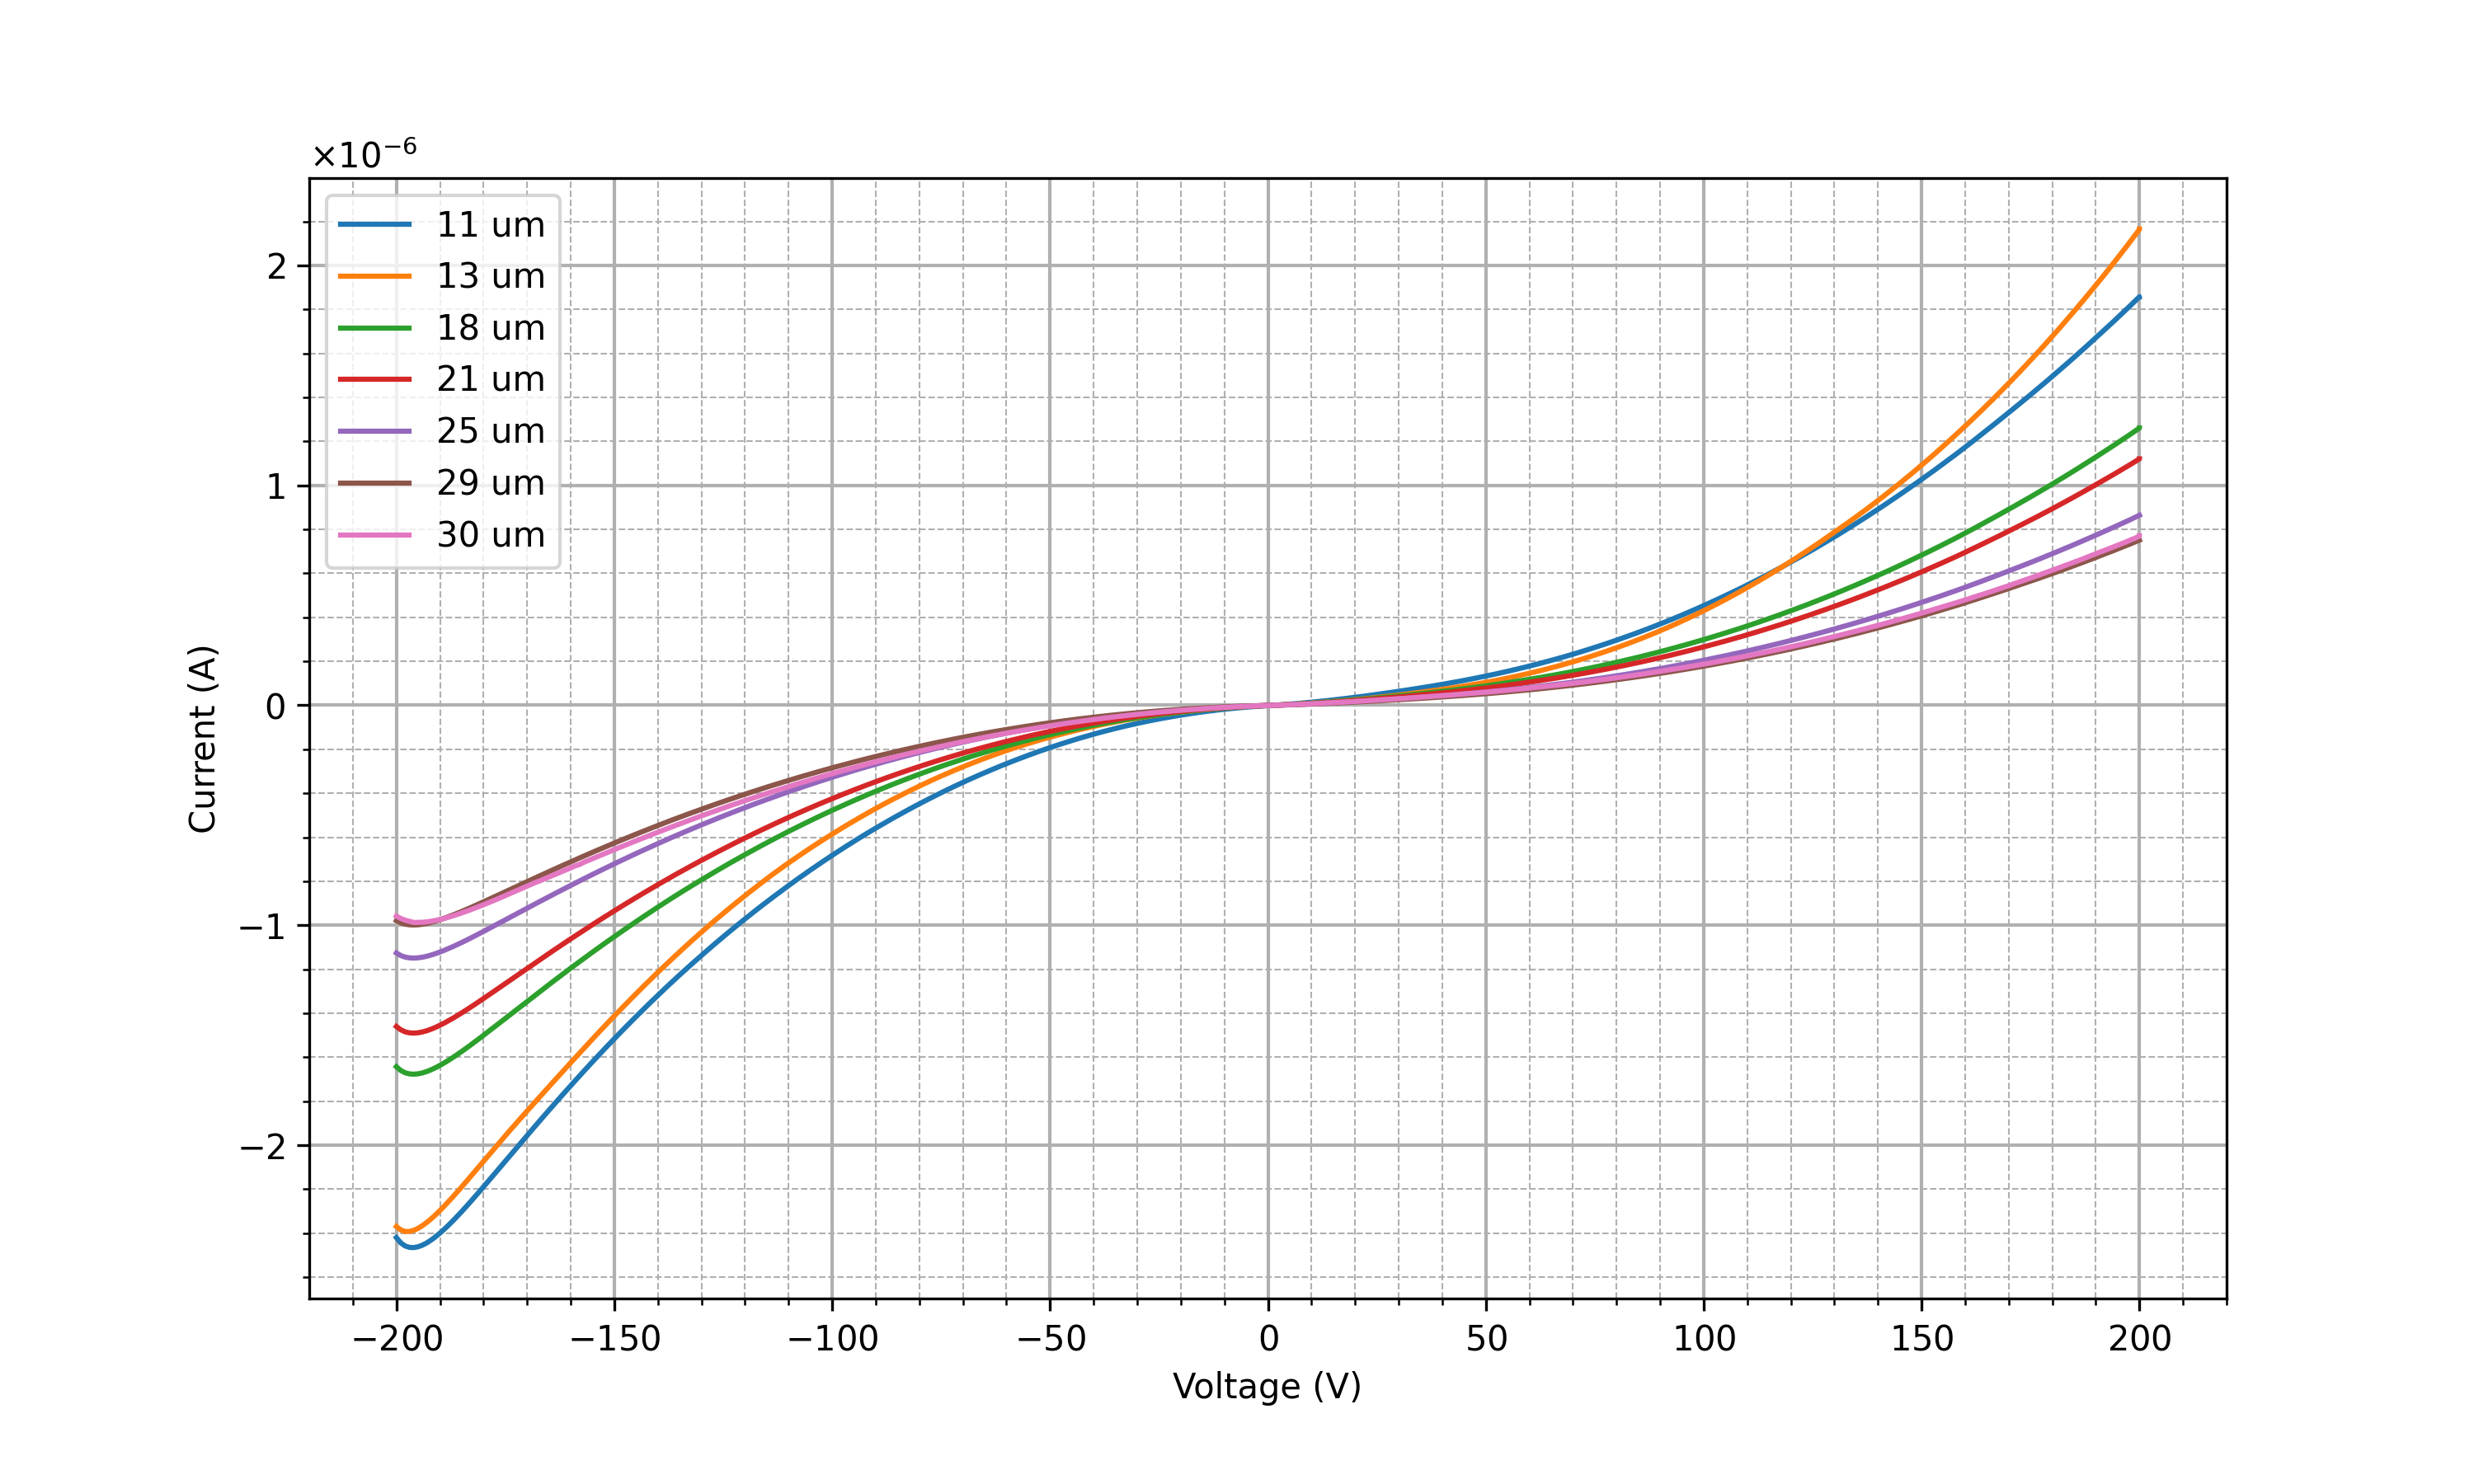
\includegraphics[width=\textwidth]{Chapter3/Figs/Raster/Sample F 2022/Pre-anneal data/lin_scale.png}
    \caption{Pre-annealing I-V data for the full bias range ($\pm200$ \si{\volt}), across the selected channels.}
    \label{fig:pre-anneal-iv-lin-200}
\end{figure}
\begin{figure}[H]
    \centering
    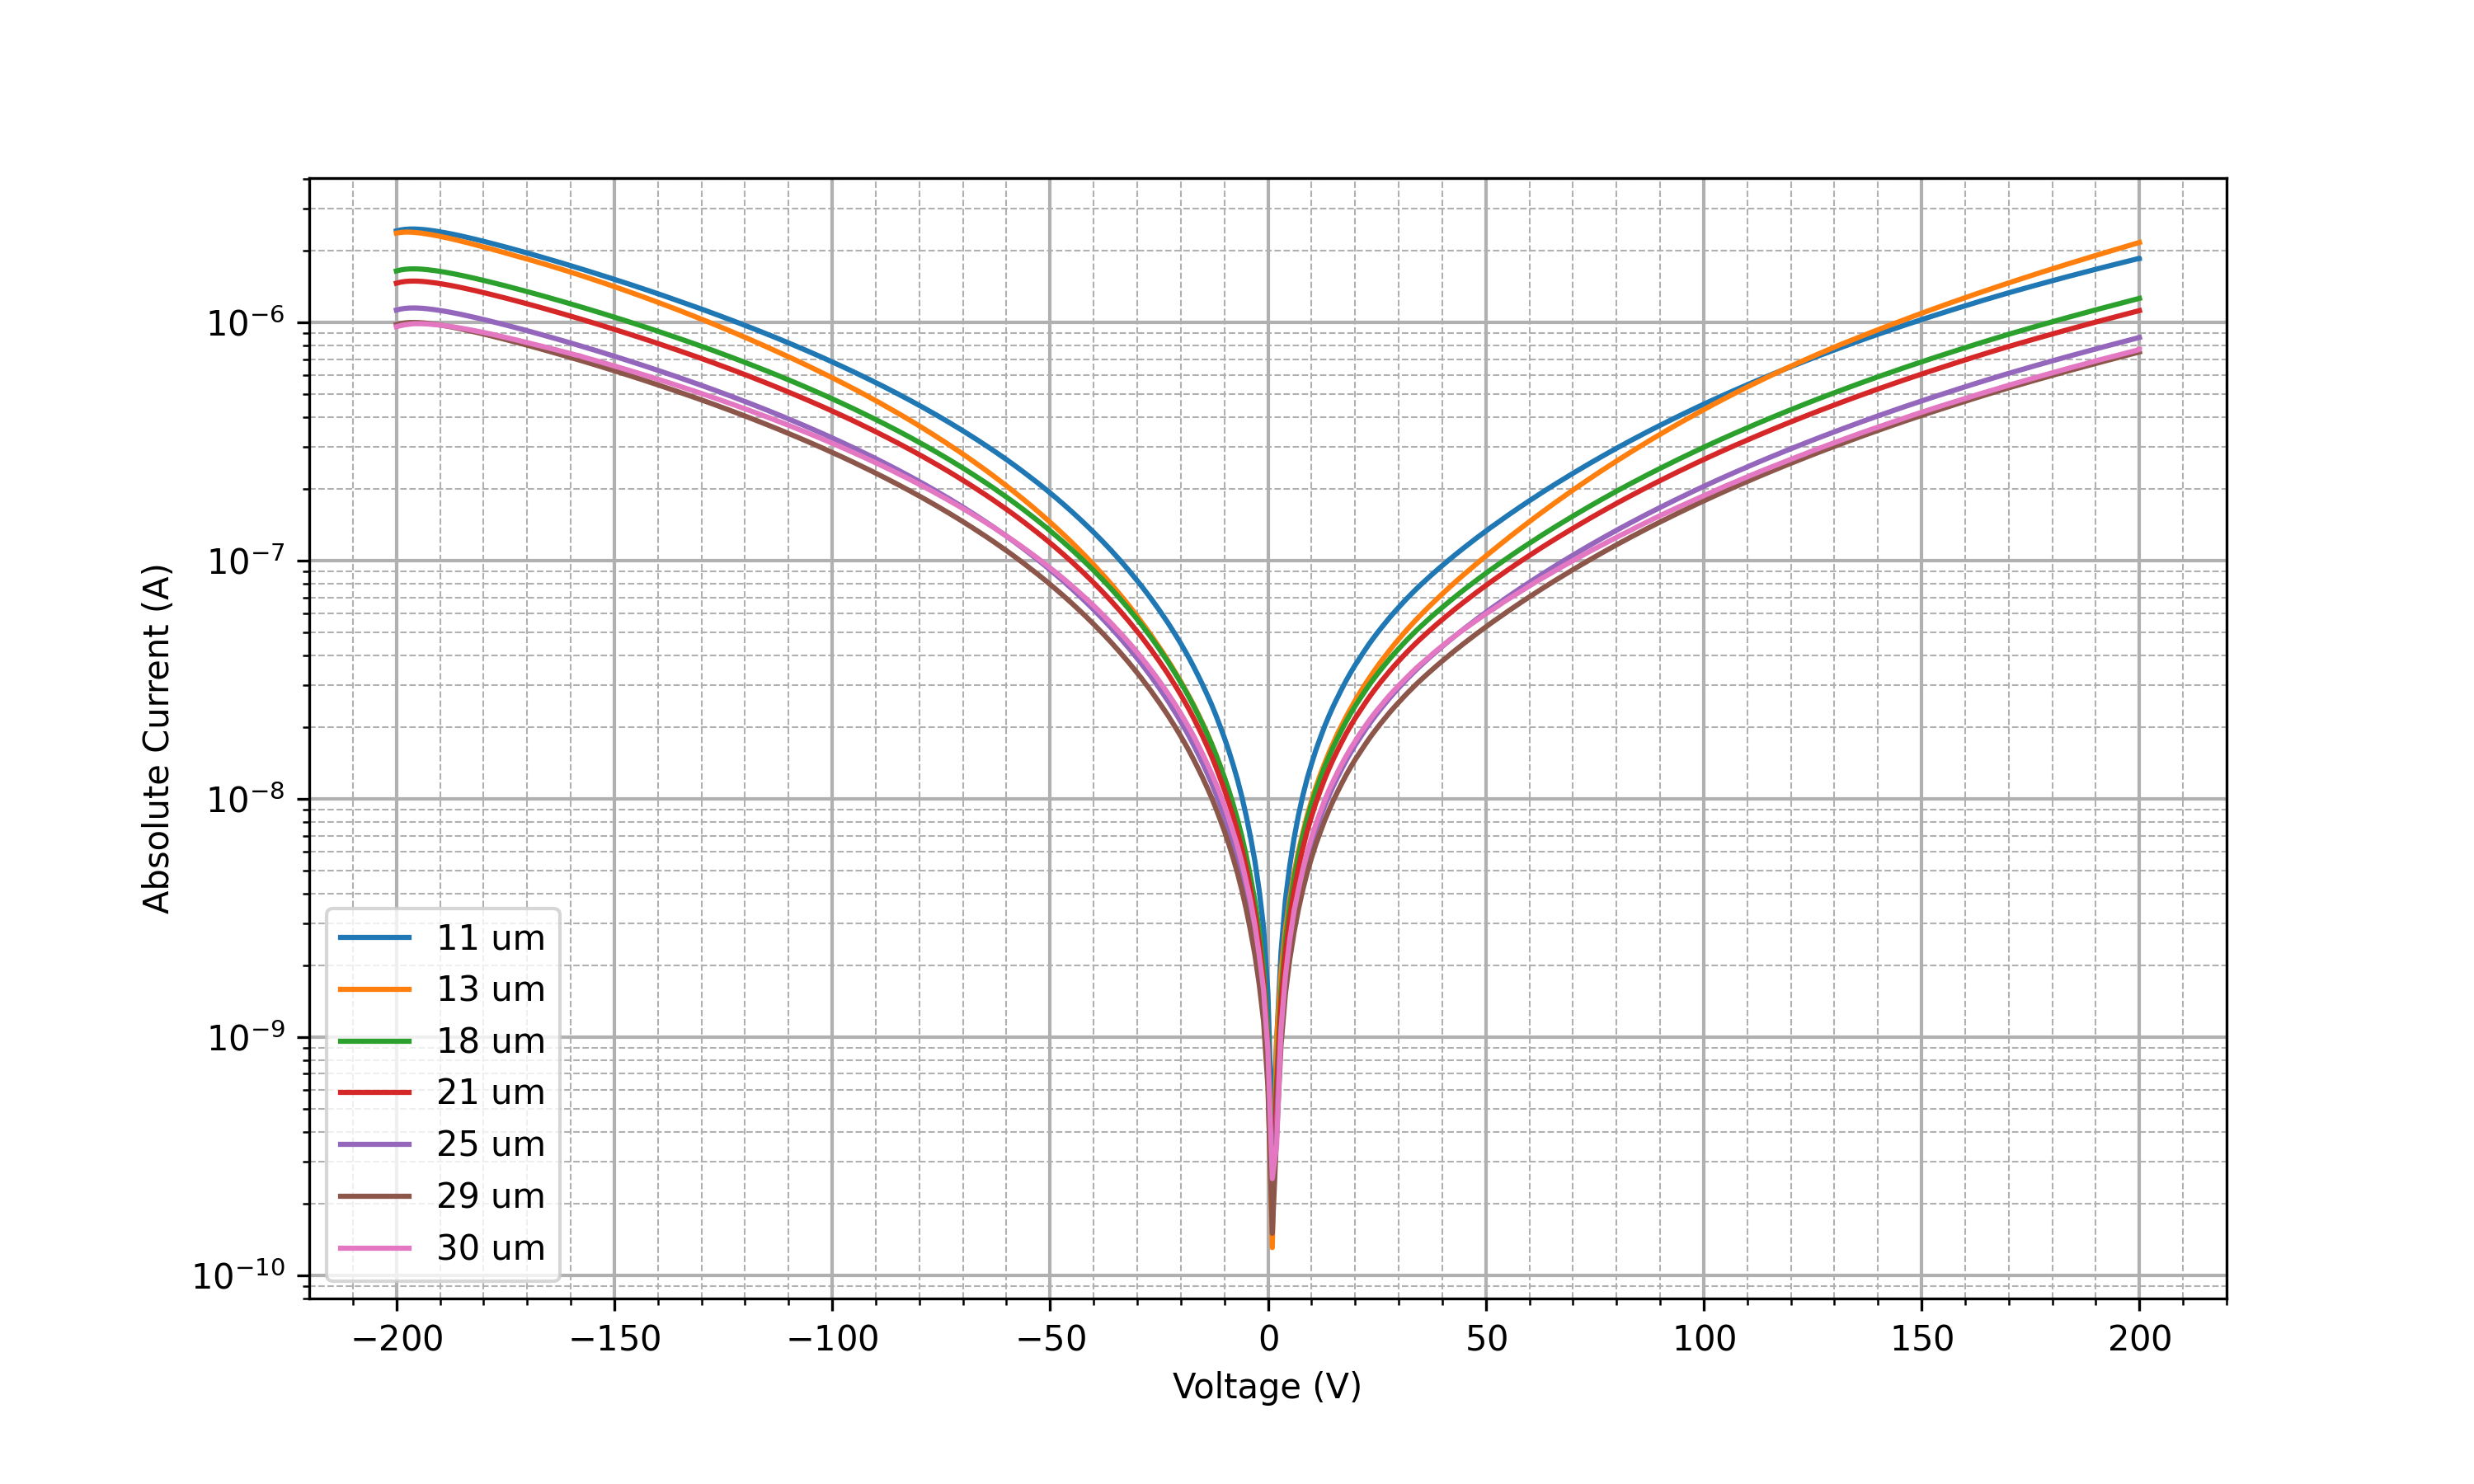
\includegraphics[width=\textwidth]{Chapter3/Figs/Raster/Sample F 2022/Pre-anneal data/log_scale.png}
    \caption{Pre-annealing I-V data for the full bias range ($\pm200$ \si{\volt}), logarithmic current scale.}
    \label{fig:pre-anneal-iv-log-200}
\end{figure}

\subsubsection{CTLM Plots}
As discussed earlier, for a circular TLM comparison, specific values of the current must be chosen for $I_{0}$, this value can hence be selected to reflect the low voltage region of the current-voltage behaviour, or the higher voltage region, resulting in the following resistance-spacing graphs, from high currents to low currents:

\begin{figure}[H]
    \centering
    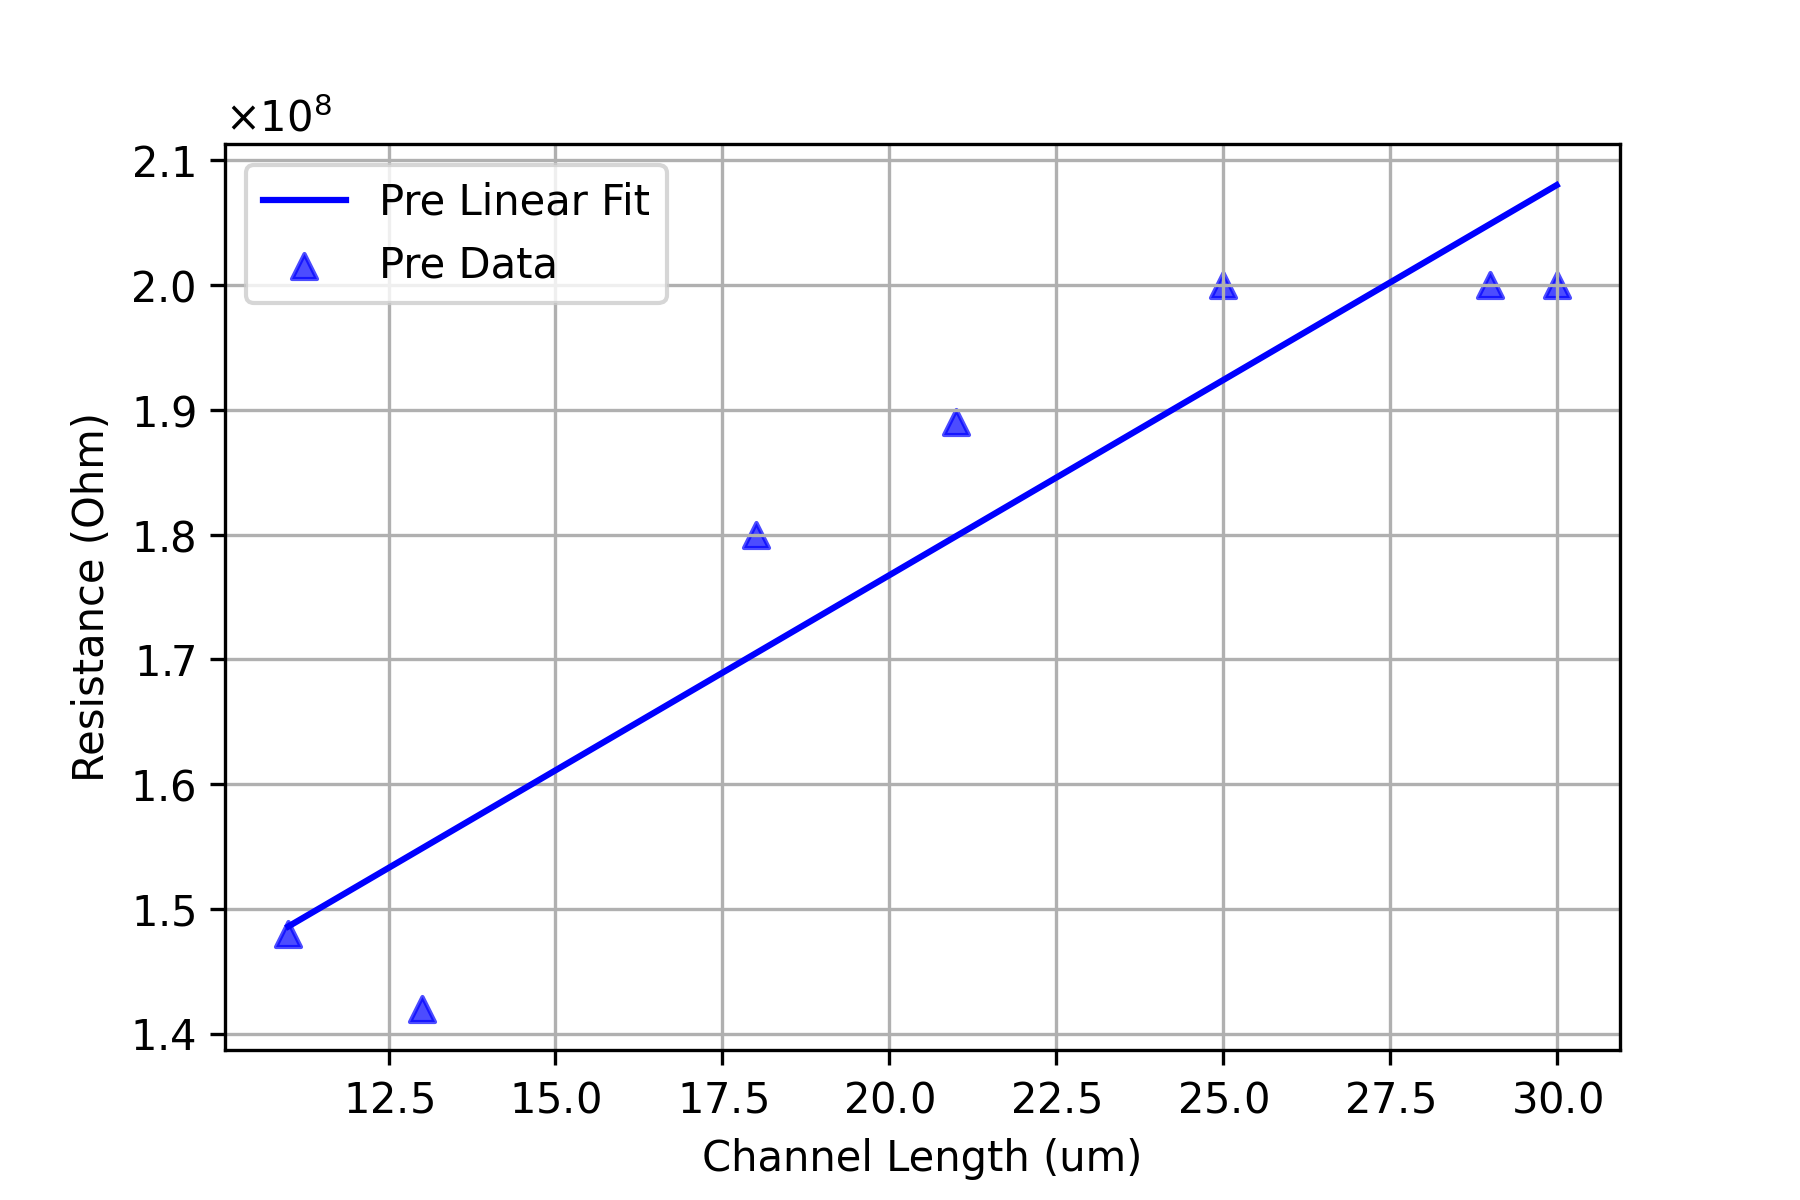
\includegraphics[width=\textwidth]{Chapter3/Figs/Raster/Sample F 2022/Pre-anneal data/1e-06A.png}
    \caption{Pre-annealing d-R data for $I_{0}=1\times10^{-6}$ \si{\ampere}, across the selected channels. Linear fit: $y = 3.126\times10^{6}x + 1.142\times10^{8}$, $R^{2}=0.870$.}
    \label{fig:pre-anneal-dr-1e-6}
\end{figure}
\begin{figure}[H]
    \centering
    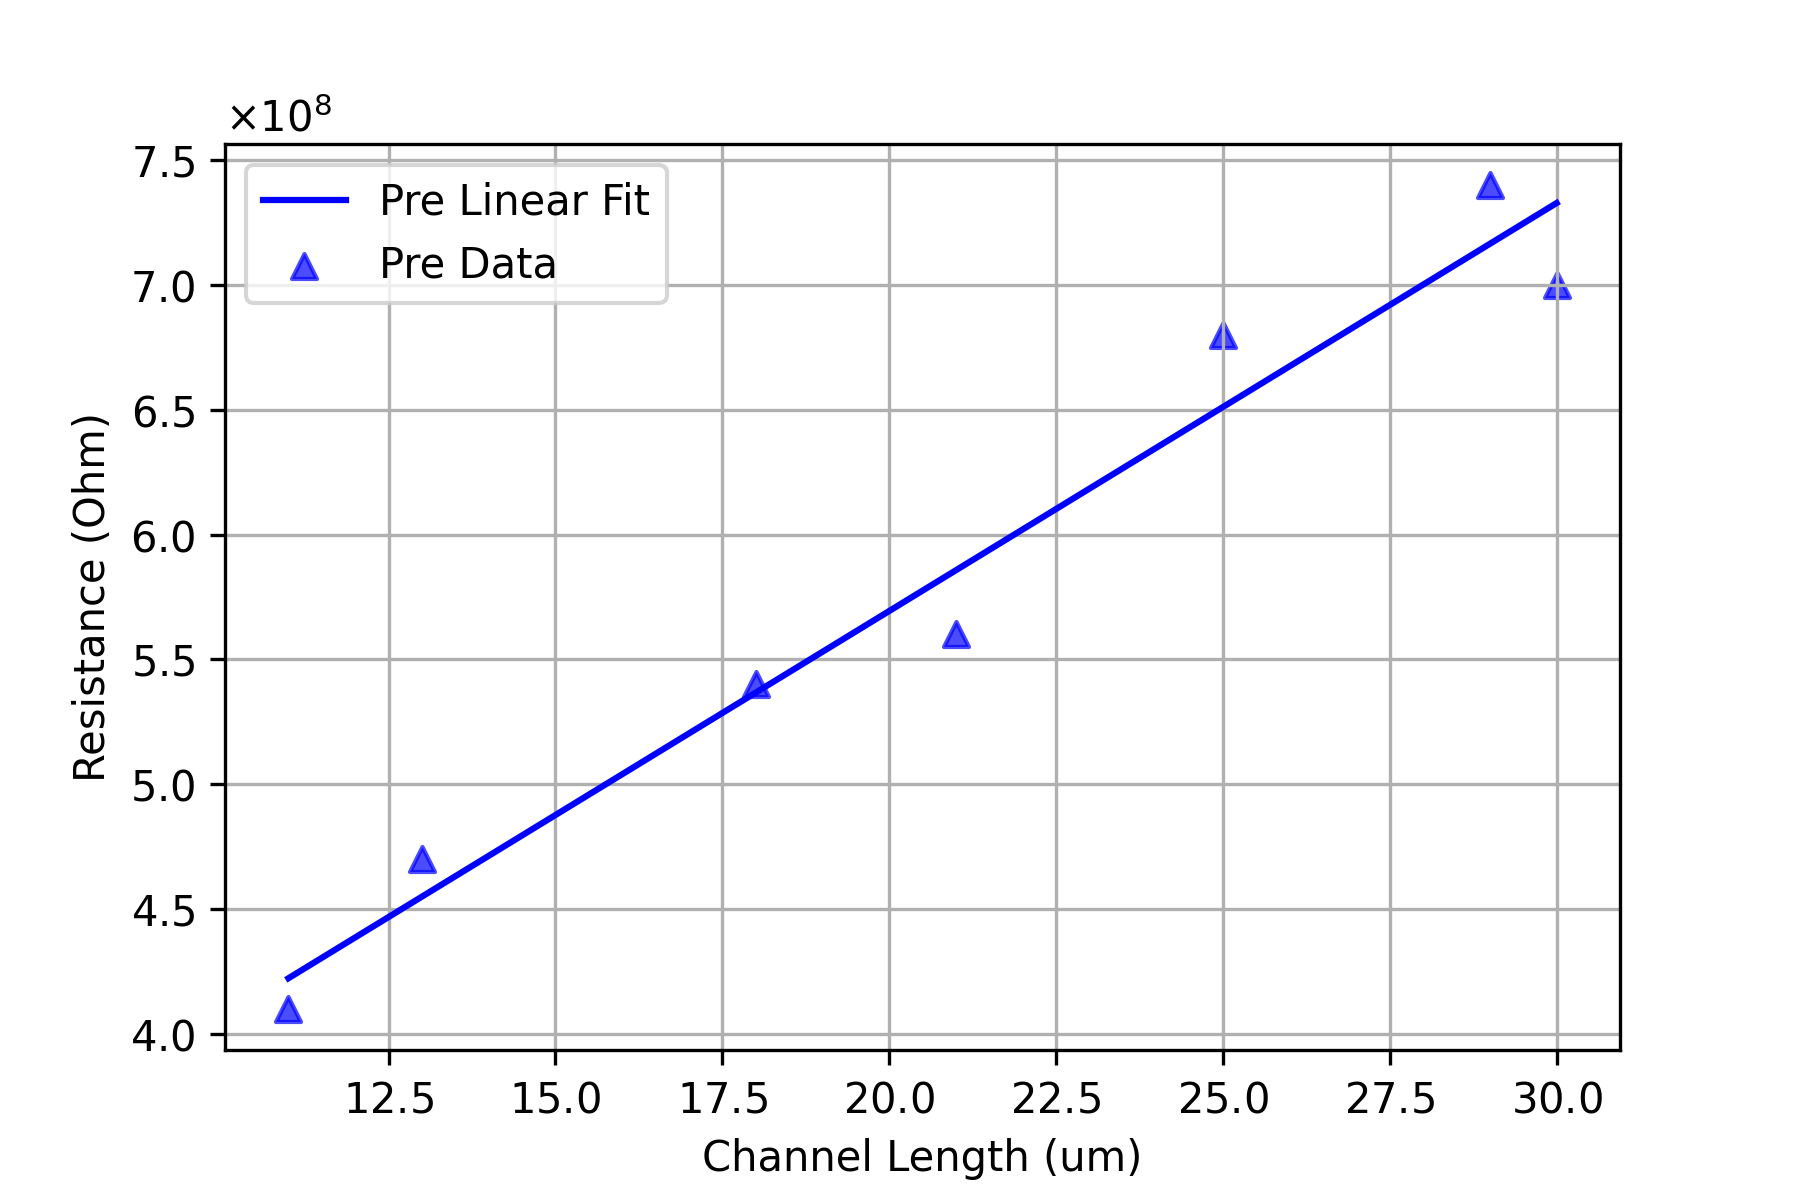
\includegraphics[width=\textwidth]{Chapter3/Figs/Raster/Sample F 2022/Pre-anneal data/1e-07A.png}
    \caption{Pre-annealing d-R data for $I_{0}=1\times10^{-7}$ \si{\ampere}, across the selected channels. Linear fit: $y = 1.635\times10^{7}x + 2.424\times10^{8}$, $R^{2}=0.962$.}
    \label{fig:pre-anneal-dr-1e-7}
\end{figure}
\begin{figure}[H]
    \centering
    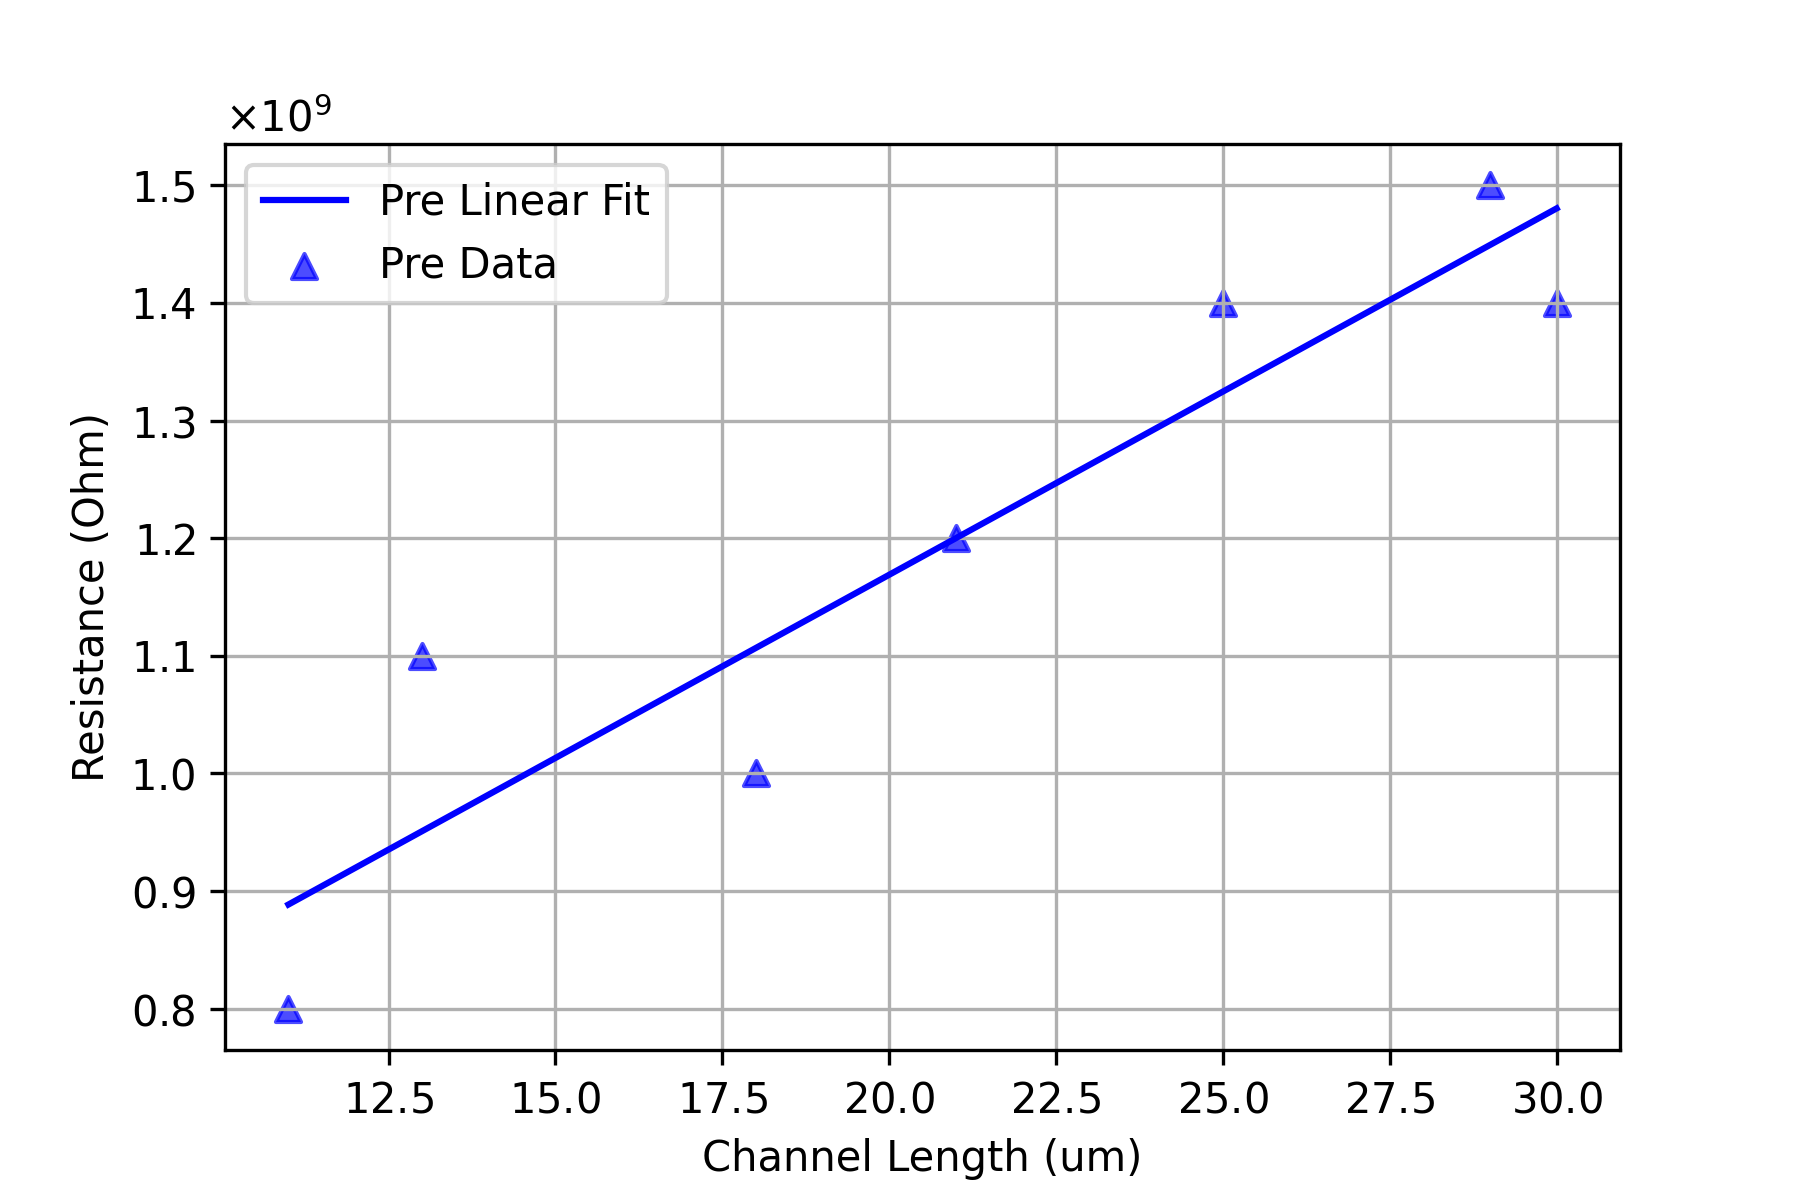
\includegraphics[width=\textwidth]{Chapter3/Figs/Raster/Sample F 2022/Pre-anneal data/1e-08A.png}
    \caption{Pre-annealing d-R data for $I_{0}=1\times10^{-8}$ \si{\ampere}, across the selected channels. Linear fit: $y = 3.114\times10^{7}x + 5.461\times10^{8}$, $R^{2}=0.852$.}
    \label{fig:pre-anneal-dr-1e-8}
\end{figure}
\begin{figure}[H]
    \centering
    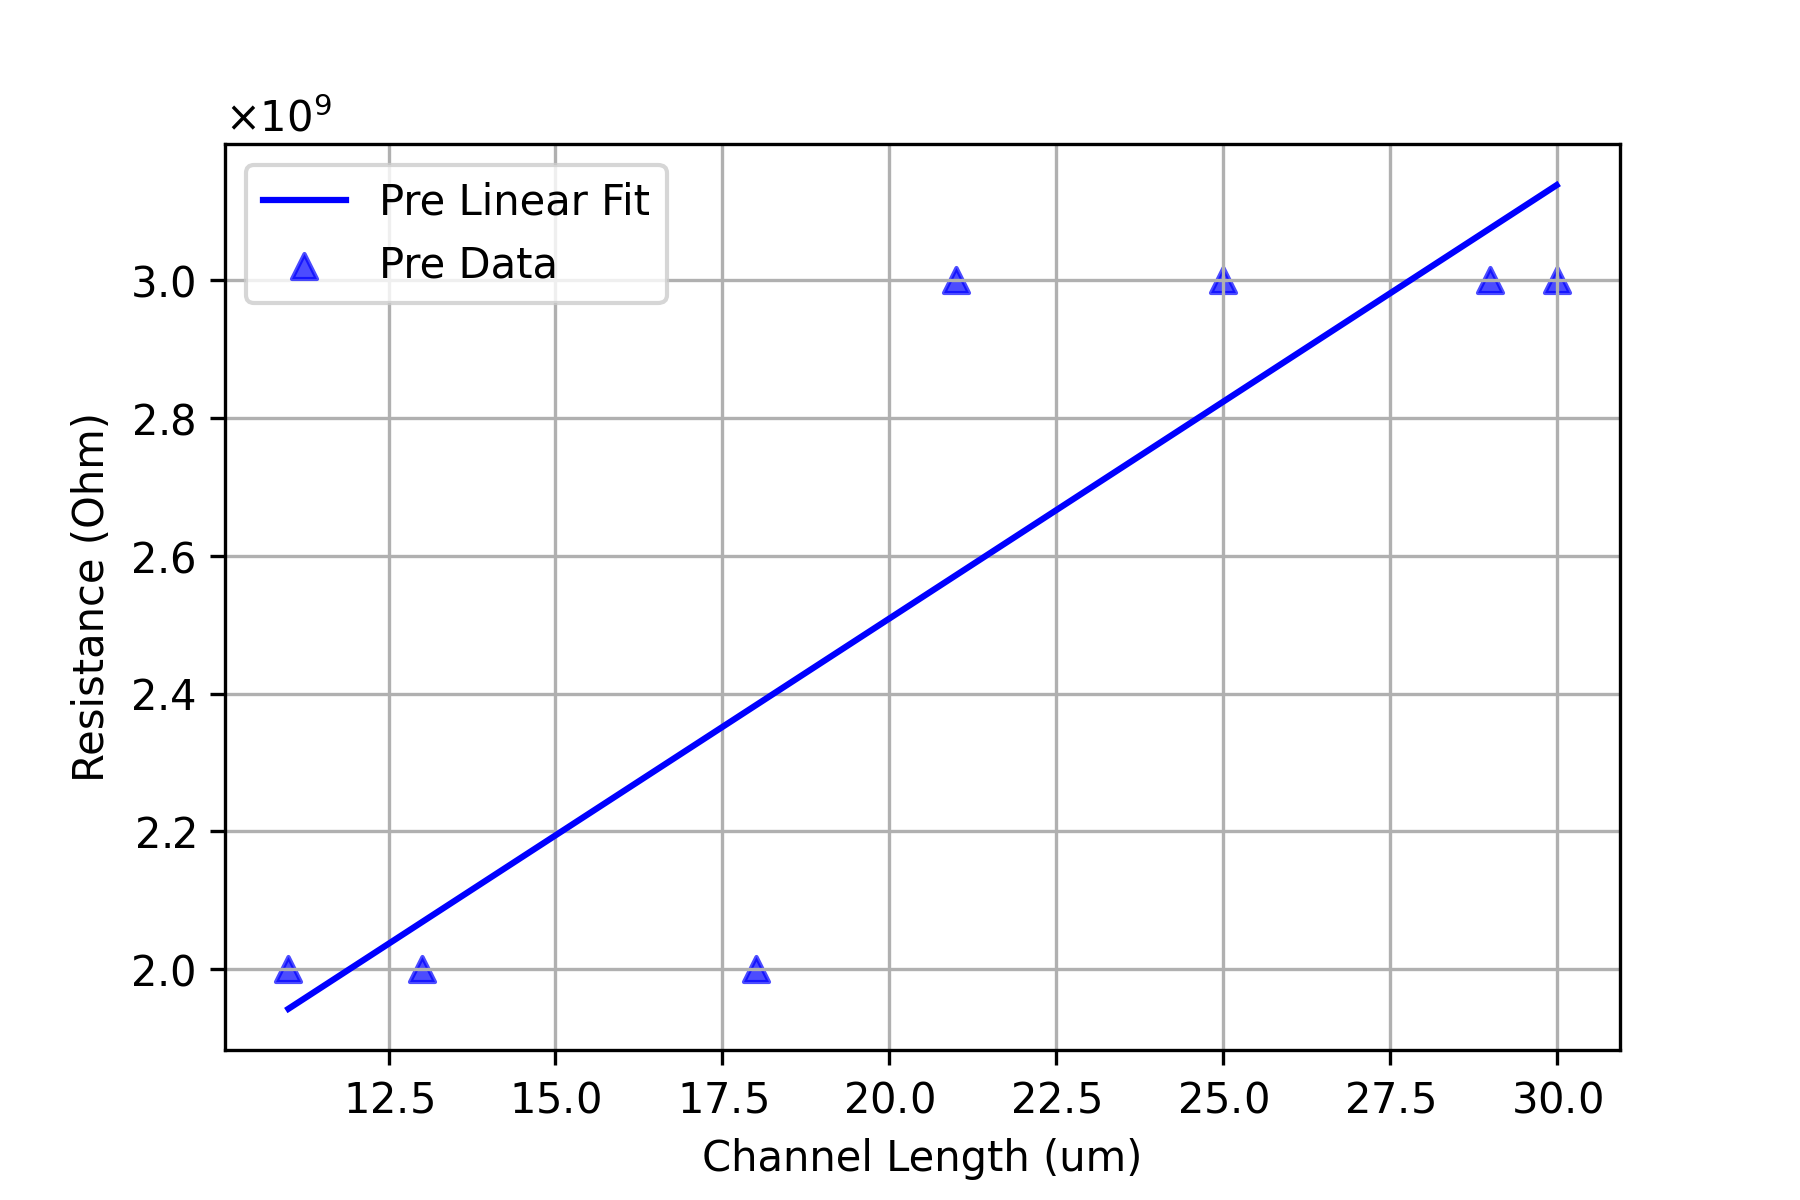
\includegraphics[width=\textwidth]{Chapter3/Figs/Raster/Sample F 2022/Pre-anneal data/1e-09A.png}
    \caption{Pre-annealing d-R data for $I_{0}=1\times10^{-9}$ \si{\ampere}, across the selected channels. Linear fit: $y = 6.287\times10^{7}x + 1.251\times10^{9}$, $R^{2}=0.770$.}
    \label{fig:pre-anneal-dr-1e-9}
\end{figure}
\begin{comment}
\begin{table}[H]
\centering
\caption{Linear fit parameters for Pre-annealing d-R data}
\label{tab:linear-fits}
\begin{tabular}{|c|c|c|c|}
\hline
\textbf{$I_0$ (\si{\ampere})} & \textbf{Slope ($\Omega/\mu$m)} & \textbf{Intercept ($\Omega$)}  & \textbf{$R^{2}$} \\ \hline
$1\times10^{-6}$ & $3.126\times10^{6}$ & $1.142\times10^{8}$ & $0.870$\\ \hline
$1\times10^{-7}$ & $1.635\times10^{7}$ & $2.424\times10^{8}$ & $0.962$\\ \hline
$1\times10^{-8}$ & $3.114\times10^{7}$ & $5.461\times10^{8}$ & $0.852$\\ \hline
$1\times10^{-9}$ & $6.287\times10^{7}$ & $1.251\times10^{9}$ & $0.770$\\ \hline
\end{tabular}
\end{table}
\end{comment}
\subsection{Post-Annealing Electrical Characterisation}
\subsubsection{I-V Plots}
\begin{figure}[H]
    \centering
    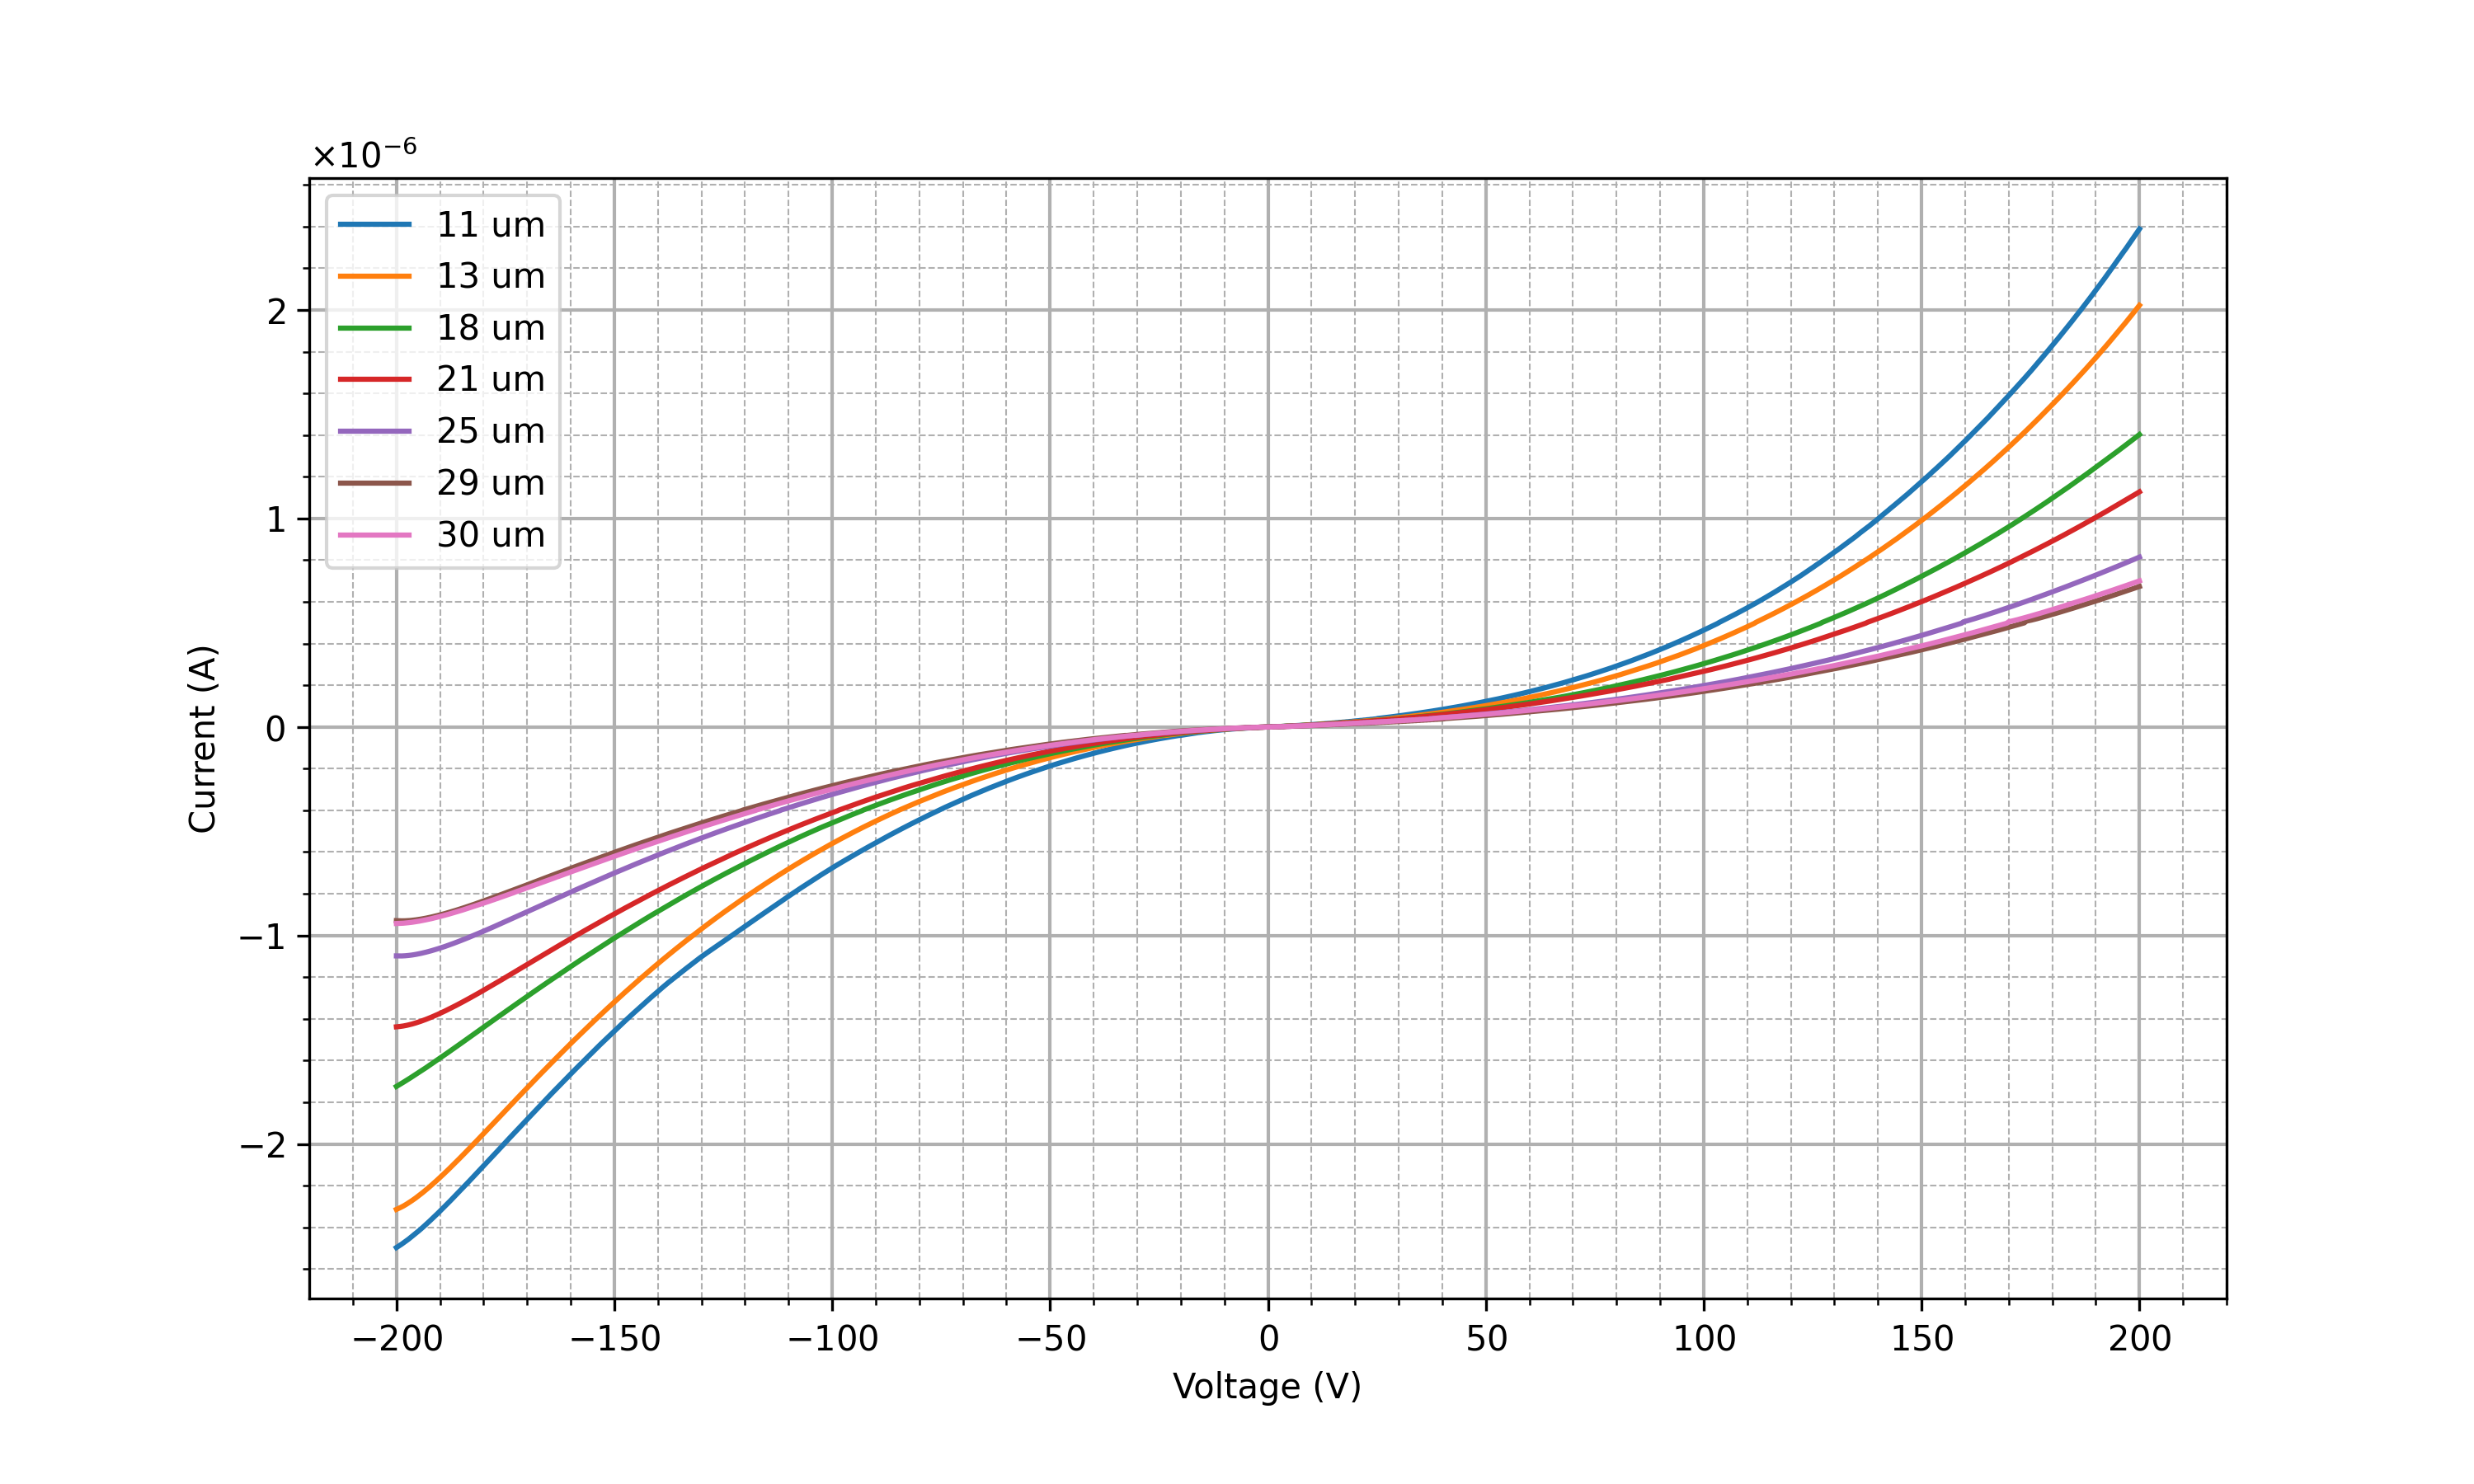
\includegraphics[width=\textwidth]{Chapter3/Figs/Raster/Sample F 2022/Post-anneal/lin_scale.png}
    \caption{Post-annealing I-V data for the full bias range ($\pm200$ \si{\volt}), across the selected channels.}
    \label{fig:post-anneal-iv-lin-200}
\end{figure}
\begin{figure}[H]
    \centering
    \includegraphics[width=\textwidth]{Chapter3/Figs/Raster/Sample F 2022/Post-anneal/log_scale.png}
    \caption{Post-annealing I-V data for the full bias range ($\pm200$ \si{\volt}), logarithmic current scale.}
    \label{fig:post-anneal-iv-log-200}
\end{figure}

\subsubsection{CTLM Plots}

\begin{figure}[h]
    \centering
    \includegraphics[width=\textwidth]{Chapter3/Figs/Raster/Sample F 2022/Post-anneal/1e-06A.png}
    \caption{Post-annealing d-R data for $I_{0}=1\times10^{-6}$ \si{\ampere}, across the selected channels. Linear fit: $y = 3.229\times10^{6}x + 1.112\times10^{8}$, $R^{2}=0.913$.}
    \label{fig:post-anneal-dr-1e-6}
\end{figure}
\begin{figure}[H]
    \centering
    \includegraphics[width=\textwidth]{Chapter3/Figs/Raster/Sample F 2022/Post-anneal/1e-07A.png}
    \caption{Post-annealing d-R data for $I_{0}=1\times10^{-7}$ \si{\ampere}, across the selected channels. Linear fit: $y = 1.431\times10^{7}x + 2.915\times10^{8}$, $R^{2}=0.955$.}
    \label{fig:post-anneal-dr-1e-7}
\end{figure}
\begin{figure}[H]
    \centering
    \includegraphics[width=\textwidth]{Chapter3/Figs/Raster/Sample F 2022/Post-anneal/1e-08A.png}
    \caption{Post-annealing d-R data for $I_{0}=1\times10^{-8}$ \si{\ampere}, across the selected channels. Linear fit: $y = 2.000\times10^{7}x + 7.057\times10^{8}$, $R^{2}=0.899$.}
    \label{fig:post-anneal-dr-1e-8}
\end{figure}
\begin{figure}[H]
    \centering
    \includegraphics[width=\textwidth]{Chapter3/Figs/Raster/Sample F 2022/Post-anneal/1e-09A.png}
    \caption{Post-annealing d-R data for $I_{0}=1\times10^{-9}$ \si{\ampere}, across the selected channels. Linear fit: $y = 4.671\times10^{7}x + 5.049\times10^{8}$, $R^{2}=0.295$.}
    \label{fig:post-anneal-dr-1e-9}
\end{figure}

\begin{table}[h]
\centering
\caption{Linear fit parameters for Post-annealing d-R data}
\label{tab:post-linear-fits}
\begin{tabular}{|c|c|c|c|}
\hline
\textbf{$I_0$ (\si{\ampere})} & \textbf{Slope ($\Omega/\mu$m)} & \textbf{Intercept ($\Omega$)}  & \textbf{$R^{2}$} \\ \hline
$1\times10^{-6}$ & $3.229\times10^{6}$ & $1.112\times10^{8}$ & $0.913$ \\ \hline
$1\times10^{-7}$ & $1.431\times10^{7}$ & $2.915\times10^{8}$ & $0.955$ \\ \hline
$1\times10^{-8}$ & $2.000\times10^{7}$ & $7.057\times10^{8}$ & $0.899$ \\ \hline
$1\times10^{-9}$ & $4.671\times10^{7}$ & $5.049\times10^{8}$ & $0.295$ \\ \hline
\end{tabular}
\end{table}